\documentclass[12pt, a4paper]{article}
\usepackage[utf8]{inputenc}

\usepackage{hyperref}
\usepackage{float} % To use 'H' for figures
\usepackage{graphicx} % to display images
\usepackage[dvipsnames]{xcolor} % to use colours
\usepackage{amssymb} % For 'mathbb'

\usepackage[normalem]{ulem} % underlying that breaks at line end

\usepackage{amsmath} % for advanced math formatting
\DeclareMathOperator*{\argmax}{arg\,max} % declare \argmax
\usepackage{amssymb} % for advanced math formatting

\usepackage{titlesec} % Title/Section Styling

\let\stdsection\section
\renewcommand\section{\newpage\stdsection} % Start each section from new page

\titleformat{\section} % uline sections
  {\normalfont\Large\bfseries}{\thesection}{1em}{}[{\titlerule[0.8pt]}]

\usepackage{tcolorbox} % for creating boxes

\setcounter{secnumdepth}{5}
\setcounter{tocdepth}{5}
\makeatletter
\newcommand\subsubsubsection{\@startsection{paragraph}{4}{\z@}{-2.5ex\@plus -1ex \@minus -.25ex}{1.25ex \@plus .25ex}{\normalfont\normalsize\bfseries}}
\newcommand\subsubsubsubsection{\@startsection{subparagraph}{5}{\z@}{-2.5ex\@plus -1ex \@minus -.25ex}{1.25ex \@plus .25ex}{\normalfont\normalsize\bfseries}}
\makeatother

\setlength{\parindent}{0em}
\setlength{\parskip}{1em}

\title{Reinforcement Learning NOTES}
\author{Kristian Bonnici}


\begin{document}



\maketitle
\tableofcontents

\newpage
\subsection{Summary of Notation}\label{summary-of-notation}

\(\dot{=}\) is used for \textbf{``is defined as''}

\(S =\) set of \textbf{nonterminal states} * \(s, s' \rightarrow\) some
states

\(S^+ =\) set of \textbf{all states}, including the terminal state

\(A =\) set of \textbf{actions}

\(R =\) set of \textbf{rewards}

We'll assume that each of these sets will have a \emph{finite number of
elements}.

\(T \rightarrow\) transition function

\(V, V_t\) \(\rightarrow\) array \textbf{estimates} of
\(v_\pi(s)\) or \(v_*(s)\)

\(v_*(s) \rightarrow\) value of state s under the optimal policy
\begin{itemize}
  \item $= \max_\pi v_\pi(s)$
\end{itemize}

\(Q, Q_t\) \(\rightarrow\) array \textbf{estimates} of
\(q_\pi(s,a)\) or \(q_*(s,a)\)



\textcolor{blue}{\textbf{Return $G$:}} is the total of rewards

\begin{itemize}
  \item \textbf{$G$ for Episodic Tasks:} The return at time step $t$ is the \uline{sum of rewards until termination}.
  $$
  G_t \dot{=} R_{t+1} + R_{t+2} + R_{t+3} + ... + R_T
  $$
  \item \textbf{$G$ for Continuing Tasks:} \uline{sum of discounted future rewards} (made to be always finite).
  \begin{align*}
    G_t &\dot{=} R_{t+1} + \gamma R_{t+2} + \gamma^2 R_{t+3} + ... + R_{t+k} + ... \\
    &\dot{=} \sum_{k=0}^{\infty} \gamma^k R_{t+k+1}
  \end{align*}
  \begin{itemize}
    \item \textbf{(recursively):}
    $$
    G_t \dot{=} R_{t+1} + \gamma G_{t+1}
    $$
  \end{itemize}
  \item Where:
  \begin{itemize}
    \item
      \(\gamma =\) is a parameter, \(0 \leq \gamma \leq 1\), called the
      \textbf{discount rate}.
      \begin{itemize}
        \item If $\gamma = 1$, undiscounted.
      \end{itemize}
  \end{itemize}
\end{itemize}





\textcolor{blue}{\textbf{Value functions:}}

\begin{itemize}
  \item The current time-step's \uline{state/action values} can be written \textbf{recursively} in terms of \textbf{future state/action values} with \textcolor{blue}{\textbf{Bellman equations}}.
\end{itemize}

\begin{itemize}
  \item \textcolor{blue}{\textbf{State-Value functions:}} \uline{expected return $G$ from a given state $s$}, following policy $\pi$.
  $$
  v_\pi (s) = \mathbb{E}_\pi[G_t|S_t=s]
  $$
  \begin{itemize}
  \item \textbf{(recursively):}
    $$
    v_\pi(s) = \mathbb{E}_\pi[\underbrace{R_{t+1}}_\text{immediate reward} + \underbrace{\gamma G_{t+1}}_\text{discounted return at time $t + 1$}|S_t=s]
    $$
  \item \textbf{(State-Value Bellman equation):}
    \begin{align*}
    \textcolor[HTML]{8F5760}{v_\pi(s)} &\dot{=} \textcolor[HTML]{8F5760}{\mathbb{E}_\pi[G_t|S_t=s]} \\
    &= \sum_a \pi(a|s) \sum_{s'} \sum_{r} p(s',r|s,a) [r + \gamma \textcolor[HTML]{8F5760}{\mathbb{E}_\pi[G_{t+1}|S_{t+1}=s']}] \\
    &= \underbrace{\sum_a \pi(a|s)}_\text{sum over possible action choices } \underbrace{\sum_{s'} \sum_{r} p(s',r|s,a)}_\text{ sum over possible rewards and next states} [r + \gamma \textcolor[HTML]{8F5760}{v_\pi(s')}]
    \end{align*}
    \begin{itemize}
      \item The result is a \uline{weighted sum} of terms consisting of immediate reward plus expected future returns from the next state $s'$.
    \end{itemize}

    \item \textbf{(State-Value Bellman Optimality equation):}
      $$
      v_*(s) = \max_a \sum_{s'} \sum_{r} p(s',r|s,a) [r + \gamma v_*(s')]
      $$

  \item The magic of value functions is that we can use them as a stand-in for the average of an infinite number of possible futures.
  \end{itemize}
\end{itemize}



\begin{itemize}
  \item
  \textcolor{blue}{\textbf{Action-Value functions:}} \uline{expected return $G$ if the agent selects action $a$ in state $s$} and then follows policy $\pi$ thereafter.
    $$
    q_\pi(s,a) = \mathbb{E}_\pi[G_t | S_t=s, A_t = a]
    $$
    \begin{itemize}
      \item \textbf{(Action-Value Bellman equation):}
        \begin{align*}
        \textcolor[HTML]{8F5760}{q_\pi(s, a)} &\dot{=} \textcolor[HTML]{8F5760}{\mathbb{E}_\pi[G_t | S_t=s, A_t = a]} \\
        &= \sum_{s'} \sum_{r} p(s',r|s,a) [r + \gamma \sum_{a'} \pi(a'|s') \textcolor[HTML]{8F5760}{\mathbb{E}_\pi[G_{t+1} | S_{t+1}=s', A_{t+1} = a']}] \\
        &= \sum_{s'} \sum_{r} p(s',r|s,a) [r + \gamma \sum_{a'} \pi(a'|s') \textcolor[HTML]{8F5760}{q_\pi(s', a')}]
        \end{align*}

        \item \textbf{(Action-Value Bellman Optimality equation):}
          $$
          q_*(s, a) = \sum_{s'} \sum_{r} p(s',r|s,a) [r + \gamma \max_{a'} q_*(s', a')]
          $$
    \end{itemize}
\end{itemize}





\textcolor{blue}{\textbf{Policy \(\pi\):}} mapping from state to action (decision-making rule)

\begin{itemize}
  \item \textbf{Deterministic policy notation:} $\pi(s)=a$
  \item \textbf{Stochastic policy notation:} $\pi(a|s)$
  \item \textbf{Optimal Policy \(\pi_*\)}
  \begin{align*}
    \text{for } q_*(s,a) \rightarrow \pi_*(s) &= \argmax_a q_*(s,a) \\
    \text{for } v_*(s) \rightarrow\ \pi_*(s) &= \argmax_a E_{s'}[r(s,a,s') + \gamma v_*(s')] \\
    &=  \argmax_a \sum_{s'} T(s,a,s') (r(s,a,s') + \gamma v_*(s'))
  \end{align*}

  \begin{itemize}
    \item With Bellman equation (compare to State/Action-Value Bellman Optimality equation):
    \begin{align*}
    \pi_*(s) &= \argmax_a \sum_{s'} \sum_{r} p(s',r|s,a) [r + \gamma v_*(s')] \\
    \pi_*(s) &= \argmax_a q_*(s,a)
    \end{align*}
  \end{itemize}
\end{itemize}

\begin{itemize}
\item
  \textbf{Value iteration:}, for estimating
  \(\pi \approx \pi_* \rightarrow \texttt{converges to } v_*(s)\). Only
  one iteration of iterative policy evaluation is performed between each
  step of policy improvement.

  \begin{itemize}
  \item
    Starting from \(V_0^*(s)=0\) for all (\(\forall\)) \(s\)
    \(\rightarrow\) iterate until convergence (usually change being
    smaller than some threshold we choose):

    \begin{itemize}
    \item
      \(V_{i+1}^*(s) = \max_a \sum_{s'} T(s,a,s') (r(s,a,s') + \gamma V_i^*(s'))\)
    \item
      \(\;\;\;\;\;\;\;\;\;\;\;\; = \max_a ImmediateReward + Discount*FutureRewards\)
    \end{itemize}
  \end{itemize}
\item
  \textbf{Policy iteration (iterative policy evaluation):}, for
  estimating \(\pi \approx \pi_*\).
\end{itemize}














\section{Introduction to Reinforcement Learning}\label{introduction-to-reinforcement-learning}

\textbf{Reinforcement learning} an area of machine learning concerned with how intelligent \textbf{agents} ought to take \textbf{actions} in an \textbf{environment} in order to maximize the notion of cumulative \textbf{reward}.

The \textbf{environment} is typically stated in the form of a Markov
decision process (MDP), because many reinforcement learning algorithms
for this context use dynamic programming techniques.

\textbf{Exploration \& Exploitation trade-off:} \textbf{Dilemma:}
choosing when to explore \& when to exploit?

\begin{itemize}
  \item \textbf{Exploration:} improve knowledge for long-term benefit.
  \item \textbf{Exploitation:} exploit knowledge for short-term benefit.
\end{itemize}

\textbf{Four main subelements of a reinforcement learning system:} a \textbf{policy}, a \textbf{reward signal}, a \textbf{value function}, and, optionally, a \textbf{model} of the environment.

\begin{itemize}
  \item \textbf{Policy} defines the learning agent's way of behaving at a given time.
  \item \textbf{Reward signal} indicates what is good in an immediate sense.
  \item \textbf{Value function} specifies what is good in the long run. Roughly speaking, the value of a state is the \emph{total amount of reward} an agent can expect to accumulate over the future, starting from that state.
  \item \textbf{Model} mimics the behaviour of the environment, or more generally, that allows inferences to be made about how the environment will behave.
  \begin{itemize}
    \item \textbf{Used for planning}, by which we mean any way of deciding on a course of action by considering possible future situations before they are actually experienced.
  \end{itemize}
\end{itemize}



\textbf{Model-based vs Model-free RL:}

\begin{itemize}
  \item If model \(\rightarrow\) \textbf{model-based} methods
  \item If no model \(\rightarrow\) simpler \textbf{model-free} methods
  \begin{itemize}
    \item explicitly trial-and-error learners---viewed as almost the opposite of planning.
  \end{itemize}
  \item \(\rightarrow\) \textbf{Modern reinforcement learning} spans the spectrum \textbf{from} low-level, trial-and-error learning \textbf{to} high-level, deliberative planning.
\end{itemize}


\textbf{Evolutionary methods:} (not focused on this course)

\begin{itemize}
  \item Instead of estimating value functions, these methods apply multiple static policies each interacting over an extended period of time with a separate instance of the environment. The policies that obtain the most reward, and random variations of them, are carried over to the next generation of policies, and the process repeats.
  \item Although evolution and learning share many features and naturally work together, we do not consider evolutionary methods by themselves to be especially well suited to reinforcement learning problems and, accordingly, we do not cover them
  in this book.
\end{itemize}

\begin{center}\rule{0.5\linewidth}{0.5pt}\end{center}








\newpage
\part{Tabular Solution methods}\label{tabular-solution-methods}


In this part we describe almost all the core ideas of reinforcement
learning algorithms in their \textbf{simplest forms:} \(\rightarrow\)
State \& action spaces are small enough for the \textbf{approximate
value functions} to be represented as arrays, or tables.

\begin{itemize}
  \item \uline{Often find exact solutions}, that is, they can often find exactly the optimal value function and the optimal policy
\end{itemize}

This \textcolor{orange}{\textbf{contrasts with}} the \emph{approximate methods} described in the next part, which only find \uline{approximate solutions}, but which in return \textcolor{Green}{can be applied effectively to much larger problems}.

\textbf{Chapters in this section:}

\begin{itemize}
\item
  \begin{enumerate}
  \def\labelenumi{\arabic{enumi}.}
  \setcounter{enumi}{1}
  \item
    \textbf{Multi-armed Bandits:} special case of the reinforcement
    learning problem in which there is only a single state.
  \end{enumerate}
\item
  \begin{enumerate}
  \def\labelenumi{\arabic{enumi}.}
  \setcounter{enumi}{2}
  \item
    \textbf{Finite Markov Decision Processes:} the general problem
    formulation that we treat throughout the rest of the notes.

    \begin{itemize}
    \item
      Its main ideas including \textbf{Bellman equations} and
      \textbf{value functions}.
    \end{itemize}
  \end{enumerate}
\item
  The next three chapters (4., 5. \& 6.) describe \textbf{three
  fundamental classes of methods for solving finite Markov decision
  problems:}

  \begin{enumerate}
  \def\labelenumi{\arabic{enumi}.}
  \setcounter{enumi}{3}
  \item
    \textbf{Dynamic Programming}

    \begin{itemize}
    \item
      \textbf{+} Well developed mathematically
    \item
      \textbf{-} Require a complete and accurate model of the
      environment
    \end{itemize}
  \item
    \textbf{Monte Carlo Methods}

    \begin{itemize}
    \item
      \textbf{+} Don't require a model
    \item
      \textbf{+} Conceptually simple
    \item
      \textbf{-} Not well suited for step-by-step incremental
      computation
    \end{itemize}
  \item
    \textbf{Temporal-Difference Learning}

    \begin{itemize}
    \item
      \textbf{+} Don't require a model
    \item
      \textbf{+} Fully incremental
    \item
      \textbf{-} More complex to analyze
    \end{itemize}
  \end{enumerate}
\end{itemize}

~ ~ ~ ~ ~ The methods also differ in several ways with respect to their
efficiency and speed of convergence.

\begin{itemize}
\item
  The remaining two chapters (7. \& 8.) \textbf{describe how these three
  classes of methods can be combined} to obtain the best features of
  each of them.

  \begin{enumerate}
  \def\labelenumi{\arabic{enumi}.}
  \setcounter{enumi}{6}
  \item
    \emph{n}-step Bootstrapping: Strengths of Monte Carlo methods can be
    \textbf{combined} with the strengths of temporal-difference methods
    via multi-step bootstrapping methods.
  \item
    \textbf{Planning and Learning with Tabular Methods:}
    temporal-difference learning methods can be \textbf{combined with}
    model learning and planning methods (such as dynamic programming)
    for a \textbf{complete and unified solution to the tabular
    reinforcement learning problem}.
  \end{enumerate}
\end{itemize}

\begin{center}\rule{0.5\linewidth}{0.5pt}\end{center}
\newpage










\section{Multi-armed Bandits}\label{multi-armed-bandits}

The most \textbf{important feature distinguishing reinforcement
learning} from other types of learning is that it uses training
information that \uline{\emph{evaluates} the actions taken} rather than instructs by giving correct actions. \(\rightarrow\) need for active exploration, for an explicit search for good behaviour.

\textbf{In this chapter} we \uline{\textbf{study} the evaluative aspect of reinforcement learning \textbf{in} a simplified setting}, one that does not involve learning to act in more than one situation.

Studying this case enables us to \textbf{see} most clearly \textbf{how}
evaluative feedback \textbf{differs from}, and yet \textbf{can be
combined with}, instructive feedback.



\subsection{A k-armed Bandit Problem }\label{k-armed-bandit-problem}

\textbf{Problem statement:}

\begin{enumerate}
\def\labelenumi{\arabic{enumi}.}
\item
  Being faced repeatedly with a \uline{choice among \(k\) different
  options/actions}
\item
  \uline{Receive numerical reward} chosen from a stationary probability
  distribution that depends on the action you selected

  \begin{itemize}
  \item
    Each of the \(k\) actions has an expected (mean) reward
    \(\rightarrow\) \textbf{value} of that action:

    \begin{itemize}
    \item
      \(q_*(a) = E[R_t | A_t = a]\)
    \end{itemize}
  \item
    We denote the \textbf{estimated value} as:

    \begin{itemize}
    \item
      \(Q_t(a)\)
    \end{itemize}
  \end{itemize}
\end{enumerate}


\begin{itemize}
\item
  We assume that \uline{you don't know the \textbf{action values} with
  certainty}, although you may have estimates. \textcolor{orange}{Otherwise it would be trivial to solve the k-armed bandit problem: you would always select the action with highest value}
\end{itemize}

\textbf{Objective:} maximize the expected total reward over some time
period.

\textbf{Exploiting vs Exploring}



\begin{itemize}
  \item \textbf{Exploiting} your current knowledge:
  \begin{itemize}
    \item Selecting action whose estimated value is greatest
   (\emph{greedy} action). * \textbf{Goal:} maximize the expected reward on the one step
  \end{itemize}
  \item \textbf{Exploring} to improve your estimate of the nongreedy action's value:
  \begin{itemize}
  \item
    Not selecting \emph{greedy} action
  \item
    \textbf{Goal:} to produce the greater total reward in the long run
  \end{itemize}
\item
  There are many sophisticated methods for balancing
  \textbf{exploration} and \textbf{exploitation} for particular
  mathematical formulations of the \(k\)-armed bandit and related
  problems.

  \begin{itemize}
  \item
    most of these methods make strong assumptions about stationarity and
    prior knowledge that are \textbf{either} violated or impossible to
    verify in applications.
  \end{itemize}
\end{itemize}






\subsection{Action-value Methods}\label{action-value-methods}

\textbf{What:} methods for (1) \uline{estimating the \textbf{values} of actions} and for using the estimates to (2) \uline{make \textbf{action} selection decisions}.

\begin{enumerate}
\def\labelenumi{(\arabic{enumi})}
\item
  estimating the \textbf{values}
\end{enumerate}

\begin{itemize}
\item
  \textbf{ONE natural WAY} for \textbf{estimating the true value of an
  action} is by averaging the rewards actually received
  \textbf{(\emph{sample-average} method)}:
\end{itemize}

\begin{gather*}
Q_t(a) \dot{=} \frac{\textrm{sum of rewards when } a \textrm{ taken prior to } t}{\textrm{number of times } a \textrm{ taken prior to } t} = \frac{\sum_{i=1}^{t-1} R_i \cdot 1_{predicate, \mathbb{A}_t = a}}{\sum_{i=1}^{t-1} 1_{predicate, \mathbb{A}_t = a}} \\ \\
  \textbf{Where:} \\
  1_{predicate} \text{: denotes the random variable that is} \\
  \text{\textbf{1} if predicate is true and} \\
  \text{\textbf{0} if it is not.} \\
\end{gather*}


\begin{itemize}

\item
  If the denominator:
  \begin{itemize}
  \item
    \(= 0\), then we instead define \(Q_t(a)\) as some default value
    (e.g.~zero).
  \item
    \(\rightarrow \infty\), then by the \textbf{law of large numbers,
    \(Q_t(a)\) converges to \(q_*(a)\)}.
  \end{itemize}
\item
  \textbf{NOTE:} \textbf{\(Q_n\)} can be \textbf{computed in} a
  computationally efficient manner, in particular, with constant memory
  and constant per-time-step computation as:
\end{itemize}

\begin{gather*}
  Q_{n+1} = Q_n + \frac{1}{n}[R_n - Q_n] \\
  NewEstimate = OldEstimate + StepSize[Target - OldEstimate]
\end{gather*}

\begin{enumerate}
\def\labelenumi{(\arabic{enumi})}
\setcounter{enumi}{1}
\item
  make \textbf{action} selection decisions
\end{enumerate}

\begin{itemize}
\item
  The \textbf{simplest action selection rule}, is always selecting one
  of the actions with the highest estimated value \textbf{(\emph{greedy}
  action selection method)}:
\end{itemize}

\[A_t = \argmax_{a}Q_t(a)\]

\begin{itemize}
\item
  A \textbf{simplest alternative action selection rule}, is to behave
  greedily most of the time, but every once in a while, say with small
  probability \(\epsilon\), instead select action randomly
  \textbf{(\(\epsilon\)-greedy methods)}.
\end{itemize}







\subsection{Bandit Algorithm Examples }\label{bandit-algorithm-examples}

\textbf{Example:} 10-bandit problems

\begin{itemize}
\item Given:
\end{itemize}

\begin{figure}[H]
  \centering  % Remember to centre the figure
    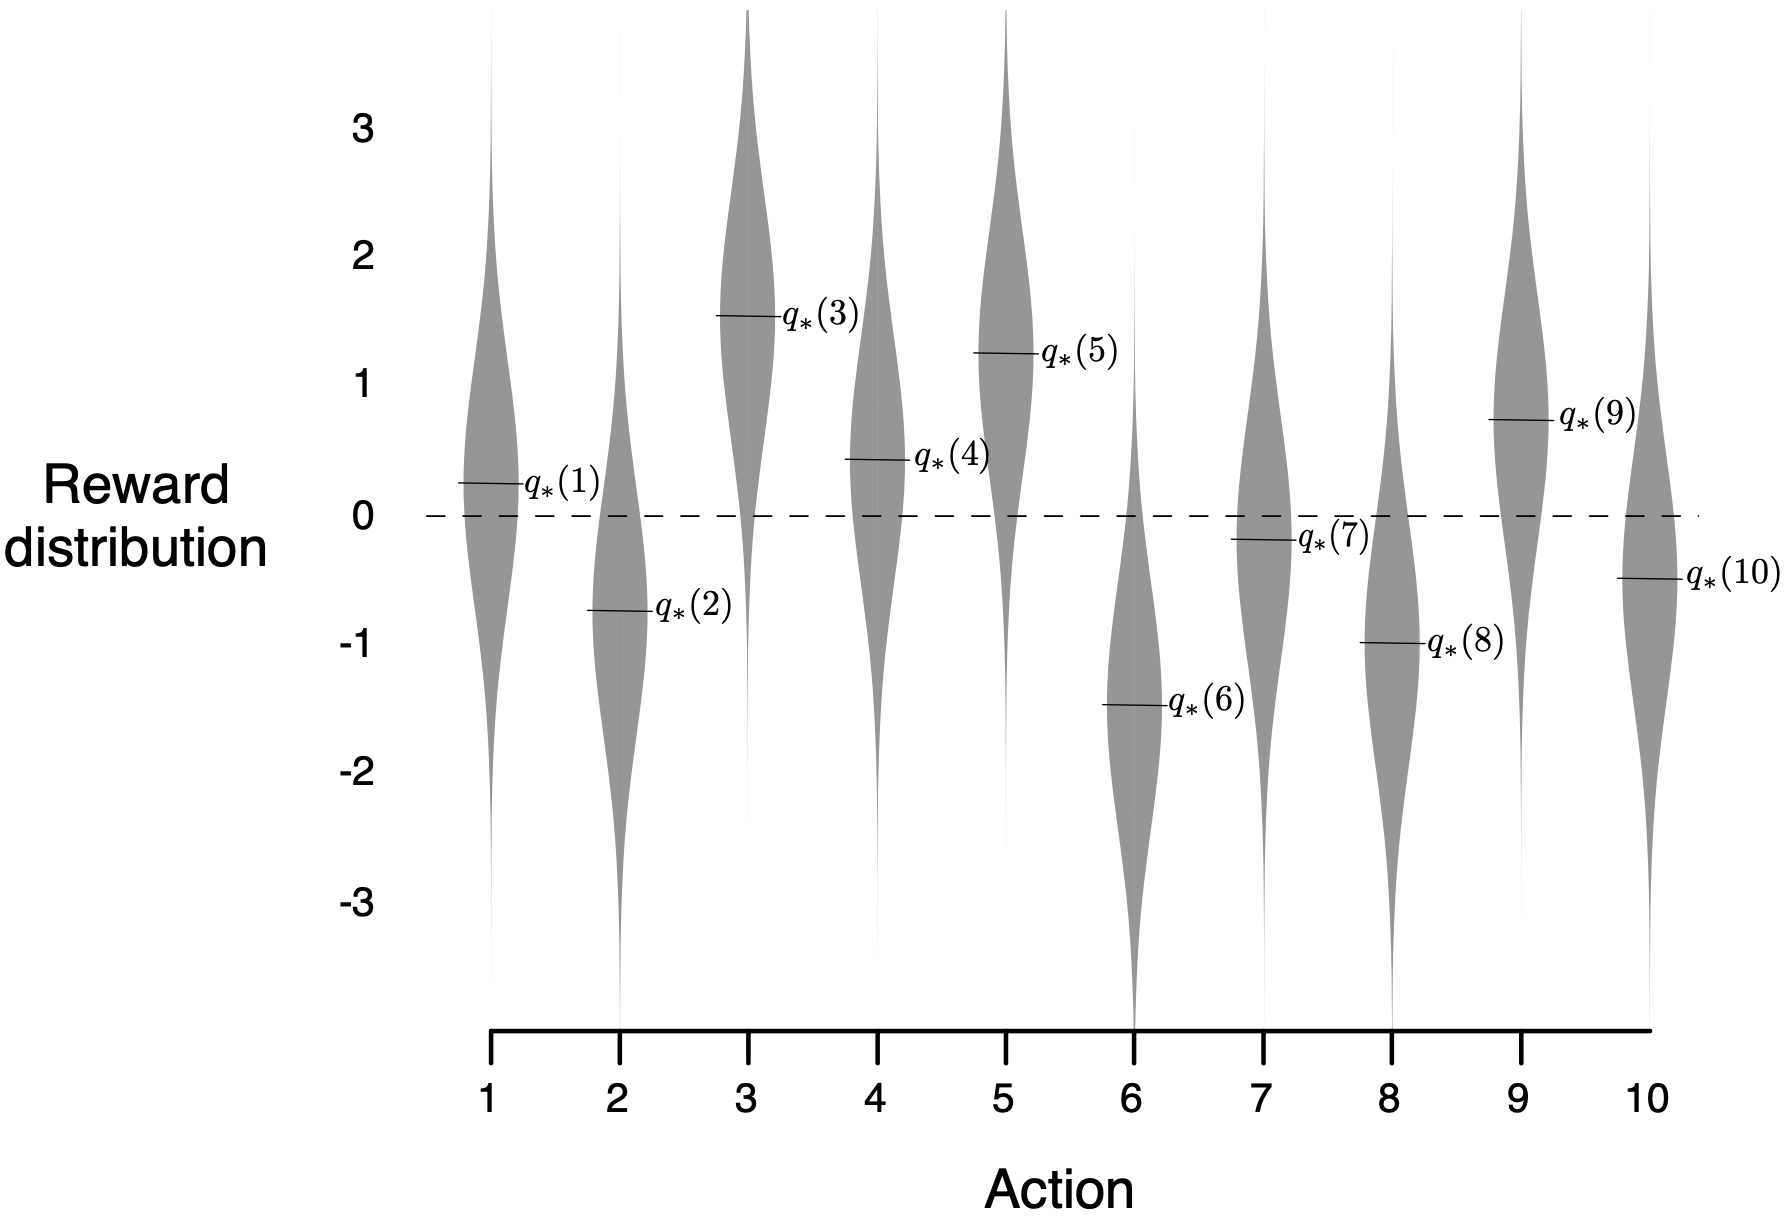
\includegraphics[width=0.9\columnwidth]{images/10-armed-eg1.png}
    \caption{10-armed testbed}
    \label{fig:fig1}
\end{figure}

\begin{itemize}
\item
  \textbf{Figure \ref{fig:fig1}:} An example bandit problem from the 10-armed
  testbed. The true value \(q_*(a)\) of each of the ten actions was
  selected according to a normal distribution with mean zero and unit
  variance, and then the actual rewards were selected according to a
  mean \(q_*(a)\) unit variance normal distribution, as suggested by
  these gray distributions.
\end{itemize}

\begin{itemize}
\item
  Then compares a greedy method with two \(\epsilon\)-greedy methods
  (\(\epsilon = 0.01\) and \(\epsilon = 0.1\)):
\end{itemize}


\begin{figure}[H]
  \centering  % Remember to centre the figure
    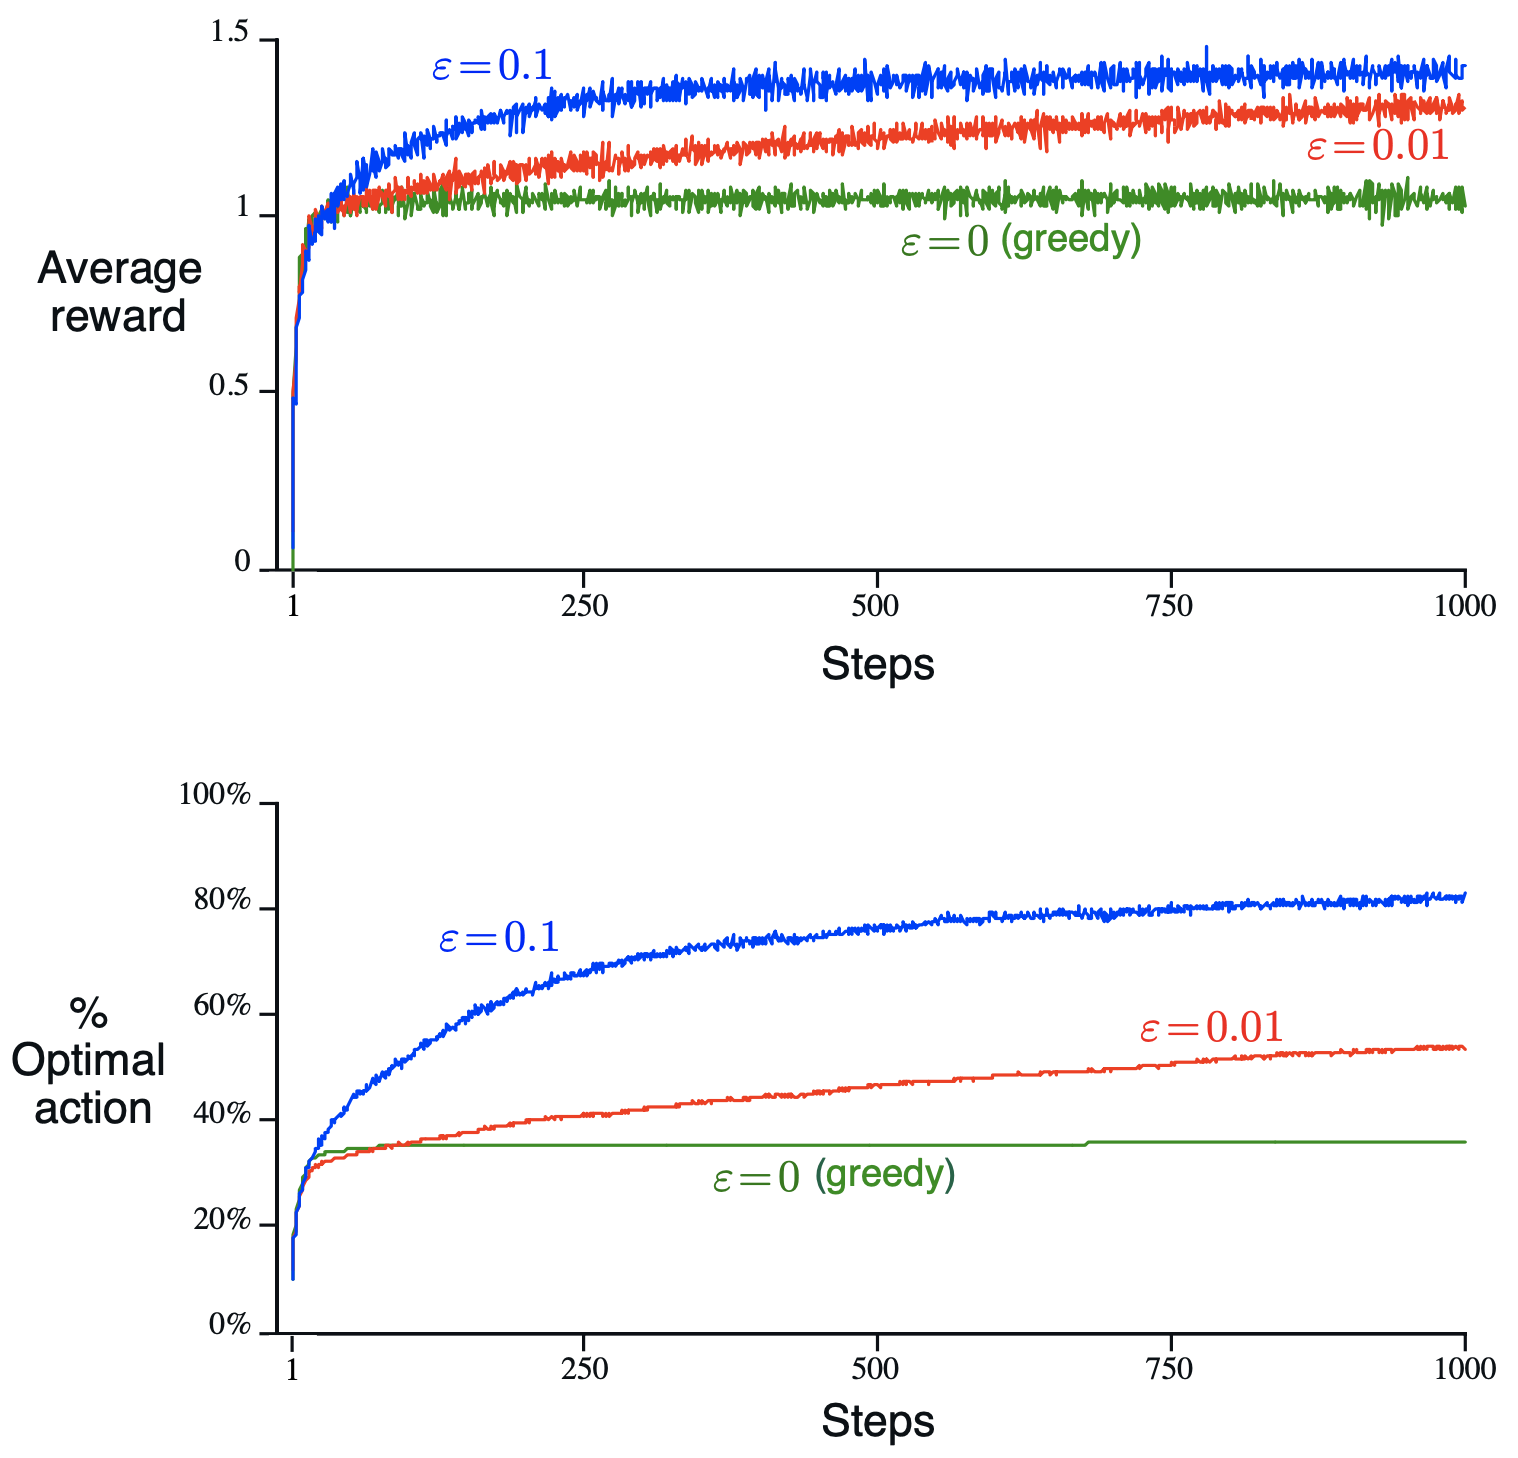
\includegraphics[width=0.9\columnwidth]{images/10-armed-eg2.png}
    \caption{Average performance of \(\epsilon\)-greedy action-value methods on the 10-armed testbed}
    \label{fig:fig2}
\end{figure}


\begin{itemize}
\item
  \textbf{Figure \ref{fig:fig2}:} Average performance of \(\epsilon\)-greedy
  action-value methods on the 10-armed testbed. These data are averages
  over 2000 runs with different bandit problems. All methods used sample
  averages as their action-value estimates.
\end{itemize}

\begin{itemize}
\item
  NOTE:

  \begin{itemize}
  \item
    The \(\epsilon = 0.01\) method improved more slowly, but eventually
    would perform better than the \(\epsilon = 0.1\) method on both
    performance measures shown in the figure.
  \item
    It is \textbf{also possible} to reduce \(\epsilon\) over time to try
    to get the best of both high and low \(\epsilon\) values.
  \item
    With \textbf{noisier rewards} it takes more exploration to find the
    optimal action.
  \end{itemize}
\end{itemize}

\textbf{Exploration} is beneficial even in the deterministic worlds
\textbf{if:}
\begin{itemize}
  \item \textbf{nonstationary} task, that is, the \textbf{true
  values of the actions changed over time} \(\rightarrow\) \textbf{agent's
  decision-making policy changes}.
  \item \textbf{nonstationary} is the case most commonly encountered in reinforcement learning.
\end{itemize}

\textbf{Example:} A simple bandit algorithm

Pseudocode for a complete bandit algorithm using incrementally computed
sample averages and \(\epsilon\)-greedy action selection is shown in the
box below.

\begin{tcolorbox}
  \textbf{Initialize, for \(a = 1 \; to \; k\):} \(\;\;\;\)
  \(Q(a) \leftarrow 0\) \(\;\;\;\) \(N(a) \leftarrow 0\)

  \textbf{Loop forever:}
  $$\;\;\; A \leftarrow \begin{cases} \argmax_{a}Q(a) &\texttt{with probability } 1- \epsilon \;\;\; \texttt{(breaking ties randomly)} \\ \texttt{random action} &\texttt{with probability } \epsilon \end{cases}$$
  $$\;\;\; R \leftarrow bandit(A)$$
  $$\;\;\; N(a) \leftarrow N(a)+1$$
  $$\;\;\; Q(A) \leftarrow Q(A) + \frac{1}{N(A)}[R-Q(A)]$$
\end{tcolorbox}

\begin{itemize}
\item
  Where:

  \begin{itemize}
  \item
    \textbf{function \(bandit(a)\)} is assumed to \textbf{take} an
    action and \textbf{return} a corresponding reward
  \end{itemize}
\end{itemize}









\subsection{Tracking a Nonstationary Problem}\label{tracking-nonstationary-problem}

\textbf{What:} true values of the actions changed over time
\(\rightarrow\) agent's decision-making policy changes.

\textbf{Adjustments:} it makes sense to give more weight to recent
rewards than to long-past rewards.

\begin{itemize}
\item
  A \textbf{POPULAR WAY} it to use a \textbf{constant step-size
  parameter \(\alpha\)} (2.3 modified to be):
\end{itemize}

\begin{gather*}
  Q_{n+1} = Q_n + \alpha [R_n - Q_n] \\ \\
  \textbf{Where:} \\
  \alpha \in (0,1]\ \text{: is constant} \\
\end{gather*}


\textbf{\(\rightarrow\) resulting in \(Q_{n+1}\) being a weighted
average of past rewards and the initial estimate \(Q_1\)} (sometimes
called an \emph{exponential recency-weighted average}):

\[Q_{n+1} = (1 - \alpha )^n Q_1 + \sum_{i=1}^n \alpha (1 - \alpha)^{n-1} R_i \;\;\;\;\;(2.6)\]

\begin{center}\rule{0.5\linewidth}{0.5pt}\end{center}











\subsection{Optimistic Initial Values}\label{optimistic-initial-values}


\textbf{What:} a common strategy of balancing exploration-exploitation.

\textbf{How:} encouraging early exploration with optimistic initial values for all possible actions.

\textbf{Limitations:}
\begin{itemize}
  \item \textcolor{red}{Drive only early exploration}
  \item \textcolor{red}{Not well-suitable for} non-stationary problems
  \item \textcolor{red}{We may not always know how to set the optimistic initial values}, because in practice we may not know the maximal reward.
\end{itemize}














% =============== CHAPTER 3 - Finite Markov Decision Processes ===============



\section{Finite Markov Decision Processes}\label{finite-markov-decision-processes}

\textbf{Markov decision process (MDP)} provides a \uline{mathematical framework
for modeling sequential decision-making in situations where outcomes are partly
random and partly under the control of a decision maker}.

A \textbf{MDP is a 4-tuple \((S,A,p,R)\)}, where:

\begin{itemize}
\item
  \(S\) is a set of states called the state space,
\item
  \(A\) is a set of actions called the action space (alternatively,
  \(A(s)\) is the set of actions available from state \(s\)),
\item
  \(p(s', r|s, a) = Pr\{S_t = s', R_t =r | S_{t-1} = s, A_{t-1} = a\}\)
  is the probability that action \(a\) in state \(s\) at time \(t\) will
  lead to state \(s'\) at time \(t+1\),
\item
  \(R_{a}(s,s')\) is the immediate reward (or expected immediate reward)
  received after transitioning from state \(s\) to state \(s'\), due to
  action \(a\)
\end{itemize}

The state and action spaces may be \textbf{finite} or \textbf{infinite}:

\begin{itemize}
  \item e.g. the set of real numbers is infinite.
  \item Some processes with
  countably infinite state and action spaces can be reduced to ones with
  finite state and action spaces.
\end{itemize}

A \textbf{policy function \(\pi\)} is a (potentially probabilistic)
mapping from state space to action space.

\textbf{Optimization objective} \(\rightarrow\) find a good ``policy''
for the decision maker.

\begin{itemize}
  \item \textbf{EXTRA:} Once a MDP is \textbf{combined
  with} a policy in this way, this fixes the action for each state and the
  resulting combination \textbf{behaves like a Markov chain} (since the
  action chosen in state \(s\) is completely determined by \(\pi(s)\) and
  \(\Pr(s_{t+1}=s'\mid s_{t}=s,a_{t}=a)\) reduces to
  \(\Pr(s_{t+1}=s'\mid s_{t}=s)\), a \textbf{Markov transition matrix}).
\end{itemize}






\subsection{The Agent--Environment Interface }\label{agent-environment-interface}

\textbf{Agent:} learner and decision maker.

\textbf{Environment:} thing agent interacts with, comprising everything
outside the agent.

The environment also gives rise to \textbf{rewards}, special numerical
values that the agent seeks to maximize over time through its choice of
\textbf{actions}.


\begin{figure}[H]
  \centering  % Remember to centre the figure
    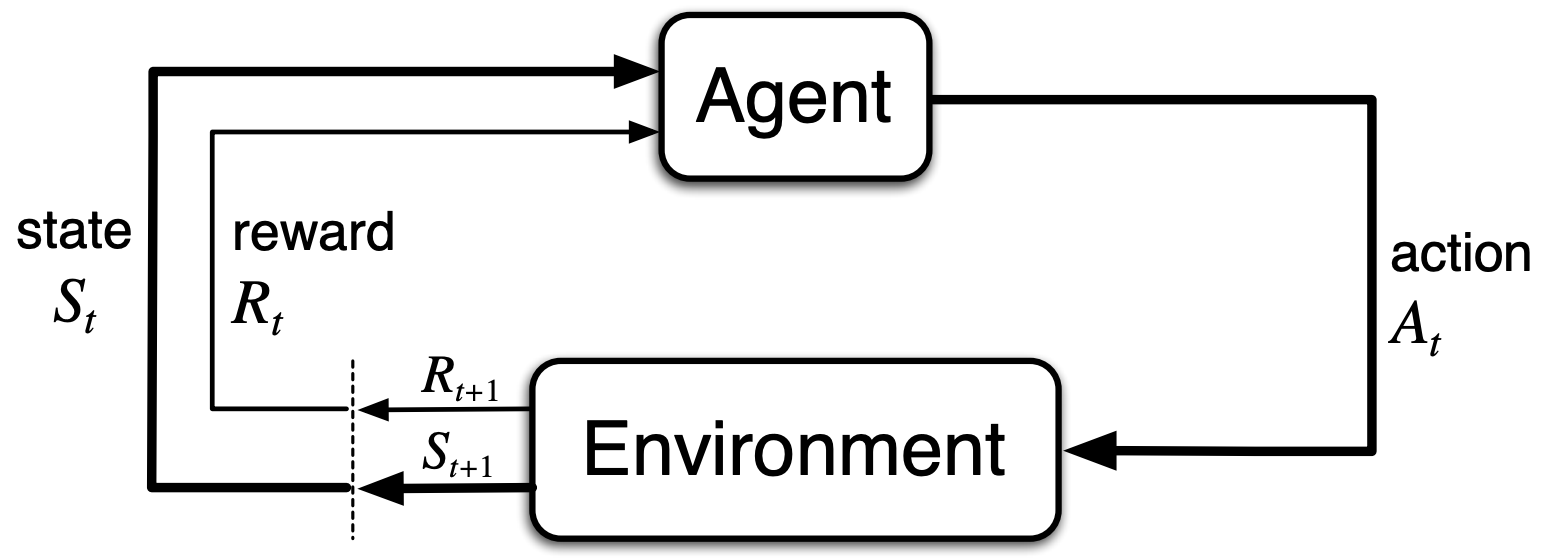
\includegraphics[width=0.9\columnwidth]{images/MDP-agent-environment-interaction.png}
    \caption{MDP agent-environment interaction}
    \label{fig:fig3}
\end{figure}


The MDP and agent together give rise to a \emph{sequence} or
\emph{trajectory} that begins like this:

\[S_0, A_0, R_1, S_1, A_1, R_2, S_2, A_2, R_3,... \]

\emph{In general}, \textbf{actions} can be any decisions we want to
learn how to make, and the \textbf{states} can be anything we can know
that might be useful in making them.

In a \textbf{finite MDP}, the sets of states, actions, and rewards
(\(S\), \(A\), and \(R\)) all have a finite number of elements.

In this case, the \textbf{random variables \(R_t\) and \(S_t\)} have
well defined discrete probability distributions \textbf{dependent only
on} the preceding state and action.

There is a \textbf{probability of those values occurring at time t},
given particular values of the preceding state and action:

\[p(s', r|s, a) = Pr\{S_t = s', R_t =r | S_{t-1} = s, A_{t-1} = a\},\]

Where:

\begin{itemize}
\item
  \(s' =\) particular values of the random variable \(S\) (\(s' \in S\))
\item
  \(r =\) particular values of the random variable \(R\) (\(r \in R\))
\end{itemize}

The \textbf{function \(p\)} defines the dynamics of the MDP. \(p\)
specifies a probability distribution for each choice of \(s\) and \(a\).

Total probability is thus:

\[\sum_{s' \in S} \sum_{r \in R} p(s', r|s, a) = 1, for\;all\;s \in S, a \in A(s)\]

\textbf{Markov property:} The state must include information about all
aspects of the past agent--environment interaction that make a
difference for the future.

\begin{itemize}
  \item (only present matters)
  \item (things/rules/transition model are stationary)
  \item We will assume the
  Markov property throughout this book.
\end{itemize}


\textbf{Calculations from the four-argument dynamics function:}

\begin{itemize}
\item
  \textbf{state-transition probabilities
  \(p : S \times S \times A \rightarrow [0, 1]\)}

  \begin{itemize}
  \item
    \(p(s'|s, a) = Pr\{S_t = s'| S_{t-1} = s, A_{t-1} = a\} = \sum_{r \in R} p(s', r|s, a)\)
  \end{itemize}
\item
  \textbf{expected rewards for state--action pairs
  \(r : S \times A \rightarrow \mathbb{R}\)}

  \begin{itemize}
  \item
    \(r(s,a) = E[R_t | S_{t-1}=s, A_{t-1}=a] = \sum_{r \in R} \sum_{s' \in S} p(s', r|s, a)\)
  \end{itemize}
\item
  \textbf{expected rewards for state--action--next-state triples
  \(r : S \times A \times S \rightarrow \mathbb{R}\)}

  \begin{itemize}
  \item
    \(r(s,a, s') = E[R_t | S_{t-1}=s, A_{t-1}=a, S_t = s'] = \sum_{r \in R} r \frac{p(s', r | s, a)}{p(s' | s, a)}\)
  \end{itemize}
\end{itemize}









\subsection{Goals and Rewards}\label{goals-and-rewards}

\textbf{Reward Hypothesis:}

\begin{itemize}
\item
  That all of what we mean by \textbf{goals $G$} and purposes \emph{can be well thought of as} the \uline{maximization of the expected value of the cumulative sum of a received scalar signal (called reward)}.
\end{itemize}

It is critical that the rewards we set up truly indicate what we want
accomplished.

\begin{itemize}
  \item \textbf{For example}, a chess-playing agent should be
  rewarded only for actually winning, not for achieving subgoals such as
  taking its opponent's pieces or gaining control of the center of the
  board. If achieving these sorts of subgoals were rewarded, then the
  agent might find a way to achieve them without achieving the real goal.
\end{itemize}

\textbf{Reward signal} is your way of communicating to the robot what
you want it to achieve, not how you want it achieved.







\subsection{Returns and Episodes }\label{returns-and-episodes}

In general, we seek to maximize the expected \textbf{return}, where the
return, denoted \(G_t\).

\textbf{Episodic Tasks}\label{episodic-tasks}

\(G_t\) is in the simplest case the \textbf{return} of the sum of the
rewards:

\[G_t \dot{=} R_{t+1} + R_{t+2} + R_{t+3} + ... + R_T \;\;\;\;\;(3.7)\]

Tasks with \emph{episodes} of this kind are called \textbf{episodic
tasks}. In episodic tasks we \textbf{sometimes need to distinguish} the
set of all nonterminal states, denoted \(S\), from the set of all states
plus the terminal state, denoted \(S^+\). The time of termination,
\(T\), is a random variable that normally varies from episode to
episode.


\textbf{Continuing Tasks}\label{continuing-tasks}


On the other hand, in many cases the agent--environment interaction does
not break naturally into identifiable episodes, but goes on
\textbf{continually without limit}. We call these \textbf{continuing
tasks}.

In this book we usually use a definition of return that is slightly more
complex conceptually but much simpler mathematically. The additional
concept that we need is that of \textbf{discounting}. According to this
approach, the agent tries to select actions so that the sum of the
discounted rewards it receives over the future is maximized. In
particular, it chooses \(A_t\) to maximize the expected discounted
return:

\[G_t = R_{t+1} + \gamma R_{t+2} + \gamma^2 R_{t+3} + ... = \sum_{k=0}^{\infty} \gamma^k R_{t+k+1} \;\;\;\;\;(3.8)\]

Where:

\begin{itemize}
\item
  \(\gamma =\) is a parameter, \(0 \leq \gamma \leq 1\), called the
  \textbf{discount rate}.

  \begin{itemize}
  \item
    If \(\gamma < 1\), the infinite sum has a finite value as long as
    the reward sequence \(\{R_k\}\) is bounded.
  \item
    If \(\gamma = 0\), the agent is ``myopic'' in being concerned only
    with maximizing immediate rewards: its objective in this case is to
    learn how to choose \(A_t\) so as to maximize only \(R_{t+1}\). But
    in general, acting to maximize immediate reward can reduce access to
    future rewards so that the return is reduced.
  \item
    As \(\gamma\) approaches \(1\), the return objective takes future
    rewards into account more strongly; the agent becomes more
    farsighted.
    \begin{itemize}
      \item If $\gamma = 1$, undiscounted.
    \end{itemize}
  \end{itemize}
\end{itemize}

\textbf{Returns at successive time steps} are related to each other in a
way that is important for the theory and algorithms of reinforcement
learning:

\begin{align*}
  G_t &= R_{t+1} + \gamma R_{t+2} + \gamma^2 R_{t+3} + \gamma^3 R_{t+4} + ... \\
  &= R_{t+1} + \gamma (R_{t+2} + \gamma R_{t+3} + \gamma^2 R_{t+4} + ...)  \\
  &= R_{t+1} + \gamma G_{t+1} \\
\end{align*}

\begin{itemize}
\item
  Note that this works for all time steps \(t<T\), even if termination
  occurs at \(t + 1\), if we define \(G_T = 0\)
\item
  Note that although the return is a sum of an infinite number of terms,
  it is still finite if the reward is nonzero and constant, if
  \(\gamma < 1\).
\end{itemize}






\subsection{Unified Notation for Episodic and Continuing Tasks}
\label{unified-notation-for-episodic-and-continuing-tasks}

In the preceding section we described two kinds of reinforcement
learning tasks:

\begin{itemize}
\item
  \textbf{episodic tasks:} agent--environment interaction naturally
  breaks down into a sequence of separate episodes.
\item
  \textbf{continuing tasks:} agent--environment interaction don't breaks
  down into a sequence of separate episodes.
\end{itemize}

We have defined the return as a sum over a finite number of terms in one
case (3.7) and as a sum over an infinite number of terms in the other
(3.8). These two can be unified by considering \textbf{episode
termination} to be the entering of a \uline{special absorbing state that
transitions only to itself and that generates only rewards of zero}. For
example, consider the state transition diagram:


\begin{figure}[H]
  \centering  % Remember to centre the figure
    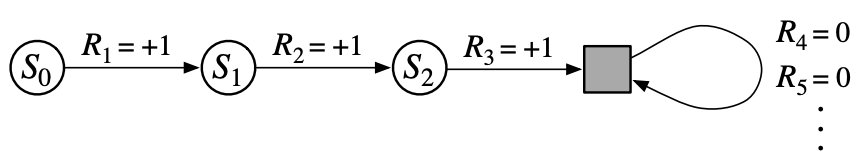
\includegraphics[width=0.9\columnwidth]{images/Unified-Notation-Episodic-and-Continuing-Tasks.png}
    \caption{State transition diagram}
    \label{fig:fig4}
\end{figure}


Starting from \(S_0\), we get the reward sequence
\(+1, +1, +1, 0, 0, 0,...\). Summing these, we get the same return
whether we sum over the first \(T\) rewards (here \(T = 3\)) or over the
full infinite sequence. This remains true even if we introduce
discounting.

Thus, we can define the \textbf{return, in general}, according to (3.8),
using the convention of omitting episode numbers when they are not
needed, and including the possibility that = 1 if the sum remains
defined (e.g., because all episodes terminate). Alternatively, we can
write:

\[G_t = \sum_{k=t+1}^T \gamma^{k-t-1} R_k\]

\begin{itemize}
\item
  including the possibility that \(T = \infty\) or \(\gamma = 1\) (but
  not both).
\end{itemize}







\subsection{Policies and Value Functions}\label{policies-and-value-functions}

Almost all \textbf{reinforcement learning algorithms involve estimating
\textcolor{blue}{value functions}} --- functions of states (or of state--action
pairs) that \uline{estimate how good it is for the agent to be in a given state} (or \uline{how good it is to perform a given action in a given state}). They allow an agent to query the quality of its current situation instead of waiting to observe the long-term outcome. Thus, \uline{\textbf{value functions} enable us to judge the quality of different \textbf{policies}}.

\begin{figure}[H]
  \centering  % Remember to centre the figure
    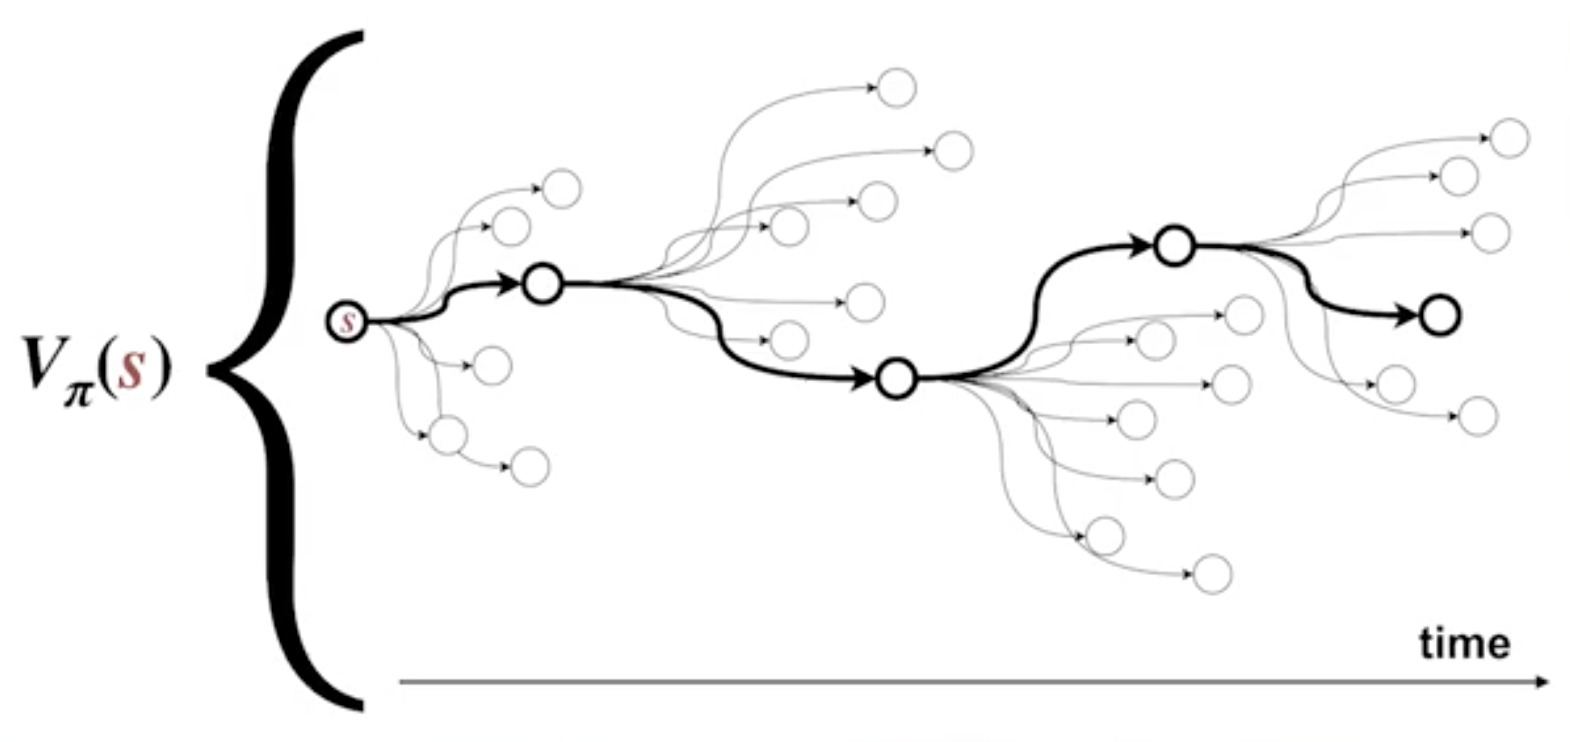
\includegraphics[width=0.8\columnwidth]{images/value-function-predicting-rewards.png}
    \caption{Illustration of value function predicting rewards into the future}
    \label{fig:value-function-predicting-rewards}
\end{figure}

\textcolor{blue}{\textbf{Policy \(\pi\)}} is a \uline{\textbf{mapping from} states \textbf{to} probabilities of selecting each possible action}. If the agent is
following policy \(\pi\) at time \(t\), then \(\pi(a|s)\) is the
probability that \(A_t = a\) if \(S_t = s\).

A policy by definition \uline{depends only on the current state}. It cannot depend on things like time or previous states. This is best thought of as a restriction on the state, not the agent. The state should provide the agent with all the information it needs to make a good decision.

\begin{itemize}
  \item Accordingly, value functions are defined with respect to particular ways of acting, called \textbf{policies}.
\end{itemize}

\begin{figure}[H]
  \centering  % Remember to centre the figure
    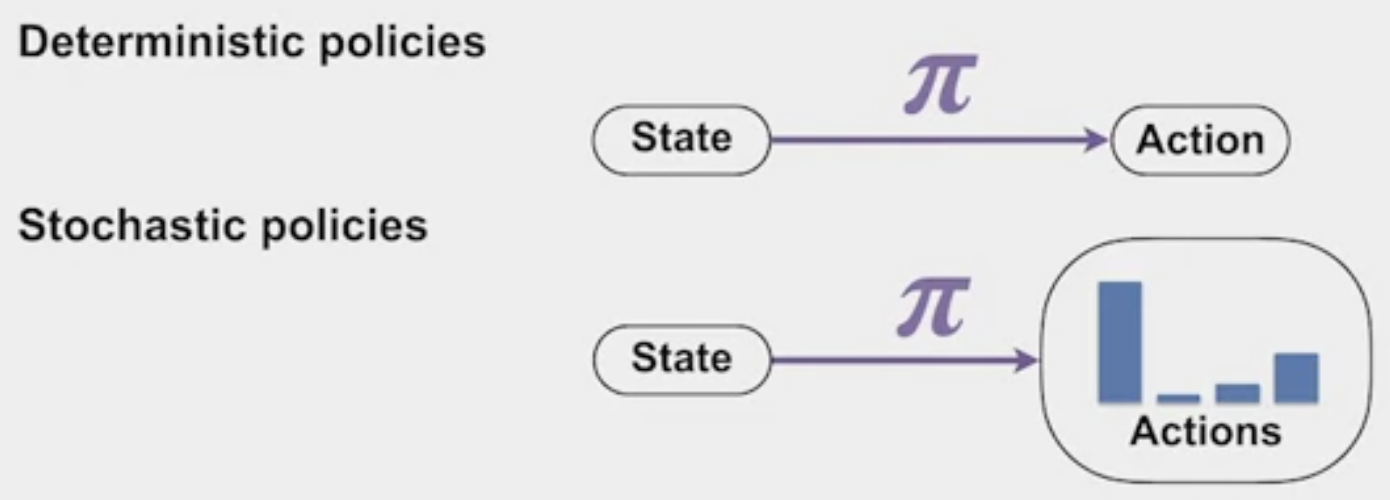
\includegraphics[width=0.8\columnwidth]{images/deterministic-and-stochastic-policies.png}
    \caption{Policies tell an agent how to behave in their environment}
    \label{fig:value-function-predicting-rewards}
\end{figure}

\textbf{Reinforcement learning methods specify} \uline{how the agent's policy is changed as a result of its experience}.

The \textcolor{blue}{\textbf{state-value functions \(v_\pi(s)\)}} of a state \(s\) under a policy \(\pi\), is the expected return when starting in \(s\) and following \(\pi\) thereafter. For MDPs, we can define \(v_\pi\) formally by

\[v_\pi(s) = E_\pi[G_t|S_t=s] = E_\pi[\sum_{k=0}^{\infty} \gamma^k R_{t+k+1} | S_t = s], for\;all\; s \in S \;\;\;\;\;(3.12)\]

Where:

\begin{itemize}
\item
  \(E_\pi[]\) denotes the expected value of a random variable given that
  the agent follows policy \(\pi\), and \(t\) is any time step.
\end{itemize}

The \textcolor{blue}{\textbf{action-value function \(q_\pi(s, a)\)}} for policy \(\pi\) is
defined as the \textbf{value of taking action \(a\) in state \(s\) under
a policy \(\pi\)}, as the expected return starting from \(s\), taking
the action \(a\), and thereafter following policy \(\pi\):

\[q_\pi(s, a) = E_\pi[G_t|S_t=s, A_t=a] = E_\pi[\sum_{k=0}^{\infty} \gamma^k R_{t+k+1} | S_t = s, A_t = a] \;\;\;\;\;(3.13)\]

A \textbf{fundamental property of value functions} used throughout
reinforcement learning and dynamic programming is that they satisfy
recursive relationships similar to that which we have already
established for the return (3.9).








\subsection{Optimal Policies and Value Functions}\label{optimal-policies-and-value-functions}

\textcolor{Green}{\textbf{Solving a reinforcement learning task}} means, roughly, finding a policy that achieves a lot of reward over the long run.

For finite MDPs, we can precisely define an \textcolor{blue}{\textbf{optimal policy \(\pi_*\)}} as follows: * \(\pi \geq \pi'\) if and only if
\(v_\pi(s) \geq v_{\pi'}(s)\) for all \(s \in S\) * \textbf{Always at
least one policy} that is better than or equal to all other policies.


\begin{figure}[H]
  \centering  % Remember to centre the figure
    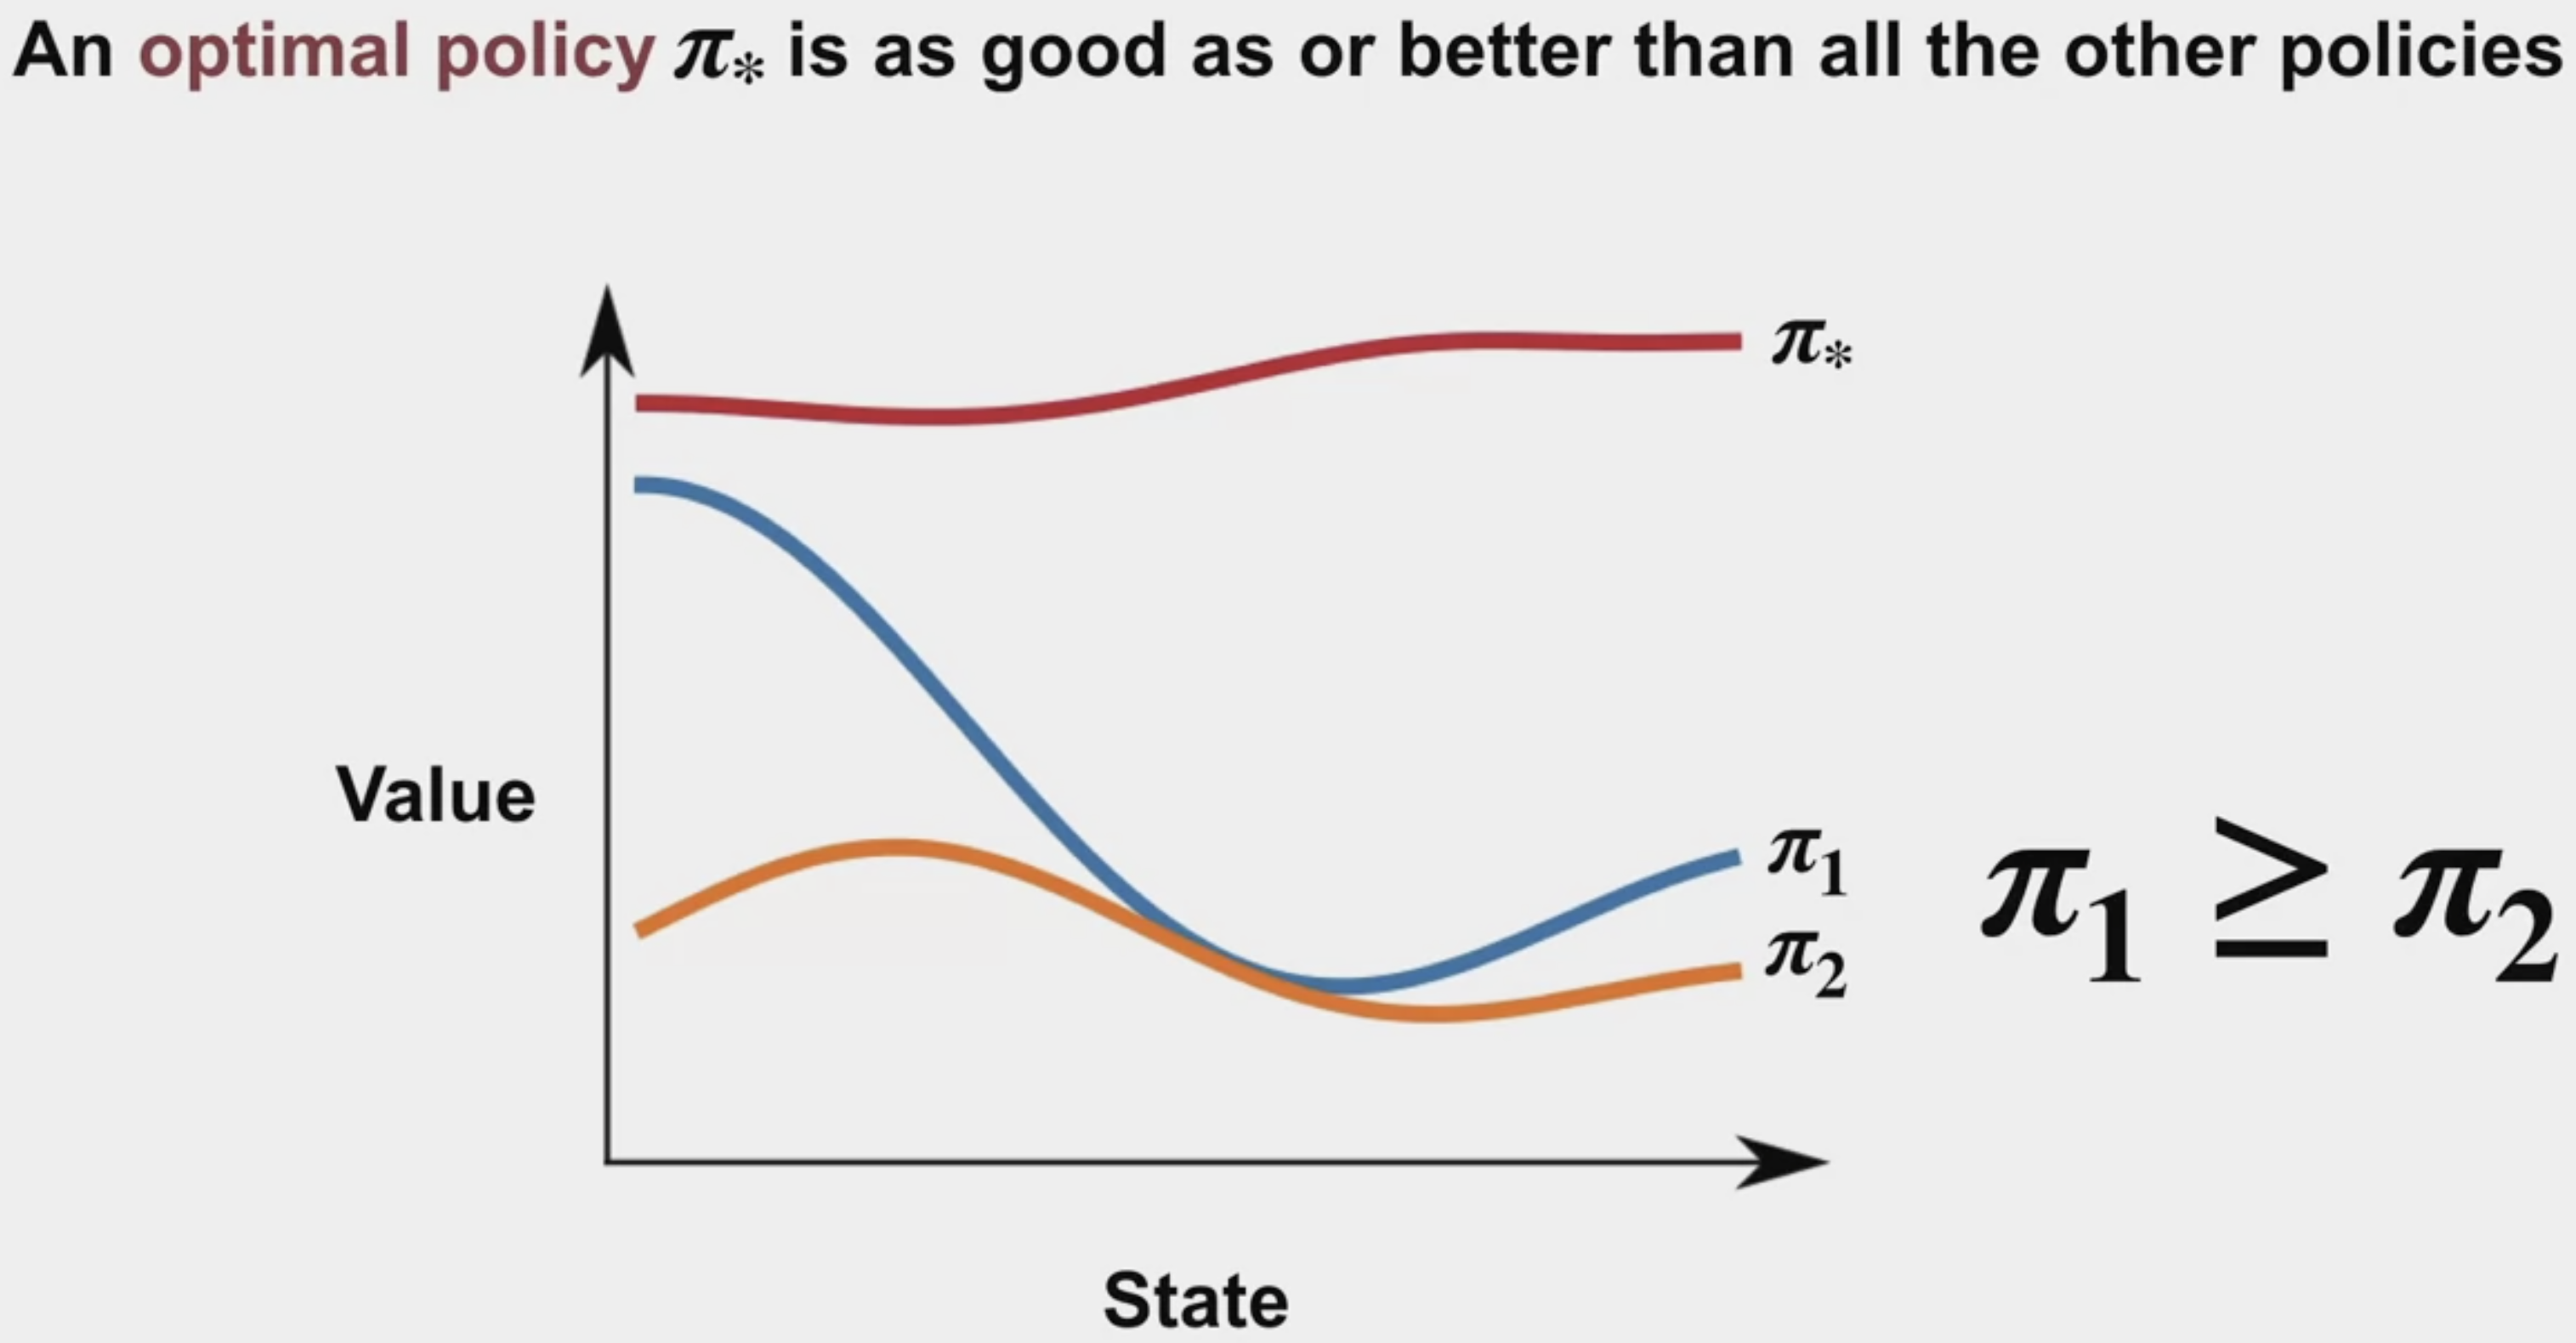
\includegraphics[width=0.8\columnwidth]{images/optimal-policy-eg.png}
    \caption{Illustration of optimal policy}
    \label{fig:optimal-policy-eg}
\end{figure}

How to find an optimal policy:
\begin{itemize}
  \item Once we had the \uline{optimal state value function}, it's relatively easy to work out the optimal policy.
  \item If we have the \uline{optimal action value function}, working out the optimal policy is even easier.
\end{itemize}

All optimal policies share the same \textcolor{blue}{\textbf{optimal state-value function
\(v_*\)}} defined as:

\[v_*(s) = \max_\pi v_\pi(s) \;for\;all\; s \in S \;\;\;\;\;\;(3.15)\]

Optimal policies also share the same \textcolor{blue}{\textbf{optimal action-value function \(q_*\)}} defined as:

\[q_*(s, a) = \max_\pi q_\pi(s, a) \;for\;all\; s \in S \; \& \; a \in A(s) \;\;\;\;\;\;(3.16)\]

For the state--action pair \((s, a)\), this function gives the expected
return for taking action \(a\) in state \(s\) and thereafter following
an optimal policy. Thus, we can write \textbf{\(q_*\) in terms of
\(v_*\)} as follows \textbf{(Bellman equation)}:

\[q_*(s, a) = E[R_{t+1} + \gamma v_*(S_{t+1}) | S_t = s, A_t = a] \;\;\;\;\;\;(3.17)\]






\subsection{Optimality and Approximation }\label{optimality-and-approximation}

For the kinds of tasks in which we are interested, \textcolor{red}{optimal policies can be generated only with extreme computational cost}. In particular, the amount of computation it can perform in a single time step.







\subsection{Why Bellman equations}\label{why-bellman-equations}

\textcolor{blue}{\textbf{Bellman equations}} define a \textbf{relationship between} the \uline{value of a state} or state-action pair and its \uline{possible successor states}.


Consider:

\begin{itemize}
  \item \textbf{Environment:}
  \begin{itemize}
    \item 4 states (A, B, C, D) in a square gridworld
    \item 25\% probability of moving (up, down, left or right)
    \begin{itemize}
      \item bumping into a border will result into staying in the current state
    \end{itemize}
  \end{itemize}
  \item \textbf{Policy:} Uniform random policy
  \item \textbf{Rewards:} The reward is 0 everywhere except for any time the agent lands in state B, the reward is +5.
  \item \textbf{Discoun factor $\gamma$:} 0.7
\end{itemize}

For the given setup, we can write value functions for each of the states (A, B, C, D) in form of Bellman equations:

\begin{figure}[H]
  \centering  % Remember to centre the figure
    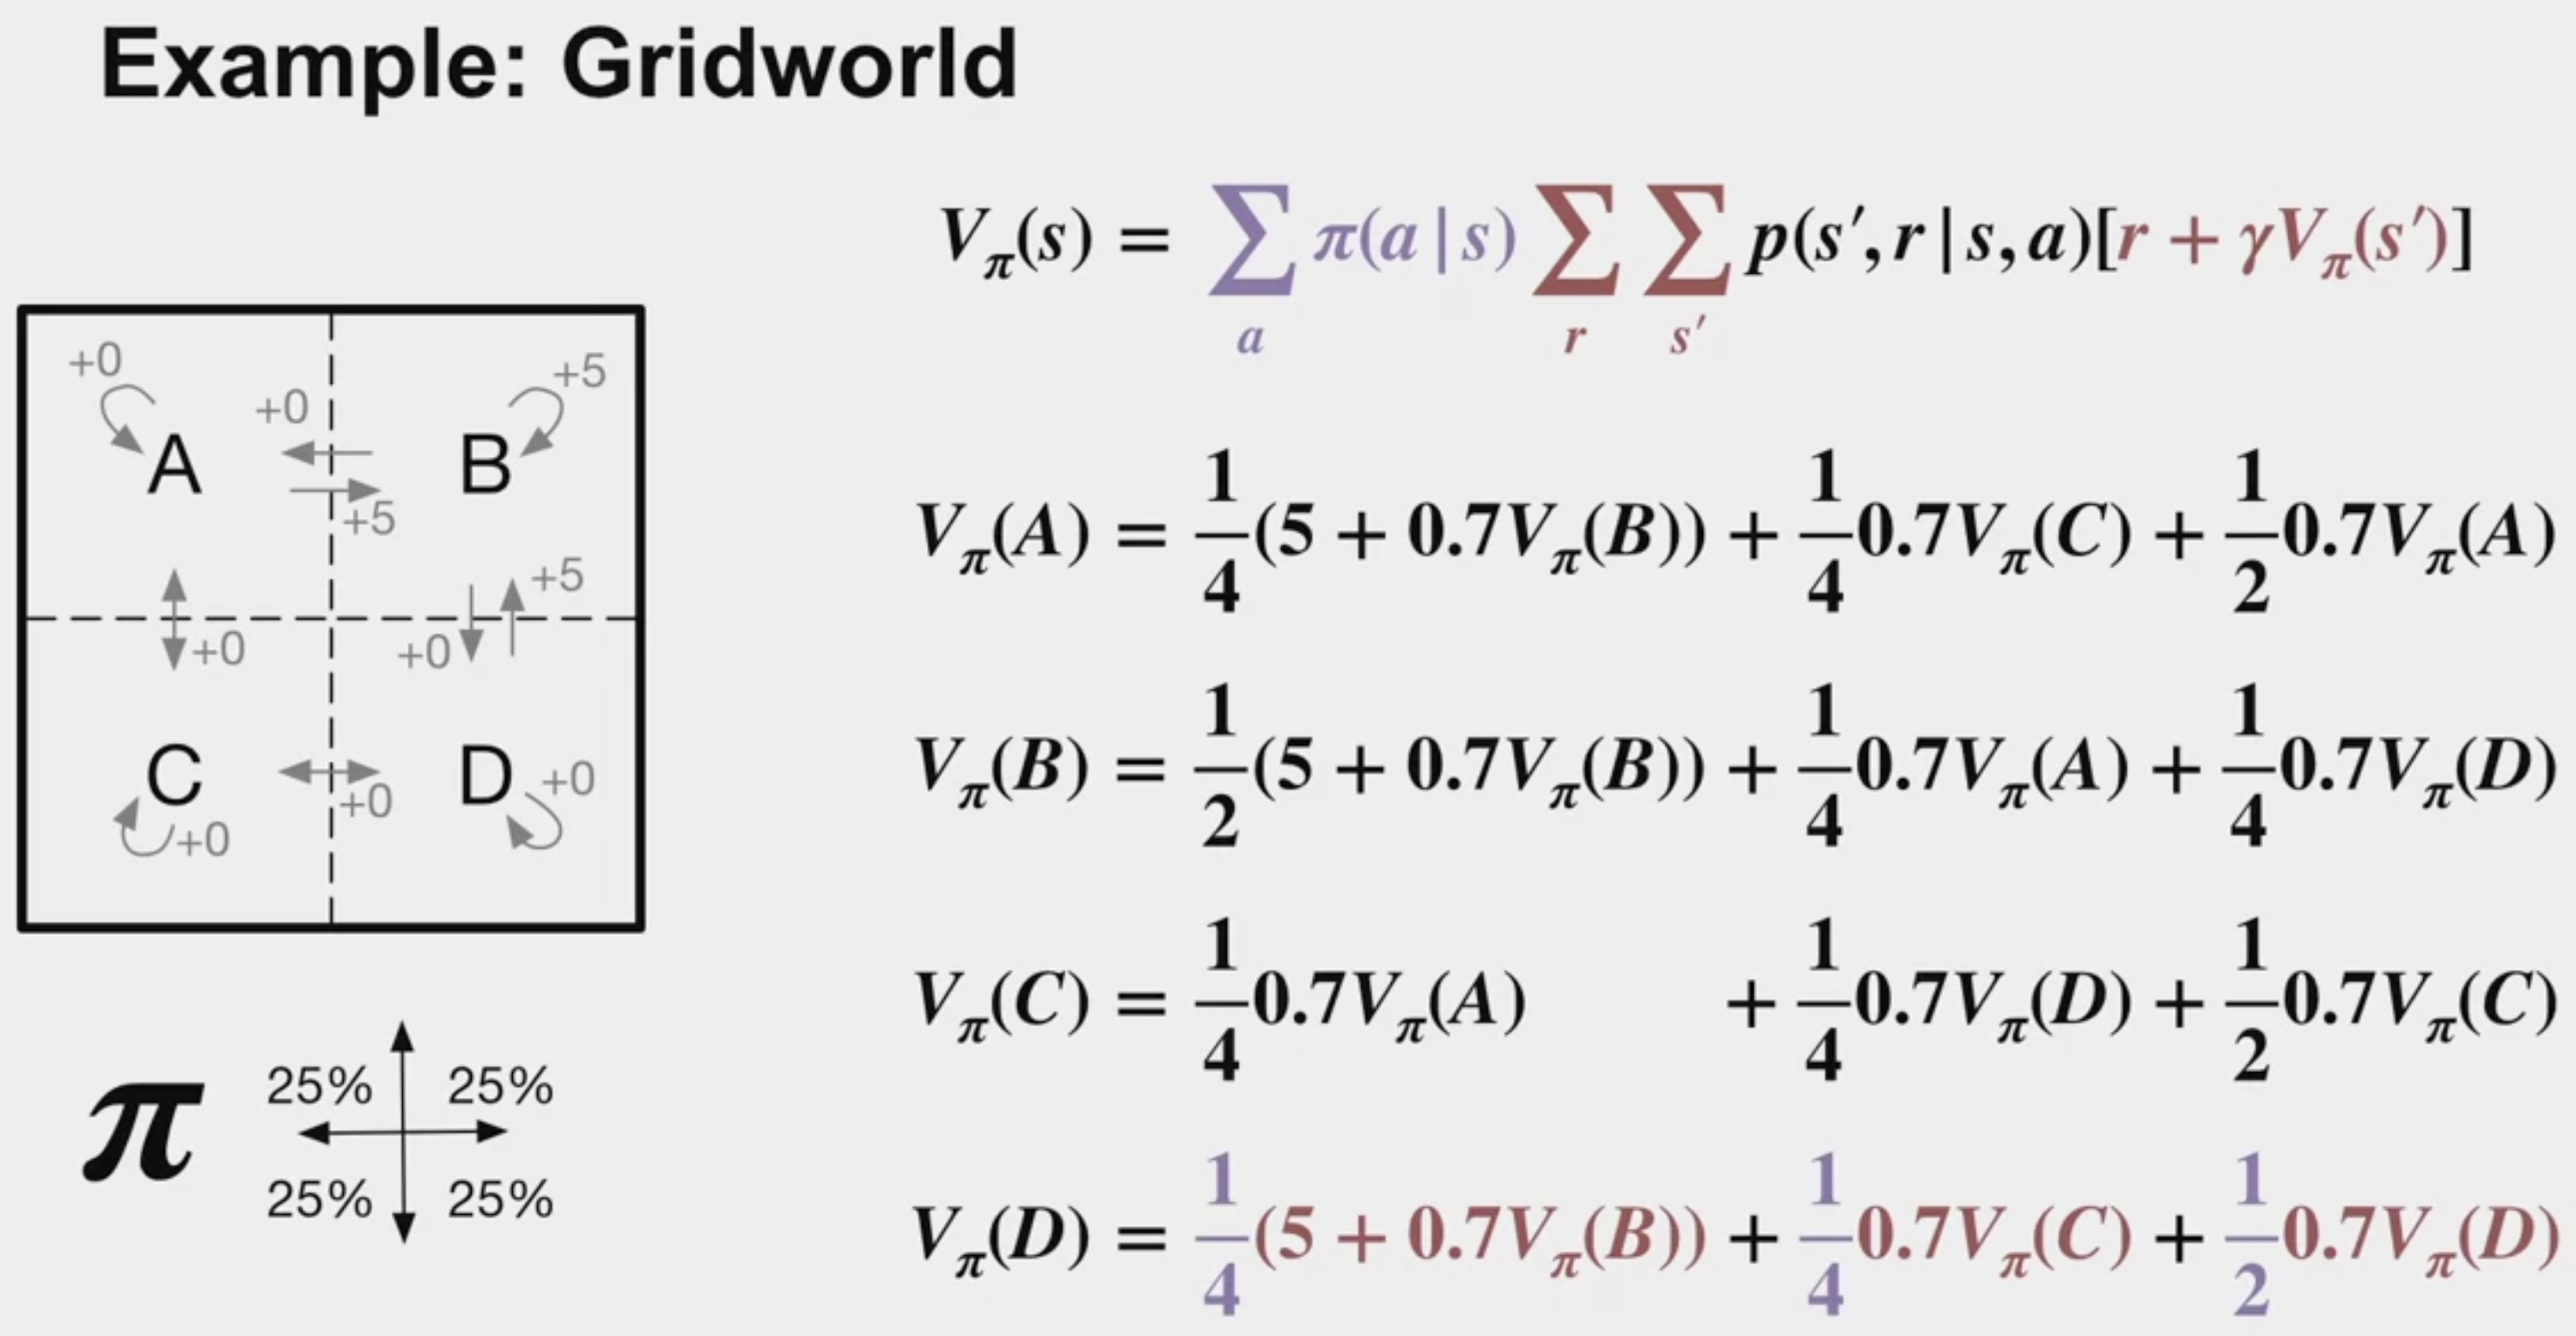
\includegraphics[width=0.9\columnwidth]{images/gridworld-eg.png}
    \caption{Value functions for all gridworld states}
    \label{fig:gridworld-eg}
\end{figure}
\begin{itemize}
  \item \textbf{Unique solutions to the Bellman equations:}
  \begin{itemize}
    \item $V_\pi(A) = 4.2$
    \item $V_\pi(B) = 6.1$
    \item $V_\pi(C) = 2.2$
    \item $V_\pi(D) = 4.2$
  \end{itemize}
\end{itemize}

The \textbf{important thing to note} is that the \uline{Bellman equation reduced an unmanageable infinite sum over possible futures, to a simple linear algebra problem}.

In this case we used the \textbf{Bellman equation} \uline{to directly write down a system of equations for the state values, and then some the system to find the values}. This approach may be possible for MDPs of moderate size. However, \textcolor{Red}{in more complex problems, this won't always be practical}.

\begin{itemize}
  \item e.g. Consider the game of chess for example. We probably won't be able to even list all the possible states, there are around 10 to the 45 of them.

  \begin{figure}[H]
    \centering  % Remember to centre the figure
      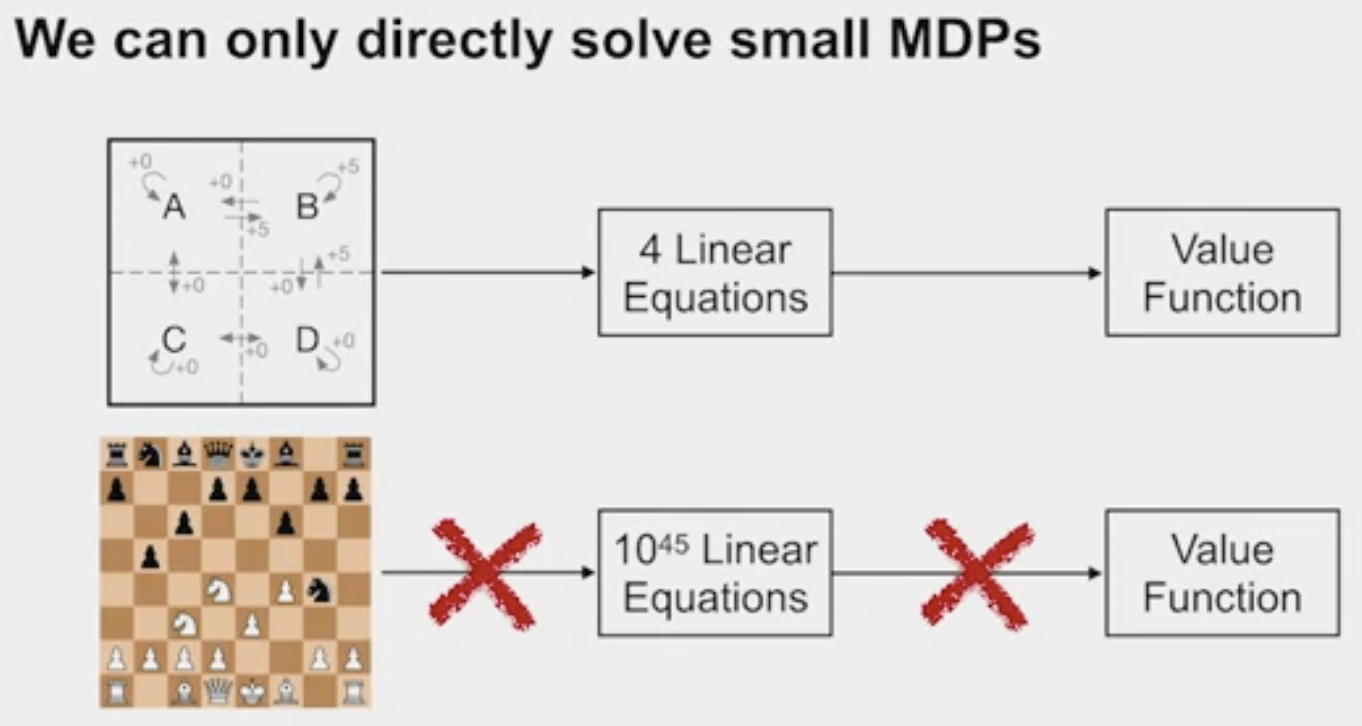
\includegraphics[width=0.8\columnwidth]{images/gridworld-eg2.png}
      \caption{Illustration how directly solving MDPs gets quickly problematic}
      \label{fig:gridworld-eg}
  \end{figure}

\end{itemize}




\subsection{Summary}\label{summary}

\textcolor{Green}{\textbf{Solving a reinforcement learning task}} means, roughly, finding a policy that achieves a lot of reward over the long run.

The \textbf{first step in applying reinforcement learning} will always be to \uline{formulate the problem as an MDP}.

\textcolor{blue}{\textbf{Markov property:}} The state must include information about all aspects of the past agent--environment interaction that make a
difference for the future.
\begin{itemize}
  \item (only present matters)
  \item (things/rules/transition model are stationary)
  \item We will assume the
  Markov property throughout this book.
\end{itemize}

\textcolor{blue}{\textbf{Policy \(\pi\), \(\pi(a|s)\):}} action to take for any given
state

\begin{itemize}
  \item Any policy: \(\pi(s) \rightarrow a\)
  \item Optimal policy:
  \(\pi^*(s) \rightarrow a\) * maximizes long-term expected reward
\end{itemize}


\textcolor{blue}{\textbf{State-Value functions \(v_\pi(s)\):}} expected cumulative rewards
when starting in \(s\) and following policy \(\pi\) thereafter.

\begin{itemize}
  \item or MDPs, we can define \(v_\pi\) formally by
  $$v_\pi(s) = E_\pi[G_t|S_t=s]$$

  \item \textbf{State-Value functions \(v_\pi(s)\):} can be decomposed into \textbf{immediate} and \textbf{future} components using \textcolor{blue}{\textbf{Bellman equation}}. Bellman equation forms the basis of a number of ways to compute, approximate, and learn \(v_\pi\).
  \begin{align*}
  V(s) &= E[G_t | s_t = s] \\
  V(s) &= E[r_{t+1} + \gamma V(s_{t+1} | s_t = s)] \\
  \end{align*}
  \begin{gather*}
    \textbf{Where:} \\
    \gamma =: \text{ is a parameter, \(0 \leq \gamma \leq 1\), called the
    \textbf{discount rate}.} \\
    \text{When \(0\) \(\rightarrow\) consider only
    immediate rewards} \\
    \text{When approaches \(1 \rightarrow\) forward looking}
  \end{gather*}
\end{itemize}

\textcolor{blue}{\textbf{Action-Value functions \(q_\pi(s, a), Q_\pi\):}} expected cumulative reward of taking action \(a\) when starting in \(s\) and
following policy \(\pi\) thereafter.
$$q_\pi(a) = E[R_t | A_t = a]$$

\begin{itemize}
  \item \textbf{Action-Value functions \(v_\pi(s)\):} can also be decomposed
  into \textbf{immediate} and \textbf{future} components using
  \textcolor{blue}{\textbf{Bellman equation}}.
  $$Q_\pi(s,a) = E_\pi[r_t + \gamma Q_\pi (S_{t+1}, a_{t+1}) | s_t=s, a_t=a]$$
  $$Q_\pi(s,a) = \sum_{s'} T(s,a,s') r(s,a,s') + \gamma \sum_{s'}T(s,a,s')Q_\pi(s',\pi(s'))$$
\end{itemize}

\textcolor{blue}{\textbf{Return \(G\) \& Rewards \(R\):}} return is the total of rewards

\begin{itemize}
  \item \(R(s) =\) reward of \textbf{entering state \(s\)}
  \item \(R(s, a) =\) reward of \textbf{entering state \(s\)} \& \textbf{taking action \(a\)}
  \item \(R(s, a, s') =\) reward of \textbf{being in state \(s\)} \& \textbf{taking action \(a\)} \& \textbf{entering state \(s'\)}
\end{itemize}

\textcolor{blue}{\textbf{State \(S\):}} every state agent could be in

\begin{itemize}
  \item \(S =\) set of \textbf{nonterminal states}
  \begin{itemize}
    \item \(s' =\) particular values of the random variable \(S\) (\(s' \in S\))
  \end{itemize}
  \item \(S^+ =\) set of \textbf{terminal states}
\end{itemize}

\textcolor{blue}{\textbf{Actions \(A, A(s)\):}} every action agent could take

\textcolor{blue}{\textbf{Function \(p\) (a.k.a Model / Transition function):}} defines the
dynamics of the environment. \(p\) specifies a probability distribution
for each choice of \(s\) and \(a\).

\begin{itemize}
  \item \textbf{state-transition
  probabilities \(p : S \times S \times A \rightarrow [0, 1]\)}
  $$
  p(s'|s, a) = Pr\{S_t = s'| S_{t-1} = s, A_{t-1} = a\} = \sum_{r \in R} p(s', r|s, a)
  $$
\end{itemize}

\begin{center}\rule{0.5\linewidth}{0.5pt}\end{center}












% =============== CHAPTER 4 - Dynamic Programming ===============


\section{Dynamic Programming (DP)}\label{dynamic-programming}


\textbf{What:} refers to a \uline{collection of algorithms that can be used to }\textbf{\uline{compute optimal policies}}\uline{ given a perfect model of the environment as a Markov decision process (MDP)}.


Pros and cons:

\begin{itemize}
  \item \textbf{+} Well developed mathematically
  \begin{itemize}
    \item \textcolor{orange}{All methods can be viewed as attempts to achieve much the same effect as DP, only with less computation and without assuming a perfect model of the environment.}
  \end{itemize}
  \item \textbf{-} Require a complete and accurate model of the environment (access to the dynamics function $p$)
\end{itemize}


DP algorithms \textbf{use the \textcolor{blue}{Bellman equations} to define iterative algorithms} for both \textcolor{blue}{\uline{policy evaluation}} and \textcolor{blue}{\uline{policy control}}.




\subsection{Policy Evaluation vs. Policy Control}\label{policy-evaluation-vs-policy-control}

\textbf{What:}
\begin{itemize}
  \item \textbf{\textcolor{blue}{Policy Evaluation:}} the task of \uline{determining the value function $v_\pi$ for a specific policy $\pi$}
  \item \textbf{\textcolor{blue}{Policy Control:}} the task of \uline{improving an existing policy $\pi$} (until it's optimal $\pi_*$).
\end{itemize}

\textbf{Why:}
\begin{itemize}
  \item \textbf{\textcolor{blue}{Policy Evaluation:}} for assessing how good a policy is $\rightarrow$ (to improve it)
  \item \textbf{\textcolor{blue}{Policy Control:}} for finding the optimal policy (goal of reinforcement learning)
\end{itemize}



\subsection{Iterative Policy Evaluation (Prediction)}\label{policy-evaluation-prediction}

\textbf{What:} \uline{\textbf{In \textcolor{blue}{DP}} we can do \textbf{policy evaluation}} to \uline{\textbf{\textcolor{blue}{iteratively}} improve value function}.


\textbf{How:} by turning \uline{\textbf{Bellman equation} into an \textbf{update rule}}:

  \begin{gather*}
    v_{\textcolor[HTML]{8F5760}{\pi}}(s) \textcolor[HTML]{8F5760}{=} \sum_a \pi(a|s) \sum_{s'} \sum_{r} p(s',r|s,a) [r + \gamma v_{\textcolor[HTML]{8F5760}{\pi}}(s')] \\
    \Bigg\downarrow \\
    v_{\textcolor[HTML]{8F5760}{k+1}}(s) \textcolor[HTML]{8F5760}{\leftarrow} \sum_a \pi(a|s) \sum_{s'} \sum_{r} p(s',r|s,a) [r + \gamma v_{\textcolor[HTML]{8F5760}{k}}(s')] \\
  \end{gather*}

\begin{itemize}
    \item This will \textbf{produce} a \textcolor{Green}{sequence of better and better approximations to the value function}.

    \item We begin with an \textbf{arbitrary initialization} for our approximate value function, let's call this $v_0$.
    \begin{itemize}
      \item For any $v_0$:
        $$
        \lim_{k \to \infty} v_k = v_\pi
        $$
    \end{itemize}
    \item To implement iterative policy evaluation, we \textbf{store two arrays}:
    $$
    \textcolor[HTML]{8F5760}{V'}(s) \leftarrow \sum_a \pi(a|s) \sum_{s'} \sum_{r} p(s',r|s,a) [r + \gamma \textcolor[HTML]{8F5760}{V} (s')]
    $$
    \begin{itemize}
      \item $\textcolor[HTML]{8F5760}{V} \; [ \;\; | \;\; | \;\; | \;\; ] \rightarrow$ stores the \uline{current approximate value function}
      \item $\textcolor[HTML]{8F5760}{V'} \; [ \;\; | \;\; | \;\; | \;\; ] \rightarrow$ stores the \uline{updated values}
      \begin{itemize}
        \item we can compute the new values from the old one state at a time without the old values being changed in the process.
        \item At the end of a full sweep, we can write all the new values into V; then we do the next iteration.
      \end{itemize}
      \item \textcolor{Orange}{It is also possible to implement a version with only one array, in which case, some updates will themselves use new values instead of old. This single array version is still guaranteed to converge, and in fact, will usually converge faster.}
    \end{itemize}
\end{itemize}


\begin{tcolorbox}[title={Iterative Policy Evaluation, for estimating $V \approx v_\pi$}]

  \textbf{Input:} $\pi$ (policy to be evaluated) \\

  \textbf{Algorithm parameters:}
  \begin{itemize}
    \item $\theta \leftarrow$ small threshold determining accuracy of estimation
  \end{itemize}

  \textbf{Initialize:}
  \begin{itemize}
    \item $V(s)$, for all $s \in \mathcal{S}^+$ arbitrarily
    \item $V'(s)$, for all $s \in \mathcal{S}^+$ arbitrarily
    \item $V(terminal) = 0$
  \end{itemize}


  \textbf{Loop:}
  \begin{description}
      \item $\;\;\;$ $\Delta \leftarrow 0$
      \item $\;\;\;$ \textbf{Loop for each $s \in \mathcal{S}$:}
      \begin{description}
        \item $\;\;\;$ $\textcolor[HTML]{8F5760}{V'}(s) \leftarrow \sum_a \pi(a|s) \sum_{s'} \sum_{r} p(s',r|s,a) [r + \gamma \textcolor[HTML]{8F5760}{V} (s')]$
        \item $\;\;\;$ $\Delta \leftarrow \max (\Delta , | V'(s) - V(s) |)$
      \end{description}
      \item $\;\;\;$ $V \leftarrow V'$
  \end{description}
  \textbf{Until:} $\Delta < \theta$ (a small positive number) \\

  \textbf{Output:} $V \approx v_\pi$
\end{tcolorbox}

\begin{itemize}
  \item We track the largest update $\Delta$ to each state value in a given iteration.
  \item The outer loop terminates when this maximum change $\Delta$ is less than some user-specified constant $\theta$.
\end{itemize}








\subsection{Policy Improvement}\label{policy-improvement}

\textbf{\textcolor{blue}{Policy improvement theorem:}} tells us that \uline{greedified policy is a strict improvement}, (unless the original policy was already optimal). In other words, it tells us that we can construct a strictly better policy by acting greedily with respect to the value function of a given policy, unless the given policy was already optimal.

Greedy policy:

$$
\pi'(s) =  \argmax_a \sum_{s'} \sum_r p(s',r | s,a)[r + \gamma v_\pi(s')]
$$


Better:
$$
q_{\textcolor[HTML]{8F5760}{\pi}}(s,\textcolor[HTML]{8F5760}{\pi'}(s)) \geq  q_{\textcolor[HTML]{8F5760}{\pi}}(s,\textcolor[HTML]{8F5760}{\pi}(s)) \text{ for all } s \in \mathcal{S} \rightarrow \textcolor[HTML]{8F5760}{\pi'} \geq \textcolor[HTML]{8F5760}{\pi}
$$
Strictly better:
$$
q_{\textcolor[HTML]{8F5760}{\pi}}(s,\textcolor[HTML]{8F5760}{\pi'}(s)) >  q_{\textcolor[HTML]{8F5760}{\pi}}(s,\textcolor[HTML]{8F5760}{\pi}(s)) \text{ for at least one } s \in \mathcal{S} \rightarrow \textcolor[HTML]{8F5760}{\pi'} > \textcolor[HTML]{8F5760}{\pi}
$$





\subsection{Policy Iteration (Control)}\label{policy-iteration}


Policy iteration is the process of alternating between \textcolor{blue}{\uline{policy evaluation}} and \textcolor{blue}{\uline{policy improvement}}, which can be illustrated by the following figure:


\begin{figure}[H]
  \centering  % Remember to centre the figure
    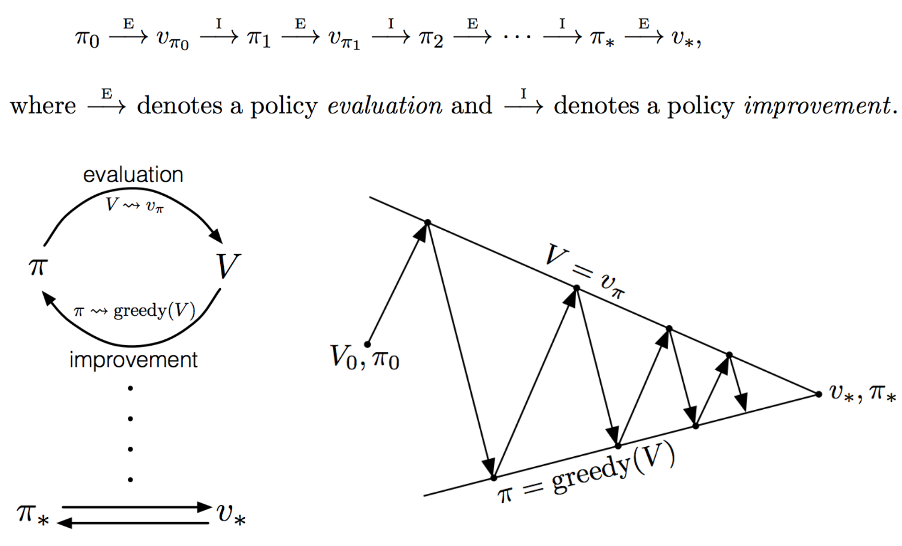
\includegraphics[width=0.9\columnwidth]{images/policy-iteration.png}
    \caption{Illustration of policy iteration}
    \label{fig:policy-iteration}
\end{figure}

Briefly speaking, we initially take a random policy $\pi$, then compute a state-value function $v_{\pi}$ and use $v_{\pi}$ to compute $q_{\pi}$. After that, we select the new greedy policy $\pi'(s)$ from $q_{\pi}$:
$$\pi'(s)= \argmax_a q_{\pi}(s,a)$$

Each policy is guaranteed to be an improvement on the last unless the last policy was already optimal.


\begin{tcolorbox}[title={Policy Iteration (using iterative policy evaluation) for estimating $\pi \approx \pi_*$}]

  \textbf{1. Initialization:} $V(s) \in \mathbb{R}$ and $\pi(s) \in \mathcal{A}(s)$ arbitrarily for all $s \in \mathcal{S}$ \\

  \textbf{2. Policy Evaluation:}
  \begin{description}
      \item $\;\;\;$ \textbf{Loop:}
      \begin{description}
        \item $\;\;\;$ $\Delta \leftarrow 0$
        \item $\;\;\;$ \textbf{Loop for each $s \in \mathcal{S}$:}
        \begin{description}
          \item $\;\;\;$ $v \leftarrow V(s)$
          \item $\;\;\;$ $V(s) \leftarrow \sum_{s', r} p(s',r|s,\pi(s)) [r + \gamma V(s')]$
          \item $\;\;\;$ $\Delta \leftarrow \max (\Delta , | v - V(s) |)$
        \end{description}
      \end{description}
      \textbf{Until:} $\Delta < \theta$ (a small positive number determining the accuracy of estimation)
  \end{description}

  \textbf{3. Policy Improvement:}
  \begin{description}
      \item $\;\;\;$ $policy–stable \leftarrow true$
      \item $\;\;\;$ \textbf{For each $s \in \mathcal{S}$:}
      \begin{description}
        \item $\;\;\;$ $old–action \leftarrow \pi(s)$
        \item $\;\;\;$ $\pi(s) \leftarrow \argmax_a \sum_{s', r} p(s',r | s,a)[r + \gamma V(s')]$
        \item $\;\;\;$ If $old–action \neq \pi(s)$, then $policy–stable \leftarrow false$
      \end{description}
      \item $\;\;\;$ If $policy–stable$, then stop and return $V \approx v_*$ and $\pi \approx \pi_*$; else go to 2
  \end{description}
\end{tcolorbox}



\subsection{Generalized Policy Iteration (GPI)}\label{generalized-policy-iteration}

\textbf{What:} We use the term generalized policy iteration (GPI) to refer to the \uline{general idea of letting \textcolor{blue}{policy evaluation} and \textcolor{blue}{policy improvement} processes interact}, independent of the granularity and other details of the two processes.

\textbf{Why:} Almost all reinforcement learning methods are well described as GPI.


\subsection{Value Iteration}\label{value-iteration}

\textbf{What:} a special case of generalized policy iteration.

\textbf{Why:} It allows us to \uline{\textbf{combine} \textcolor{blue}{policy evaluation} and \textcolor{blue}{policy improvement} into a single update}.


\begin{tcolorbox}[title={Value Iteration, for estimating  $\pi \approx \pi_*$}]

  \textbf{Algorithm parameters:}
  \begin{itemize}
    \item $\theta > 0 \leftarrow$ small threshold determining accuracy of estimation
  \end{itemize}

  \textbf{Initialize:}
  \begin{itemize}
    \item $V(s)$, for all $s \in \mathcal{S}^+$ arbitrarily
    \item $V(terminal) = 0$
  \end{itemize}


  \textbf{Loop:}
  \begin{description}
      \item $\;\;\;$ $\Delta \leftarrow 0$
      \item $\;\;\;$ \textbf{Loop for each $s \in \mathcal{S}$:}
      \begin{description}
        \item $\;\;\;$ $v \leftarrow V(s)$
        \item $\;\;\;$ $V(s) \leftarrow \max_a \sum_{s', r} p(s',r|s,a) [r + \gamma V(s')]$
        \item $\;\;\;$ $\Delta \leftarrow \max (\Delta , | v - V(s) |)$
      \end{description}
  \end{description}
  \textbf{Until:} $\Delta < \theta$ (a small positive number) \\

  \textbf{Output:} a deterministic policy, $\pi \approx \pi_*$, such that:
  \begin{description}
      \item $\;\;\;$ $\pi(s) = \argmax_a \sum_{s',r} p(s',r|s,a)[r+\gamma V(s')]$
  \end{description}
\end{tcolorbox}


We do not run policy evaluation to completion. We perform just one sweep over all the states. After that, we greedify again. We can write this as an update rule $V(s) \leftarrow \max_a \sum_{s', r} p(s',r|s,a) [r + \gamma V(s')]$ which applies directly to the state-value function. The \uline{update does not reference any specific policy, hence the name \textbf{value iteration}}.

\begin{itemize}
  \item \textcolor{Orange}{Instead of updating the value according to a fixed falsey}, \textcolor{blue}{we update using the action that maximizes the current value estimate}.
\end{itemize}



\subsection{Asynchronous Dynamic Programming}\label{asynchronous-dynamic-programming}

\textbf{What:} a special case of generalized policy iteration.

Asynchronous dynamic programming methods give us freedom to update states in any order, they do not perform systematic sweeps.

Asynchronous algorithms can propagate value information quickly through \textbf{selective updates}. This \uline{can sometimes be more efficient than a systematic sweep}.



\subsection{Efficiency of Dynamic Programming}\label{efficiency-of-dynamic-programming}

The \uline{\textbf{key insight of dynamic programming} is that we do not have to treat the evaluation of each state as a separate problem. We can use the other value estimates we have already worked so hard to compute}.

The process of \uline{using the value estimates of successor states to improve our current value estimate is known as \textbf{bootstrapping}}. This \textcolor{Green}{can be much more efficient than (e.g. a Monte Carlo) method that estimates each value independently}.

\begin{figure}[H]
  \centering  % Remember to centre the figure
    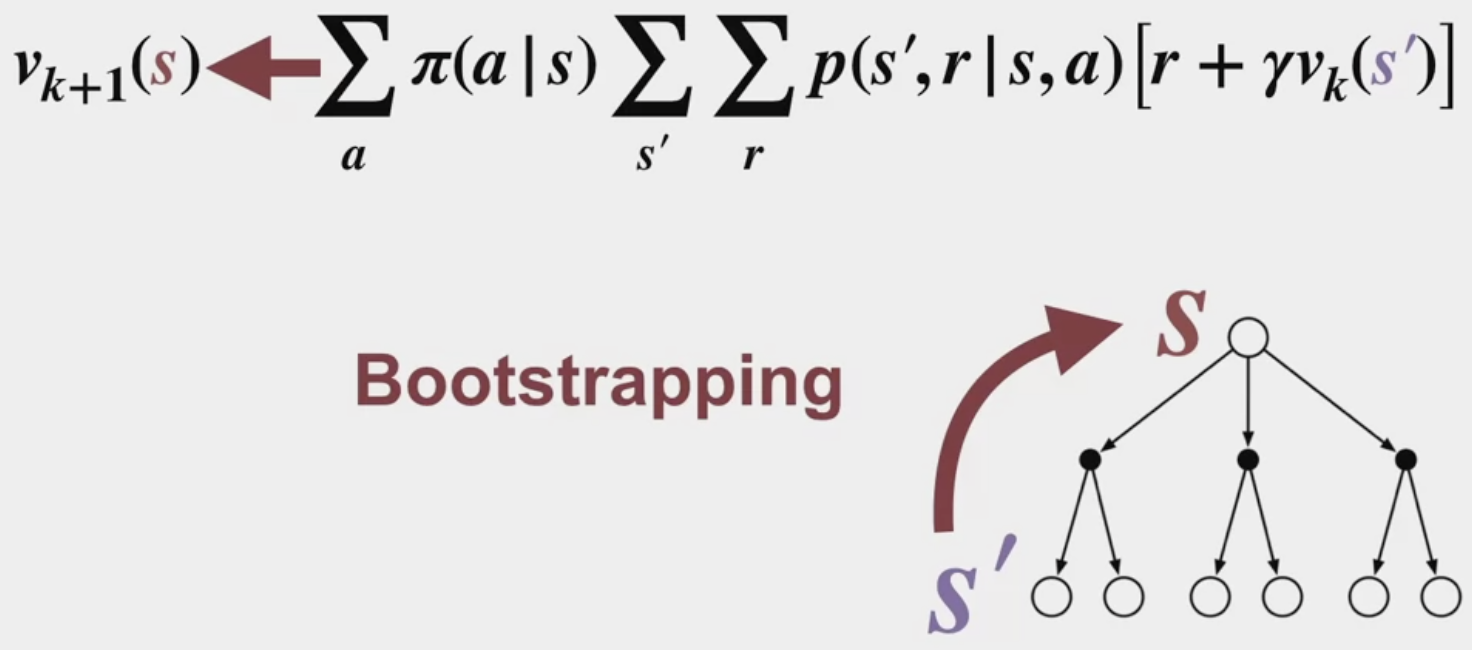
\includegraphics[width=0.8\columnwidth]{images/bootstrapping.png}
    \caption{Illustration of bootstrapping in Dynamic Programming}
    \label{fig:bootstrapping}
\end{figure}























% =============== CHAPTER 5 - Monte Carlo Methods ===============



\section{Monte Carlo Methods}\label{monte-carlo-methods}

\begin{tcolorbox}[colback=yellow!5,colframe=yellow!75!black,title=NOTE]
  To ensure that well-defined returns are available, here we define Monte
  Carlo methods only for \textbf{\colorbox{Yellow}{episodic tasks}}.
  \begin{itemize}
    \item That is, we assume experience is divided into episodes, and that all episodes eventually terminate no matter what actions are selected.
    \item Only on the completion of an episode are value estimates and policies changed.
  \end{itemize}
\end{tcolorbox}

\textbf{What:} sample-based methods for solving reinforcement learning problem.
\begin{itemize}
  \item \textbf{estimating} value functions \(\rightarrow\) \textbf{discovering}
  optimal policies.
\end{itemize}

\textbf{How:} based on \textbf{averaging} \uline{sample returns} \textbf{for
each} \uline{state--action pair}.

\textbf{Pros and cons:}
\begin{itemize}
  \item \textbf{+} Don't require a model (direct access to the environment dynamics) $\rightarrow$ Monte Carlo methods learn directly from interaction.
  \item \textbf{+} Conceptually simple
  \item \textbf{-} Not well suited for step-by-step incremental computation
\end{itemize}

\textbf{Base:}

\begin{itemize}
\item
  Unlike previously, we \textbf{don't assume complete knowledge of the
  environment}.

  \begin{itemize}
  \item
    Unknown transaction dynamics (T) and reward function (r)
  \end{itemize}
\item
  Require only \emph{experience} --- \textbf{sample} sequences of
  \textbf{states, actions, and rewards} from actual or simulated
  interaction with an environment.
\item
  There are \textbf{multiple states}, \emph{each acting like a different
  bandit problem} (like an associative-search or contextual bandit) and
  the different bandit problems are interrelated.
\end{itemize}

\textbf{Terms:}

\begin{itemize}
\item
  The term \textbf{``Monte Carlo''} is often used more broadly for any
  estimation method whose operation involves a significant random
  component.

  \begin{itemize}
  \item
    \textbf{HERE:} Here we use it specifically for methods based on
    averaging complete returns.
  \end{itemize}
\end{itemize}






\subsection{Monte Carlo Policy Evaluation (Prediction)}\label{monte-carlo-prediction}

\textbf{What:} \uline{\textbf{\textcolor{blue}{Monte Carlo methods}} for \textbf{Policy Evaluation}} (estimating value function $v_\pi$ for a specific policy $\pi$).


\textbf{Implications of MC learning:}

\begin{itemize}
  \item \textbf{learns directly from experience} $\rightarrow$ \textcolor{Green}{no need to keep a large model of the environment}.
  \item can \textbf{estimate the value of an individual state independently of the values of any other states}.
  \item \textbf{computation needed to update the value of each state} along the way \textcolor{Green}{doesn't depend in any way on the size of the MDP}.
  \begin{itemize}
    \item Rather, it \textcolor{Red}{depends on the length of the episode}.
  \end{itemize}
\end{itemize}



The \textbf{first-visit MC method} (focus of this chapter) estimates
\(v_\pi(s)\) as the average of the returns following first visits to s,
whereas the \textbf{every-visit MC method} averages the returns
following all visits to s.



\begin{tcolorbox}[title={First-visit MC prediction, for estimating $V \approx v_\pi$}]

  \textbf{Input:} a policy $\pi$ to be evaluated

  \textbf{Initialize:}
  \begin{itemize}
    \item $V(s) \in \mathbb{R}$, for all $s \in \mathcal{S}$ arbitrarily
    \item $Returns(s) \leftarrow$ an empty list, for all $s \in \mathcal{S}$
  \end{itemize}

  \textbf{Loop forever (for each episode):}
  \begin{description}
      \item $\;\;\;$ Generate an episode following $\pi$
      \item $\;\;\;$ $G \leftarrow 0$
      \item $\;\;\;$ \textbf{Loop for each step of episode, $t=T-1,T-2,...,0$:}
      \begin{description}
        \item $\;\;\;$ $G \leftarrow \gamma G + R_{t+1}$
        \item $\;\;\;$ \textbf{Unless $S_t$ appears in $S_0, S_1, ..., S_{t-1}:$}
        \begin{description}
          \item $\;\;\;$ Append $G$ to $Returns(S_t)$
          \item $\;\;\;$ $V(S_t) \leftarrow average(Returns(S_t))$
        \end{description}
      \end{description}
  \end{description}
\end{tcolorbox}

\begin{itemize}
  \item We can repeat the whole process over many episodes (loop forever) and \uline{eventually learn a good estimate for the value function}.
  \item \textbf{We can avoid keeping all the sampled returns in a list:} We can incrementally update the sample average estimated using the formula:
  \begin{gather*}
    Q_{n+1} = Q_n + \frac{1}{n}[R_n - Q_n] \\
    NewEstimate = OldEstimate + StepSize[Target - OldEstimate]
  \end{gather*}
\end{itemize}









\subsection{Monte Carlo Estimation of Action Values}\label{monte-carlo-estimation-of-action-values}


\textbf{What:} Using \uline{\textbf{\textcolor{blue}{Monte Carlo methods}} to learn \textbf{Action-Value functions $q_\pi$}} (instead of state-values).

\begin{itemize}
  \item Recall that we \textbf{learned state-values by} \uline{averaging sample returns from that state}.
  \item Similarny we \textbf{learn action-values by} \uline{averaging sample returns from that state, action pair}.
\end{itemize}


\textbf{Why:} Action values are useful for learning a policy. They allow us to \uline{compare different actions in the same state}. Then, we can switch to a better action if one is available.







\subsection{Monte Carlo Control}\label{monte-carlo-control}

\textbf{What:} Using \uline{\textbf{\textcolor{blue}{Monte Carlo methods}} to \textbf{approximate optimal policies}}. Namely Monte Carlo methods to implement a Generalized Policy Iteration (GPI) algorithm (\textcolor{blue}{policy evaluation} and \textcolor{blue}{policy improvement} processes interact).

\textbf{How:}

\begin{itemize}
  \item For the \textcolor{blue}{policy improvement step}, we can make the policy \uline{greedy with respect to the agent's current action value estimates}.
  \item For the \textcolor{blue}{policy evaluation step}, we will use a \uline{Monte Carlo method to estimate the action values}.
  \item For Monte Carlo policy iteration it is natural to \textbf{alternate between} \textcolor{blue}{evaluation} and \textcolor{blue}{improvement} on an \uline{episode-by-episode basis}.
  \begin{itemize}
    \item \textbf{After each episode},
    \begin{enumerate}
      \item the \textbf{observed returns} are \uline{used for \textcolor{blue}{policy evaluation}}, and
      \item then the \uline{\textcolor{blue}{policy is improved} at all the states visited in the episode}.
    \end{enumerate}
  \end{itemize}
\end{itemize}


\begin{figure}[H]
  \centering  % Remember to centre the figure
    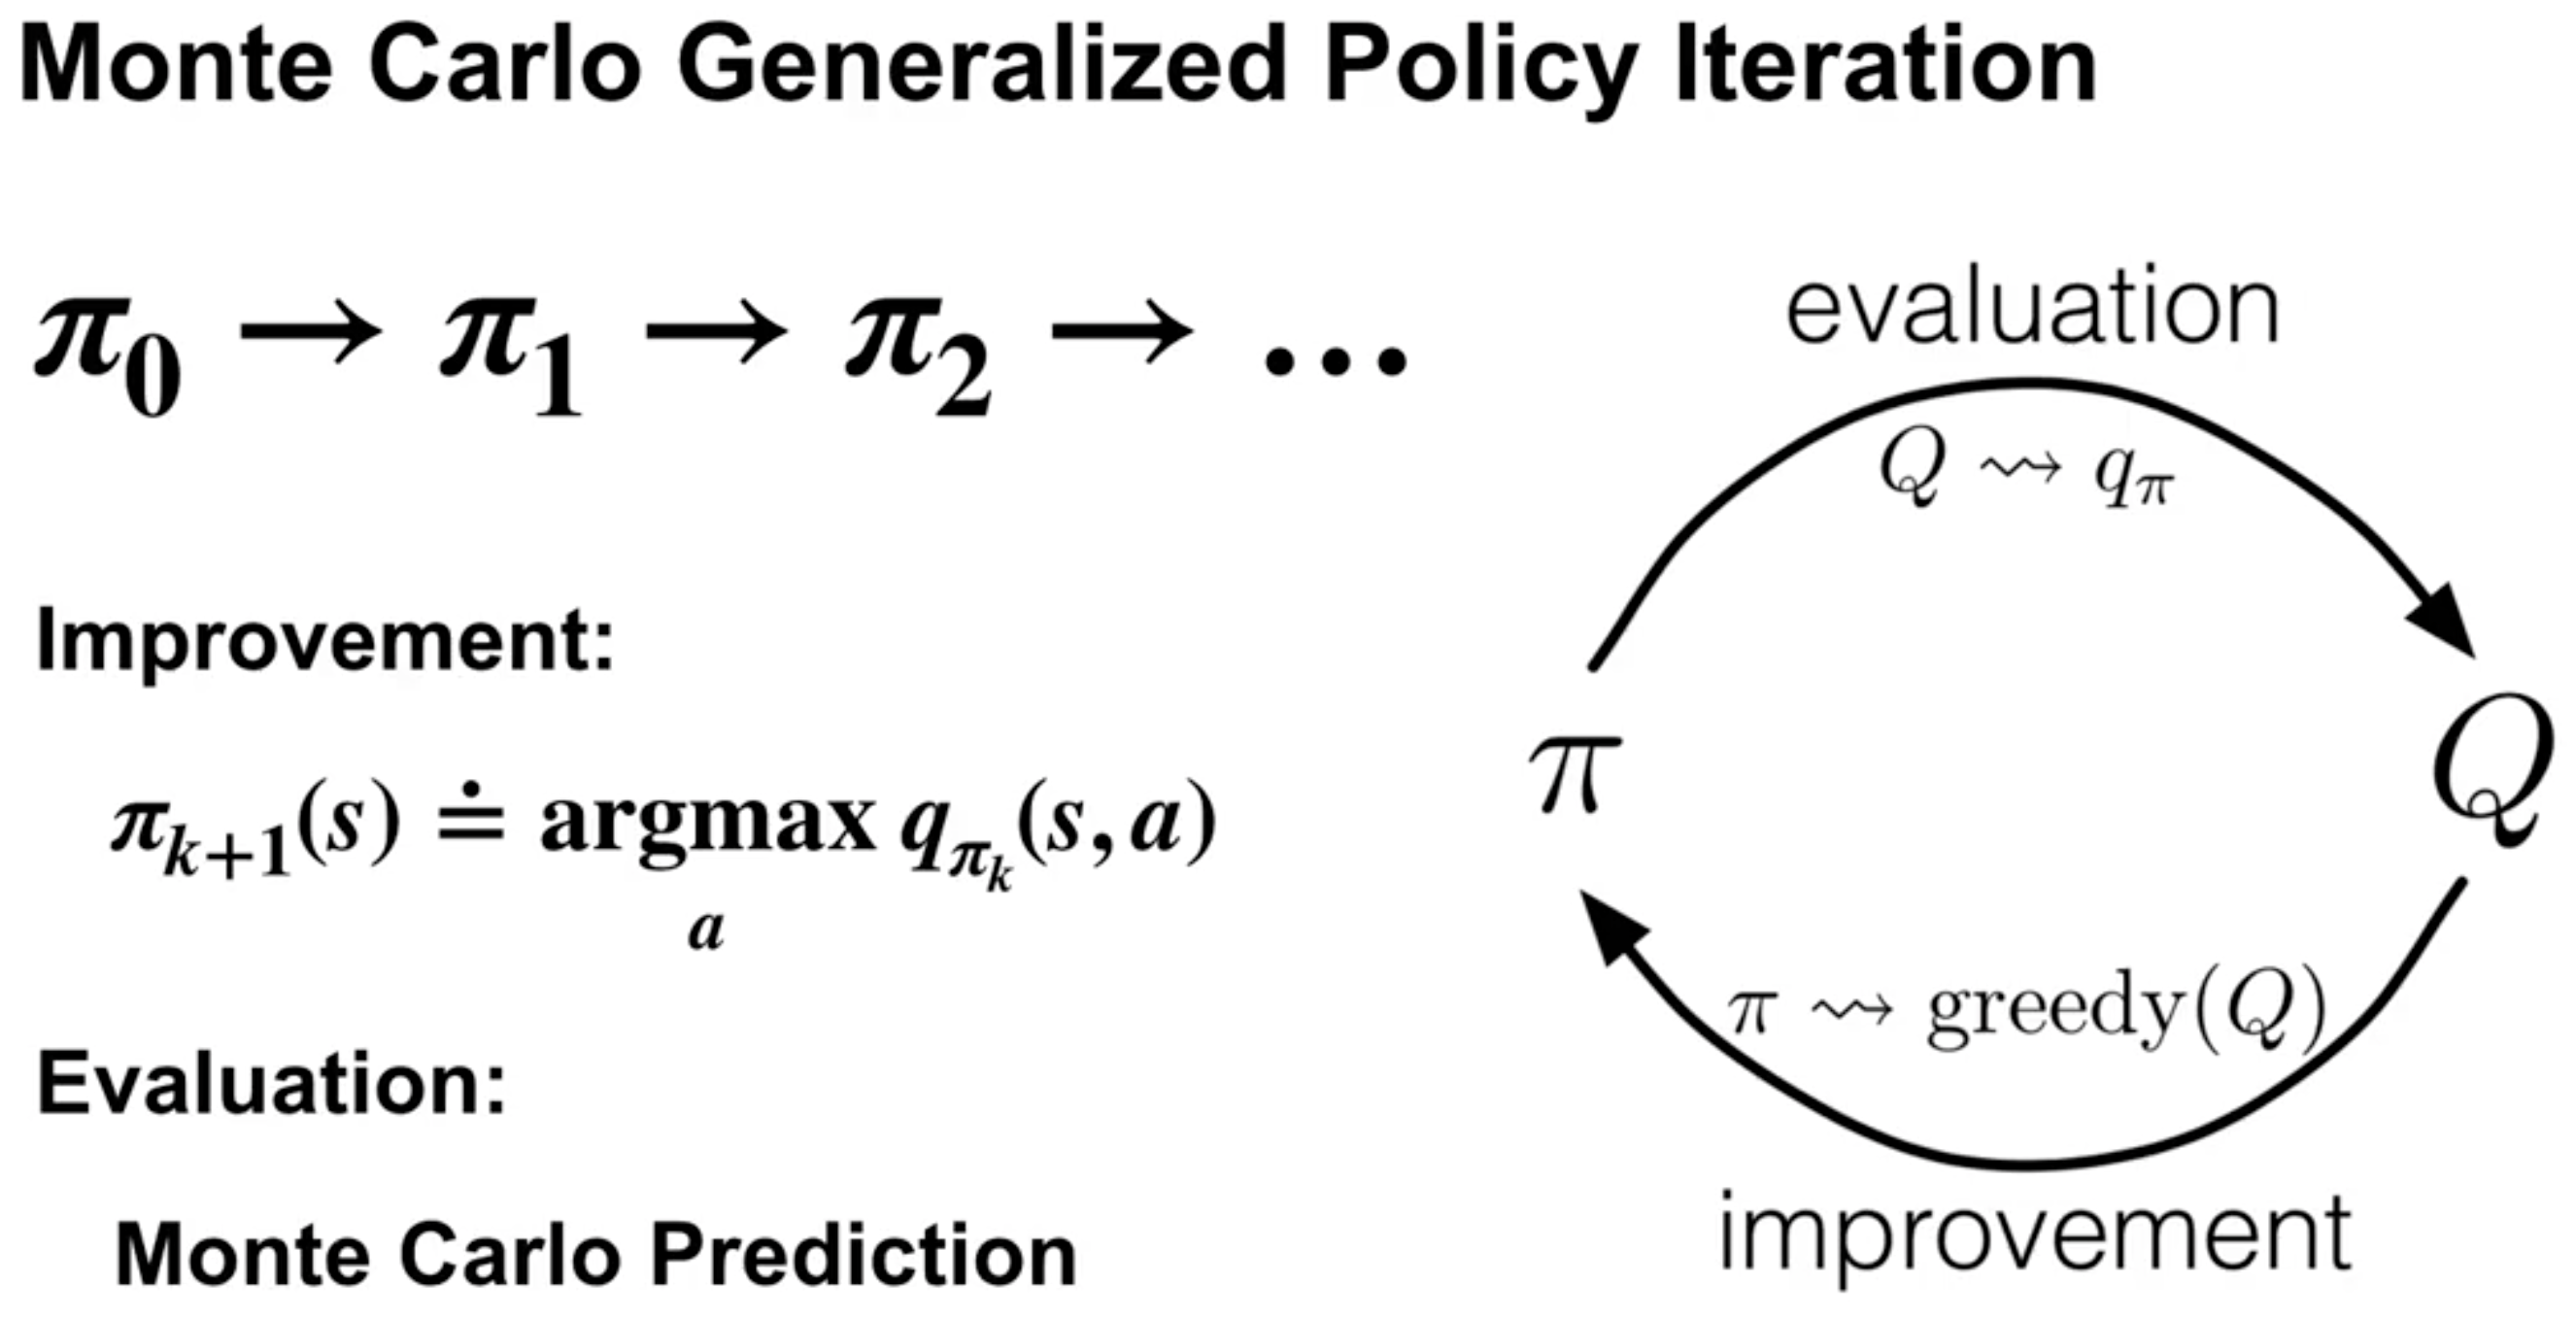
\includegraphics[width=0.8\columnwidth]{images/monte-carlo-policy-iteration.png}
    \caption{Process of Monte Carlo General Policy Iteration.}
    \label{fig:monte-carlo-policy-iteration}
\end{figure}

 A complete simple algorithm along these lines, which we call Monte Carlo ES, for Monte Carlo with Exploring Starts, is given in pseudocode below.



\begin{tcolorbox}[title={Monte Carlo ES (Exploring Starts), for estimating $\pi \approx \pi_*$}]

\textbf{Initialize:}
\begin{itemize}
 \item $\pi(s) \in \mathcal{A}(s)$, for all $s \in \mathcal{S}$ arbitrarily
 \item $Q(s,a) \in \mathbb{R}$ for all $s \in \mathcal{S}, a \in \mathcal{A}(s)$ arbitrarily
\end{itemize}

\textbf{Loop forever (for each episode):}
\begin{description}
   \item $\;\;\;$ Choose $S_0 \in \mathcal{S}, A_0 \in \mathcal{A}(\mathcal{S}_0)$ randomly such that all pairs have probability $> 0$
   \item $\;\;\;$ Generate an episode from $S_0$, $A_0$, following $\pi$
   \item $\;\;\;$ $G \leftarrow 0$
   \item $\;\;\;$ \textbf{Loop for each step of episode, $t=T-1,T-2,...,0$:}
   \begin{description}
     \item $\;\;\;$ $G \leftarrow \gamma G + R_{t+1}$
     \item $\;\;\;$ \textbf{Unless $S_t, A_t$ appears in $S_0, A_0, S_1, A_1, ..., S_{t-1}, A_{t-1}:$}
     \begin{description}
       \item $\;\;\;$ Append $G$ to $Returns(S_t, A_t)$
       \item $\;\;\;$ $Q(S_t, A_t) \leftarrow average(Returns(S_t, A_t))$
       \item $\;\;\;$ $\pi(S_t) \leftarrow \argmax_a Q(S_t, a)$
     \end{description}
   \end{description}
\end{description}
\end{tcolorbox}

\begin{itemize}
  \item \textbf{Exploring start:} For policy evaluation to work for action values, we must \uline{assure continual exploration}. One way to do this is by specifying that the \uline{episodes start in a state–action pair, and that every pair has a nonzero probability of being selected as the start}. This guarantees that all state–action pairs will be visited an infinite number of times in the limit of an infinite number of episodes.
\end{itemize}








\subsection{Monte Carlo Control without Exploring Starts}\label{monte-carlo-control-without-exploring-starts}

\textbf{What:} Alternative ways (to Exploring Starts) for performing exploration. Here we use $\epsilon$-Soft policies.

\textbf{Why:} It can be difficult to randomly sample an initial State action pair.

\begin{itemize}
  \item e.g. For example, how would you randomly sample the initial State action pair for a self-driving car? How could we ensure the agent can start in all possible States? We would need to put the car in many different configurations in the middle of a busy freeway. This would be dangerous and impractical.
\end{itemize}



\textbf{\textcolor{blue}{$\epsilon$-Soft policies}:} take each action with probability at least Epsilon over the number of actions ($\epsilon/|\mathcal{A}|$).

\begin{figure}[H]
  \centering  % Remember to centre the figure
    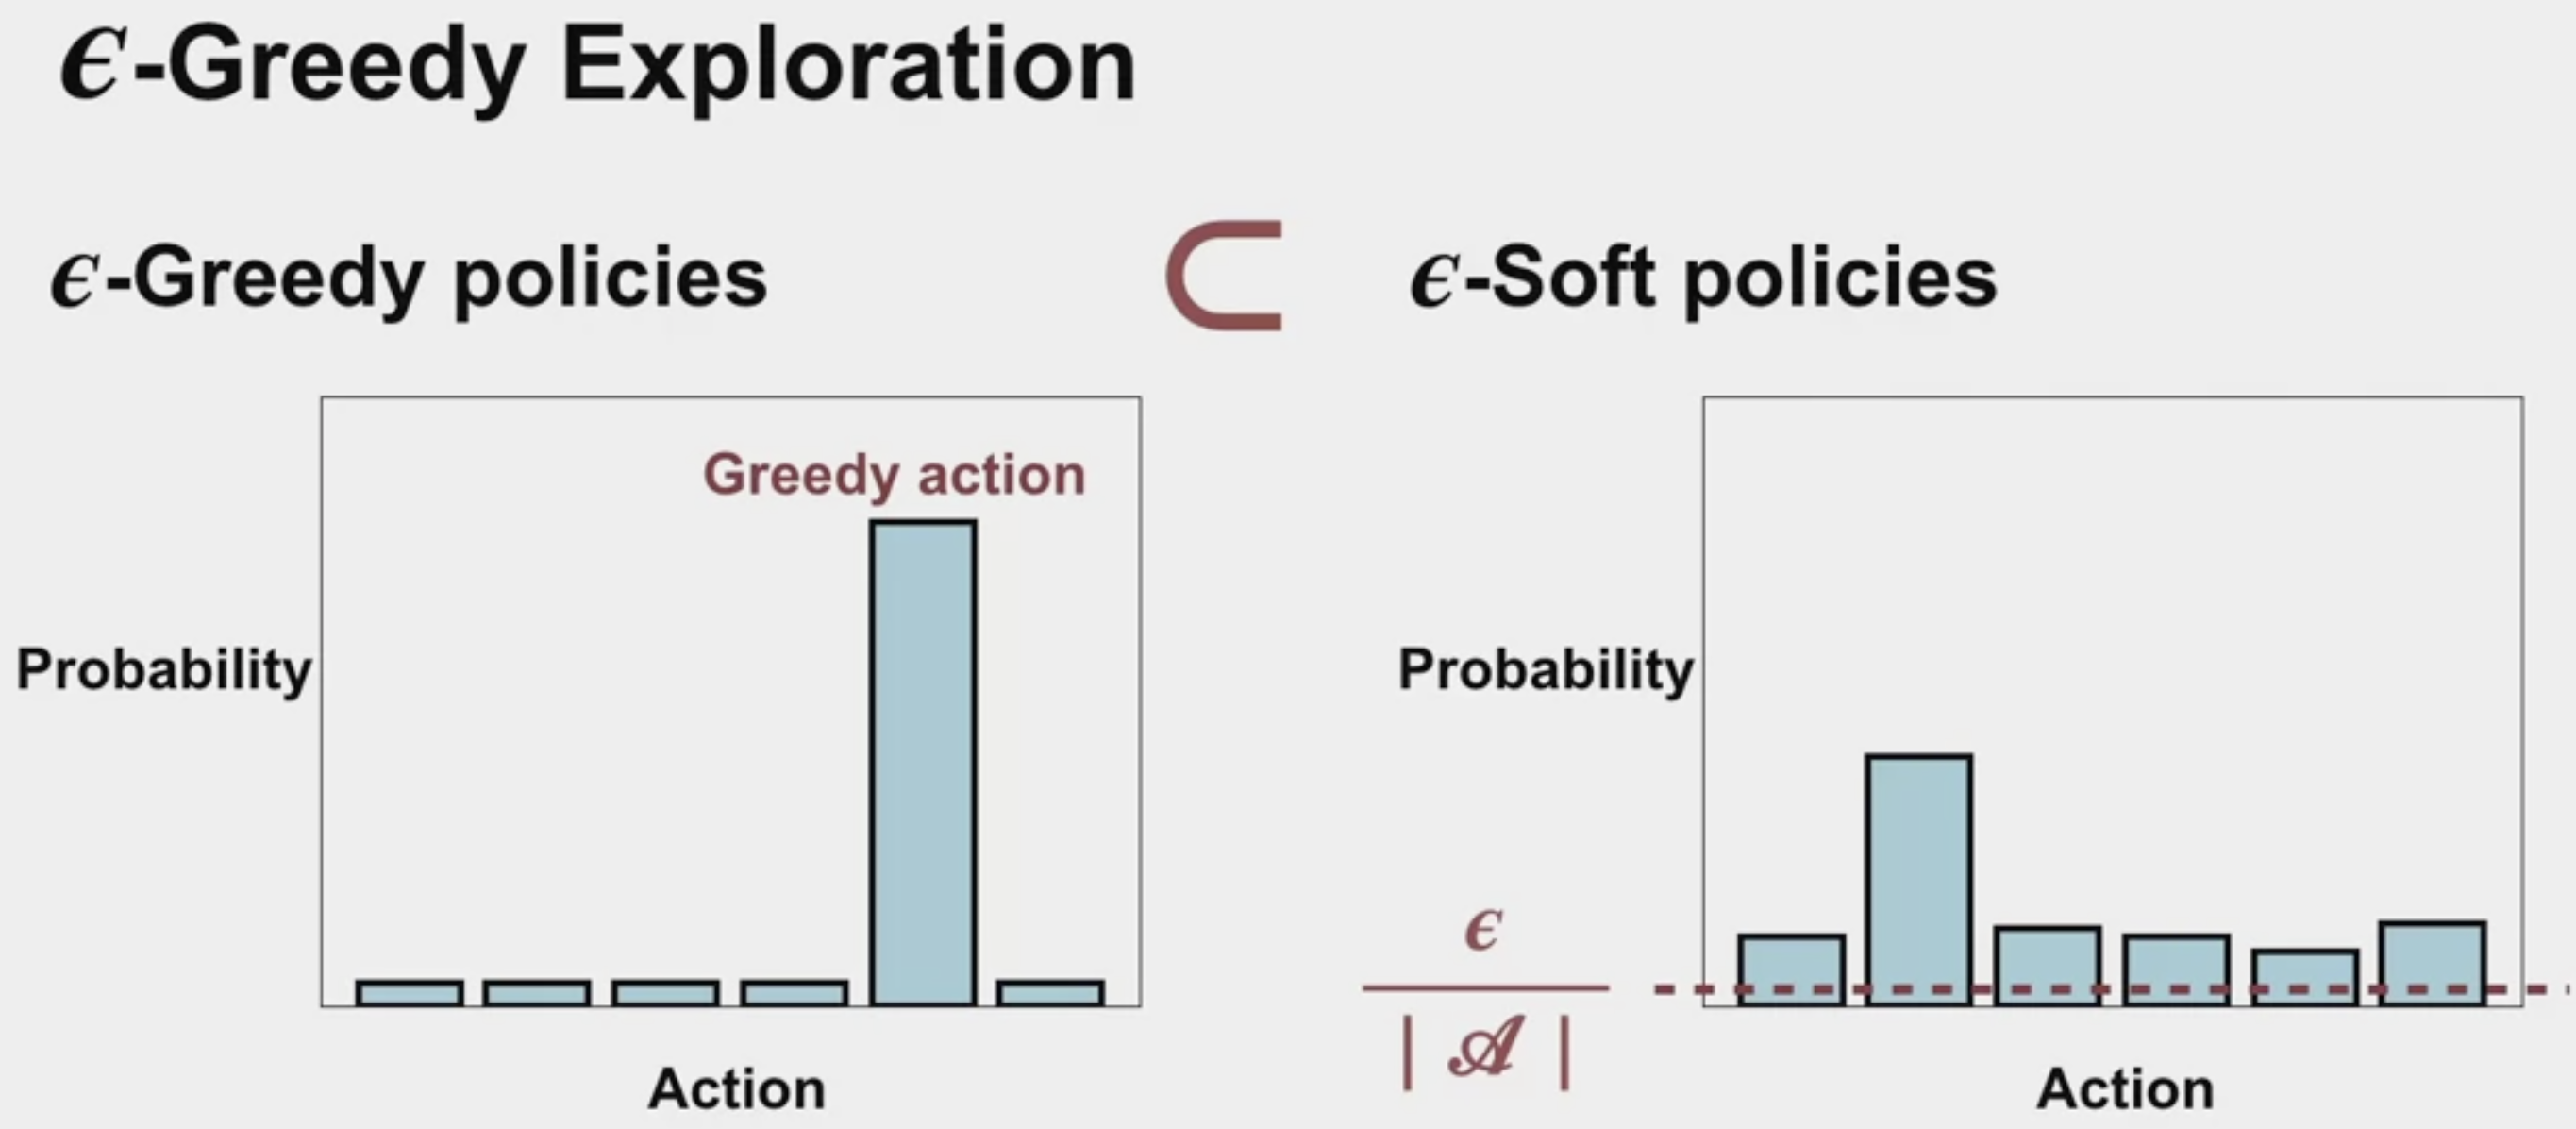
\includegraphics[width=1.0\columnwidth]{images/epsilon-soft-policies.png}
    \caption{$\epsilon$-greedy policies are a subset of $\epsilon$-soft policies}
    \label{fig:monte-carlo-policy-iteration}
\end{figure}

However, if our policy always gives at least Epsilon probability to each action, it's \textcolor{Red}{impossible to converge to a deterministic optimal policy}
$$
\pi_* > Optimal\;\epsilon–soft
$$


We will later discuss how \textcolor{Green}{we can learn the optimal policy using a different method called \textbf{Q-learning}}.


\begin{tcolorbox}[title={On-policy first-visit MC control (for $\epsilon$-soft policies), estimates $\pi \approx \pi_*$}]

\textbf{Algorithm parameter:} small $\epsilon$ > 0

\textbf{Initialize:}
\begin{itemize}
 \item $\pi(s) \leftarrow$ an arbitrary $\epsilon$-soft policy
 \item $Q(s,a) \in \mathbb{R}$ for all $s \in \mathcal{S}, a \in \mathcal{A}(s)$ arbitrarily
 \item $Returns(s,a) \leftarrow$ an empty list, for all $s \in \mathcal{S}, a \in \mathcal{A}(s)$
\end{itemize}

\textbf{Repeat forever (for each episode):}
\begin{description}
   \item $\;\;\;$ Generate an episode from $S_0$, $A_0$, following $\pi$:
   \item $\;\;\;$ $G \leftarrow 0$
   \item $\;\;\;$ \textbf{Loop for each step of episode, $t=T-1,T-2,...,0$:}
   \begin{description}
     \item $\;\;\;$ $G \leftarrow \gamma G + R_{t+1}$
     \item $\;\;\;$ \textbf{Unless $S_t, A_t$ appears in $S_0, A_0, S_1, A_1, ..., S_{t-1}, A_{t-1}:$}
     \begin{description}
       \item $\;\;\;$ Append $G$ to $Returns(S_t, A_t)$
       \item $\;\;\;$ $Q(S_t, A_t) \leftarrow average(Returns(S_t, A_t))$
       \item $\;\;\;$ $A^* \leftarrow \argmax_a Q(S_t,a)$     (with ties broken arbitrarily)
       \item $\;\;\;$ For all $a \in \mathcal{A}(S_t)$
       $$
       \pi(a|S_t)=
        \begin{cases}
           1-\epsilon + \epsilon / |\mathcal{A}(S_t)| & \text{if } a = A^* \\
          \epsilon / |\mathcal{A}(S_t)| & \text{if } a \neq A^*
        \end{cases}
       $$
     \end{description}
   \end{description}
\end{description}
\end{tcolorbox}






\subsection{Off-policy Prediction via Importance Sampling}\label{off-policy-prediction-via-importance-sampling}

\textbf{What:} Importance sampling allowing us to do Off-Policy learning. More precisely, we use the important sampling ratios to correct the returns generated by a behavior policy and we modified the on-policy Monte Carlo prediction algorithm for off-policy learning.

\textbf{Why:} Off-Policy learning allows us to learn optimal policy from suboptimal behaviour. This way we can \textcolor{Green}{learn an optimal policy but still maintain exploration}.

\textbf{On-Policy vs. Off-Policy:}
\begin{itemize}
  \item \textbf{\textcolor{Blue}{On-Policy}:} \textcolor{blue}{improve} and \textcolor{blue}{evaluate} the \uline{policy being used to select actions}.
  \item \textbf{\textcolor{Blue}{Off-Policy}:} \textcolor{blue}{improve} and \textcolor{blue}{evaluate} a \uline{different policy (\textcolor{Blue}{behavio policy $b(s|a)$}) from the one used to select actions (\textcolor{Blue}{target policy $\pi(s|a)$})}.
  \begin{itemize}
    \item \textcolor{Blue}{behavio policy $b(s|a)$} is generally an \uline{exploratory policy}
    \item One key rule of off policy learning is that the behavior policy must cover the target policy
    $$
    \text{If } \pi(a|s) > 0 \text{ then also } b(a|s) > 0
    $$
  \end{itemize}
  \item Learning \textcolor{Blue}{on-policy} or \textcolor{Blue}{off-policy} \textcolor{Orange}{may perform differently in control depending on the task}.
\end{itemize}


\textbf{Importance Sampling:} A way of \uline{estimating the expected value of a distribution using samples from a different distribution}.
\begin{itemize}
  \item Derivation of Importance Sampling – Consider:
  \begin{itemize}
    \item Random variable $x$ is being sampled from a probability distribution $b$
    $$
    \text{Sample: } x \sim b
    $$
    \item We want to estimate the expected value of $x$, but with respect to the target distribution $\pi$.
    $$
    \text{Estimate: } \mathbb{E}_\pi[X]
    $$

    \item \textcolor{Red}{Because $x$ is drawn from $b$, we cannot simply use the sample average to compute the expectation under $\pi$.}

    \item We can use importance sampling to correct the expectation:
      \begin{align*}
      \mathbb{E}_\pi[X] &=
      \sum_{x \in X} x \frac{\pi(x)}{b(x)} b(x) \\
      &= \sum_{x \in X} x \underbrace{\rho(x)}_\text{importance sampling ratio}b(x) \\
      &= \mathbb{E}_b [X\rho(x)] \\
      \end{align*}
    \item We can then use importance sampling to \textbf{estimate the expectation from data:} We just need to compute a \uline{weighted sample average with the importance sampling ratio as the weightings}:
      \begin{align*}
      \mathbb{E}_b [X\rho(x)] &=
      \sum_{x \in X} x \rho(x) b(x) \\
      &\approx \frac{1}{n} \sum_{i=1}^n x_i \rho(x_i)
      \end{align*}
    \item \textcolor{Green}{We can now estimate the expected value of $x$ under distribution $\pi$ by using the sample average, the samples drawn from distribution $b$.}

    \begin{figure}[H]
      \centering  % Remember to centre the figure
        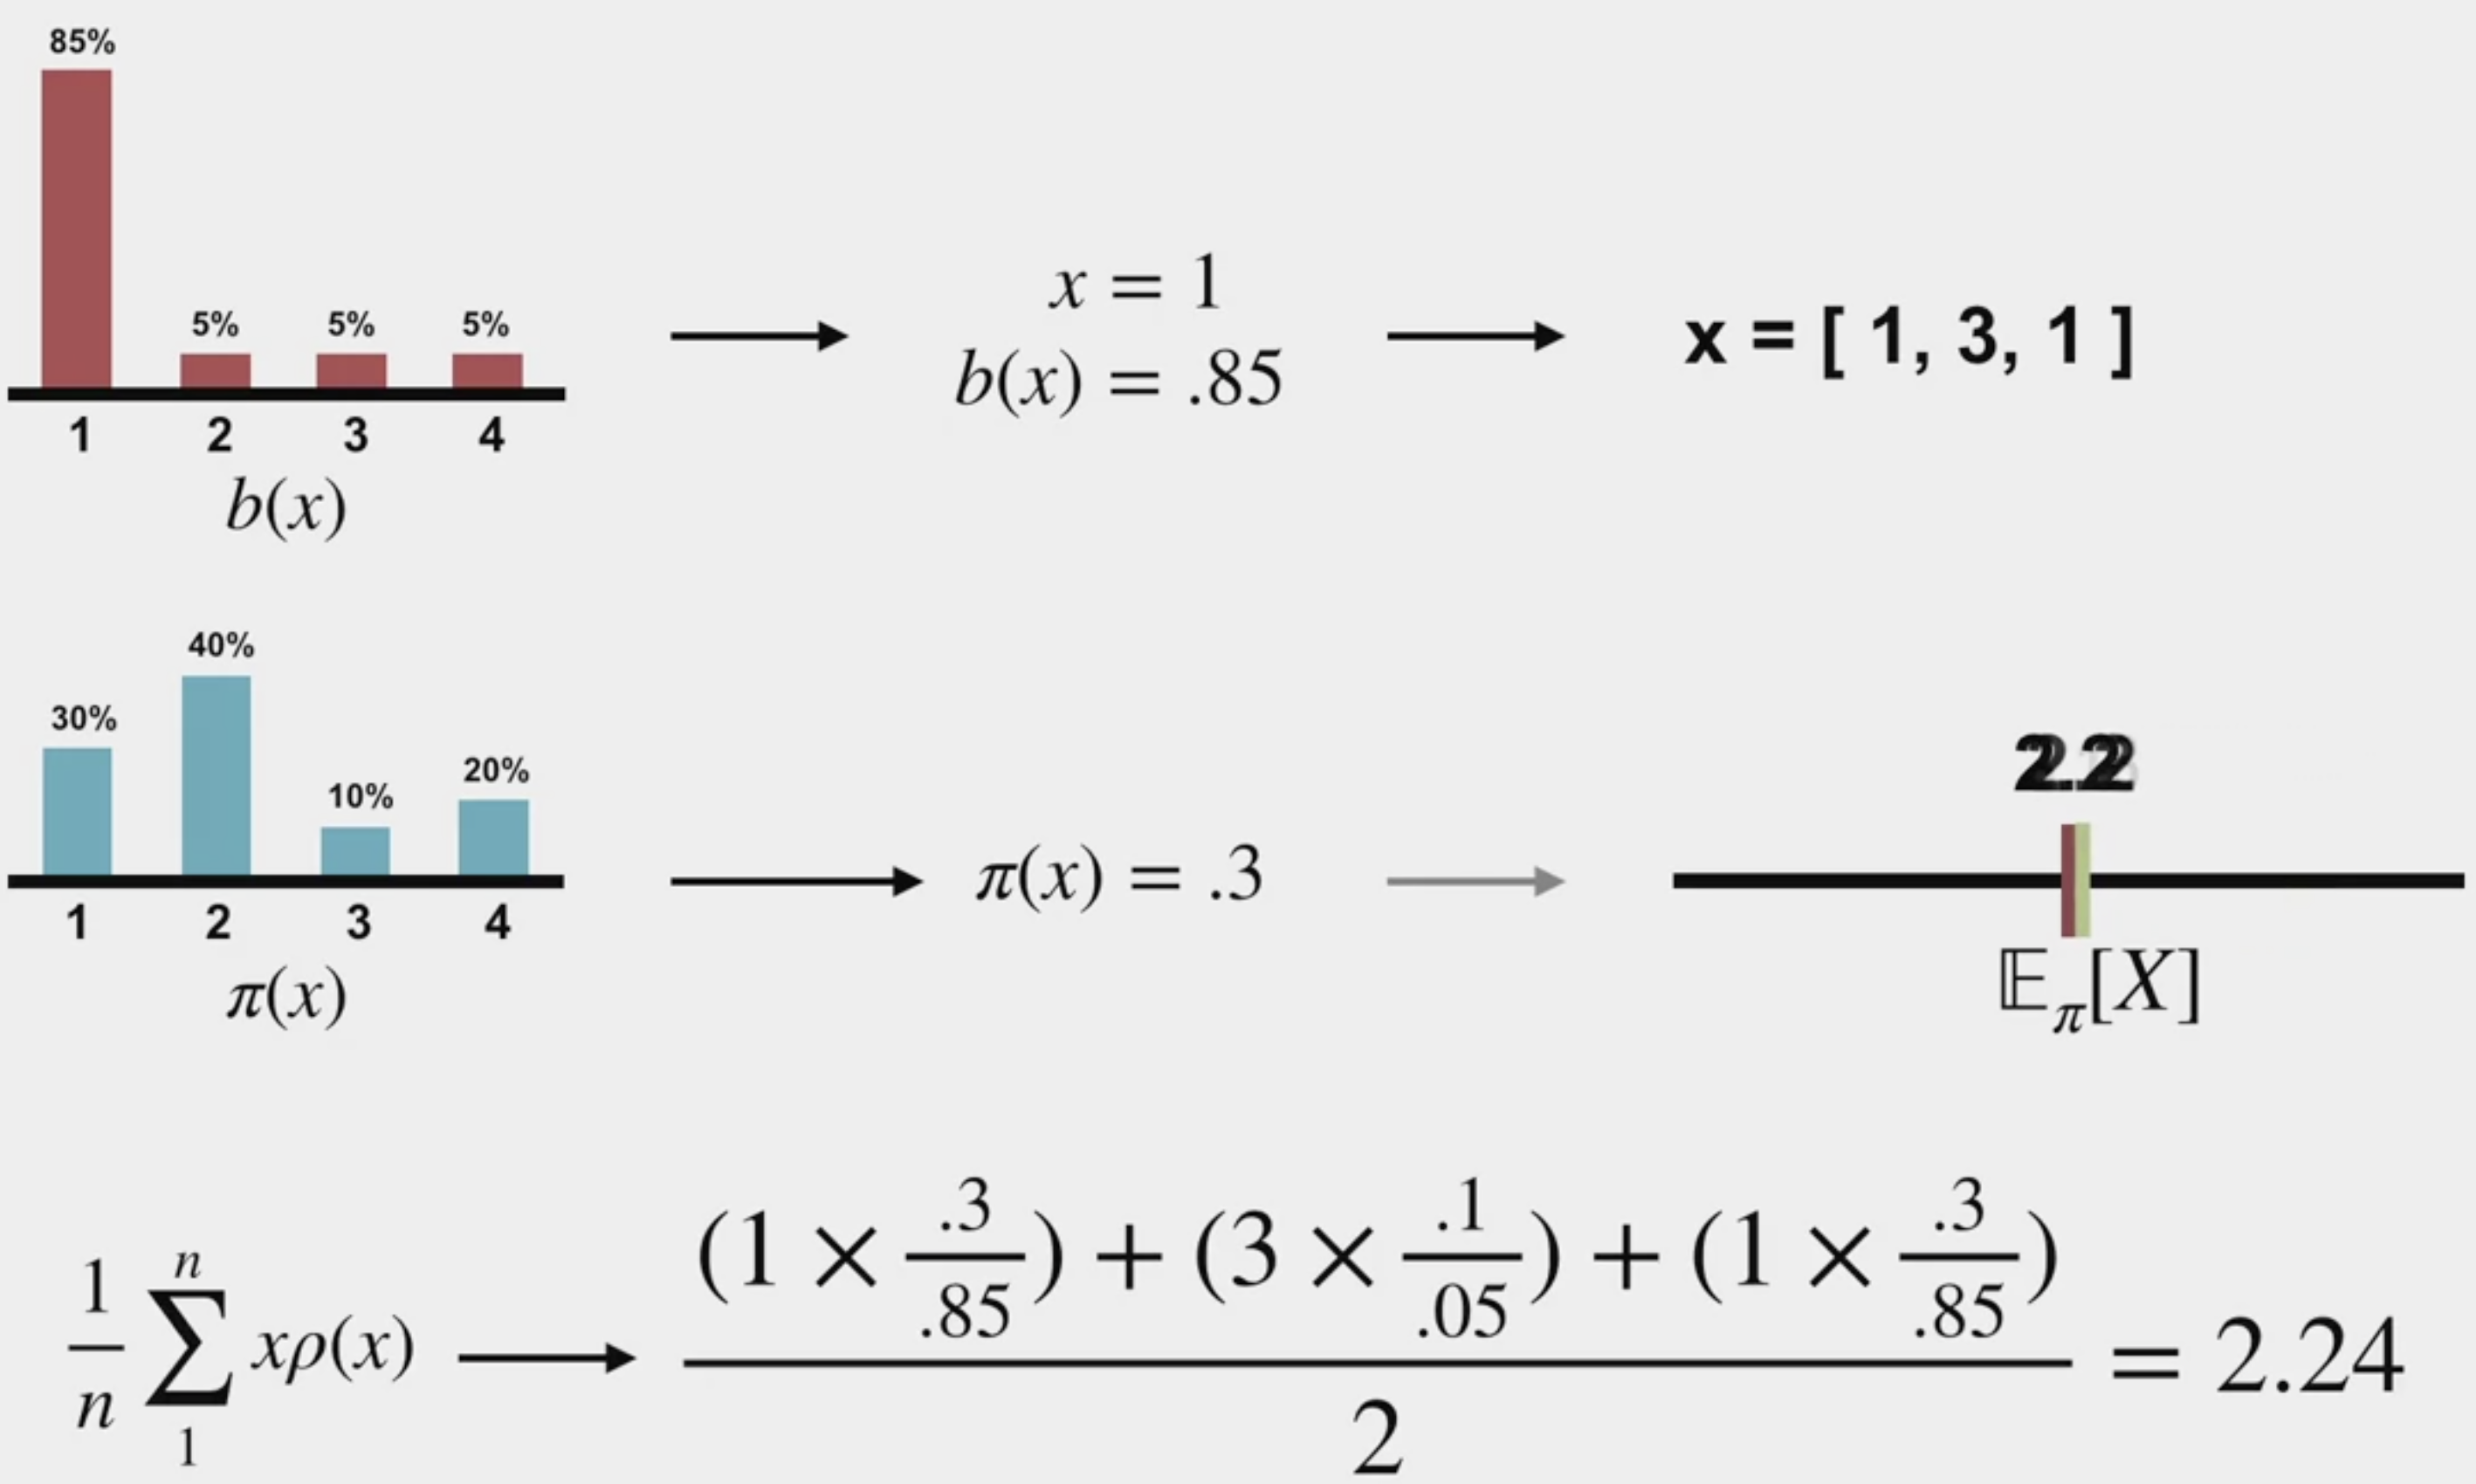
\includegraphics[width=0.7\columnwidth]{images/importance-sampling-eg.png}
        \caption{Example importance sampling (samples 1, 3 \& 1)}
        \label{fig:importance-sampling-eg}
    \end{figure}
    \begin{itemize}
      \item With samples just from $b$, we managed to get a pretty good estimate of the expectation under $\pi$.
    \end{itemize}
  \end{itemize}
\end{itemize}


\textbf{Off-policy Prediction via Importance Sampling:}
\begin{itemize}
  \item The expectation of the return under $\pi$, sampling from $b$:
  \begin{gather*}
  V_\pi(s) = \mathbb{E}_b [\rho G_t | S_t = s] \\ \\
  \textbf{Where:} \\
  \text{Rho: } \rho = \frac{\mathbb{P}(\text{trajectory under $\pi$})}{\mathbb{P}(\text{trajectory under $b$})} \\
  = \prod_{k=t}^{T-1} \frac{\pi(A_k | S_k)}{b(A_k | S_k)} \\ \\
  \textbf{Where:} \\
  \mathbb{P}(\text{trajectory under $b$}) = \prod_{k=t}^{T-1} b(A_k | S_k) p(S_{k+1} | S_k, A_k) \\
  \mathbb{P}(\text{trajectory under $\pi$}) = \prod_{k=t}^{T-1} \pi(A_k | S_k) p(S_{k+1} | S_k, A_k) \\
\end{gather*}
\end{itemize}




\textbf{Incremental Implementation:}

Monte Carlo prediction methods can be implemented incrementally, on an episode-by-episode basis, using average returns.


\begin{tcolorbox}[title={Off-policy MC prediction (policy evaluation) for estimating $Q \approx q_\pi$}]


\textbf{Input:} an arbitrary target policy $\pi$

\textbf{Initialize, for all $s \in \mathcal{S}, a \in \mathcal{A}(s)$:}
\begin{itemize}
 \item $Q(s,a) \in \mathbb{R}$ (arbitrarily)
 \item $C(s,a) \leftarrow 0$
\end{itemize}

\textbf{Loop forever (for each episode):}
\begin{description}
   \item $\;\;\;$ $b$ any policy with coverage of $\pi$
   \item $\;\;\;$ Generate an episode following $b$
   \item $\;\;\;$ $G \leftarrow 0$
   \item $\;\;\;$ $W \leftarrow 1$
   \item $\;\;\;$ \textbf{Loop for each step of episode, $t=T-1,T-2,...,0$, while $W \neq 0$:}
   \begin{description}
     \item $\;\;\;$ $G \leftarrow \gamma G + R_{t+1}$
     \item $\;\;\;$ $C(S_t,A_t) \leftarrow C(S_t,A_t) + W$
     \item $\;\;\;$ $Q(S_t,A_t) \leftarrow Q(S_t,A_t) + \frac{W}{C(S_t,A_t)} [G - Q(S_t,A_t)]$
     \item $\;\;\;$ $W \leftarrow W\frac{\pi(A_k | S_k)}{b(A_k | S_k)}$
   \end{description}
\end{description}
\end{tcolorbox}

\begin{itemize}
  \item $W:$ accumulated product of important sampling ratios on each time step of the episode.
  \item We compute Rho $\rho$ from $t$ to $T-1$ incrementally ($W = \rho_{t:T-1}$).
  $$
  W_{t+1} \leftarrow W_t \rho_t
  $$
  \begin{itemize}
    \item We can compute this recursively without having to store all past values of Rho.
  \end{itemize}
\end{itemize}













\subsection{Off-policy Monte Carlo Control}\label{off-policy-monte-carlo-control}


\begin{tcolorbox}[title={Off-policy MC control for estimating $\pi \approx \pi_*$}]

\textbf{Initialize, for all $s \in \mathcal{S}, a \in \mathcal{A}(s)$:}
\begin{itemize}
 \item $Q(s,a) \in \mathbb{R}$ (arbitrarily)
 \item $C(s,a) \leftarrow 0$
 \item $\pi(s) \leftarrow \argmax_a Q(s,a)$ (with ties broken consistently)
\end{itemize}

\textbf{Loop forever (for each episode):}
\begin{description}
   \item $\;\;\;$ $b$ any soft policy
   \item $\;\;\;$ Generate an episode using $b$
   \item $\;\;\;$ $G \leftarrow 0$
   \item $\;\;\;$ $W \leftarrow 1$
   \item $\;\;\;$ \textbf{Loop for each step of episode, $t=T-1,T-2,...,0$:}
   \begin{description}
     \item $\;\;\;$ $G \leftarrow \gamma G + R_{t+1}$
     \item $\;\;\;$ $C(S_t,A_t) \leftarrow C(S_t,A_t) + W$
     \item $\;\;\;$ $Q(S_t,A_t) \leftarrow Q(S_t,A_t) + \frac{W}{C(S_t,A_t)} [G - Q(S_t,A_t)]$
     \item $\;\;\;$ $\pi(S_t) \leftarrow \argmax_a Q(S_t,a)$ (with ties broken consistently)
     \item $\;\;\;$ If $A_t \neq \pi(S_t)$ then exit inner Loop (proceed to next episode)
     \item $\;\;\;$ $W \leftarrow W\frac{1}{b(A_t | S_t)}$
   \end{description}
\end{description}
\end{tcolorbox}















% =============== CHAPTER 6 - Temporal-Difference Learning ===============



\section{Temporal-Difference (TD) Learning}\label{temporal-difference-learning}


\begin{tcolorbox}[colback=green!5,colframe=green!75!black]
  One of the most fundamental concepts in reinforcement learning!
\end{tcolorbox}


\textbf{What:} class of \uline{model-free} reinforcement learning methods which learn by \uline{bootstrapping} from the current estimate of the value function. These methods are a \uline{combination of \textcolor{blue}{Monte Carlo (MC)} ideas and \textcolor{blue}{dynamic programming (DP)} ideas}.

\textbf{How:}
\begin{itemize}
  \item Like \textcolor{blue}{MC}, TD methods can \uline{learn directly from raw experience without a model of the environment’s dynamics}.
  \item Like \textcolor{blue}{DP}, TD methods \uline{update estimates based in part on other learned estimates, without waiting for a final outcome (they bootstrap)}.
\end{itemize}

For the control problem (finding an optimal policy), DP, TD, and MC methods \uline{all use some variation of \textbf{generalized policy iteration (GPI)}}. The differences in the methods are primarily differences in their approaches to the prediction problem.










\subsection{TD Prediction}\label{td-prediction}

\textbf{TD vs. MC}
\begin{itemize}
  \item \textbf{Both} \uline{use experience to solve the prediction problem}.
  \item \textbf{\textcolor{blue}{MC methods}} \uline{wait until the end of the episode to determine the increment to $V(S_t)$} (only then is $G_t$ known).
  \item \textbf{\textcolor{blue}{TD methods}} \uline{wait only until the next time step}. At time $t + 1$ they immediately form a target and make a useful update using the observed reward $R_{t+1}$ and the estimate $V (S_{t+1})$.
\end{itemize}


\textbf{We can use these recursive formula to incrementally update our estimated value:}

First recall:
\begin{itemize}
  \item \textbf{$G_t$ (recursively):}
  $$
  G_t \dot{=} R_{t+1} + \gamma G_{t+1}
  $$
  \item \textbf{$v_\pi(s)$ (recursively):}
    \begin{align*}
    v_\pi(s) &= \mathbb{E}_\pi[R_{t+1} + \gamma G_{t+1}|S_t=s] \\
    &= R_{t+1} + \gamma v_\pi(S_{t+1})
    \end{align*}
\end{itemize}

Incremental Monte Carlo update rule (Monte Carlo estimate without saving lists of returns):
$$V(S_t) \leftarrow V(S_t) + \alpha [G_t - V(S_t)]$$
\begin{itemize}
  \item We can replace $G_t$ with the \uline{reward + the estimate of the return in the next state} (so we \textcolor{Green}{don't have to wait until the end of the episode}, but we still have to wait to the next step):
  $$V(S_t) \leftarrow V(S_t) + \alpha \underbrace{[\underbrace{R_{t+1} + \gamma V(S_{t+1})}_\text{t target} - V(S_t)]}_\text{TD-error $\delta_t$}$$
  \item TD updates the value of one state towards its own estimate of the value in the next state. As the estimated value for the next state improves, so does our target.
  \begin{itemize}
    \item \textcolor{Orange}{In fact, we've done something like this before in dynamic programming. In DP, we update $V(S_t)$ toward the value of all possible next states. The primary difference is in DP, we use an expectation over all possible next states. We needed a model of the environment to compute this expectation, in TD we only need the next state. We can get that directly from the environment without a model.}
  \end{itemize}

  We can get the next state directly from the environment without a model, \textbf{1-Step TD}:
  \begin{itemize}
    \item Think of time $t+1$ as the current time step and time $t$ as the previous time step.
    \item Simply store the state from the previous time step in order to make our TD updates: $s_t \leftarrow s_{t+1}$
    \item Only then can we update the value of the previous state.
    \begin{figure}[H]
      \centering  % Remember to centre the figure
        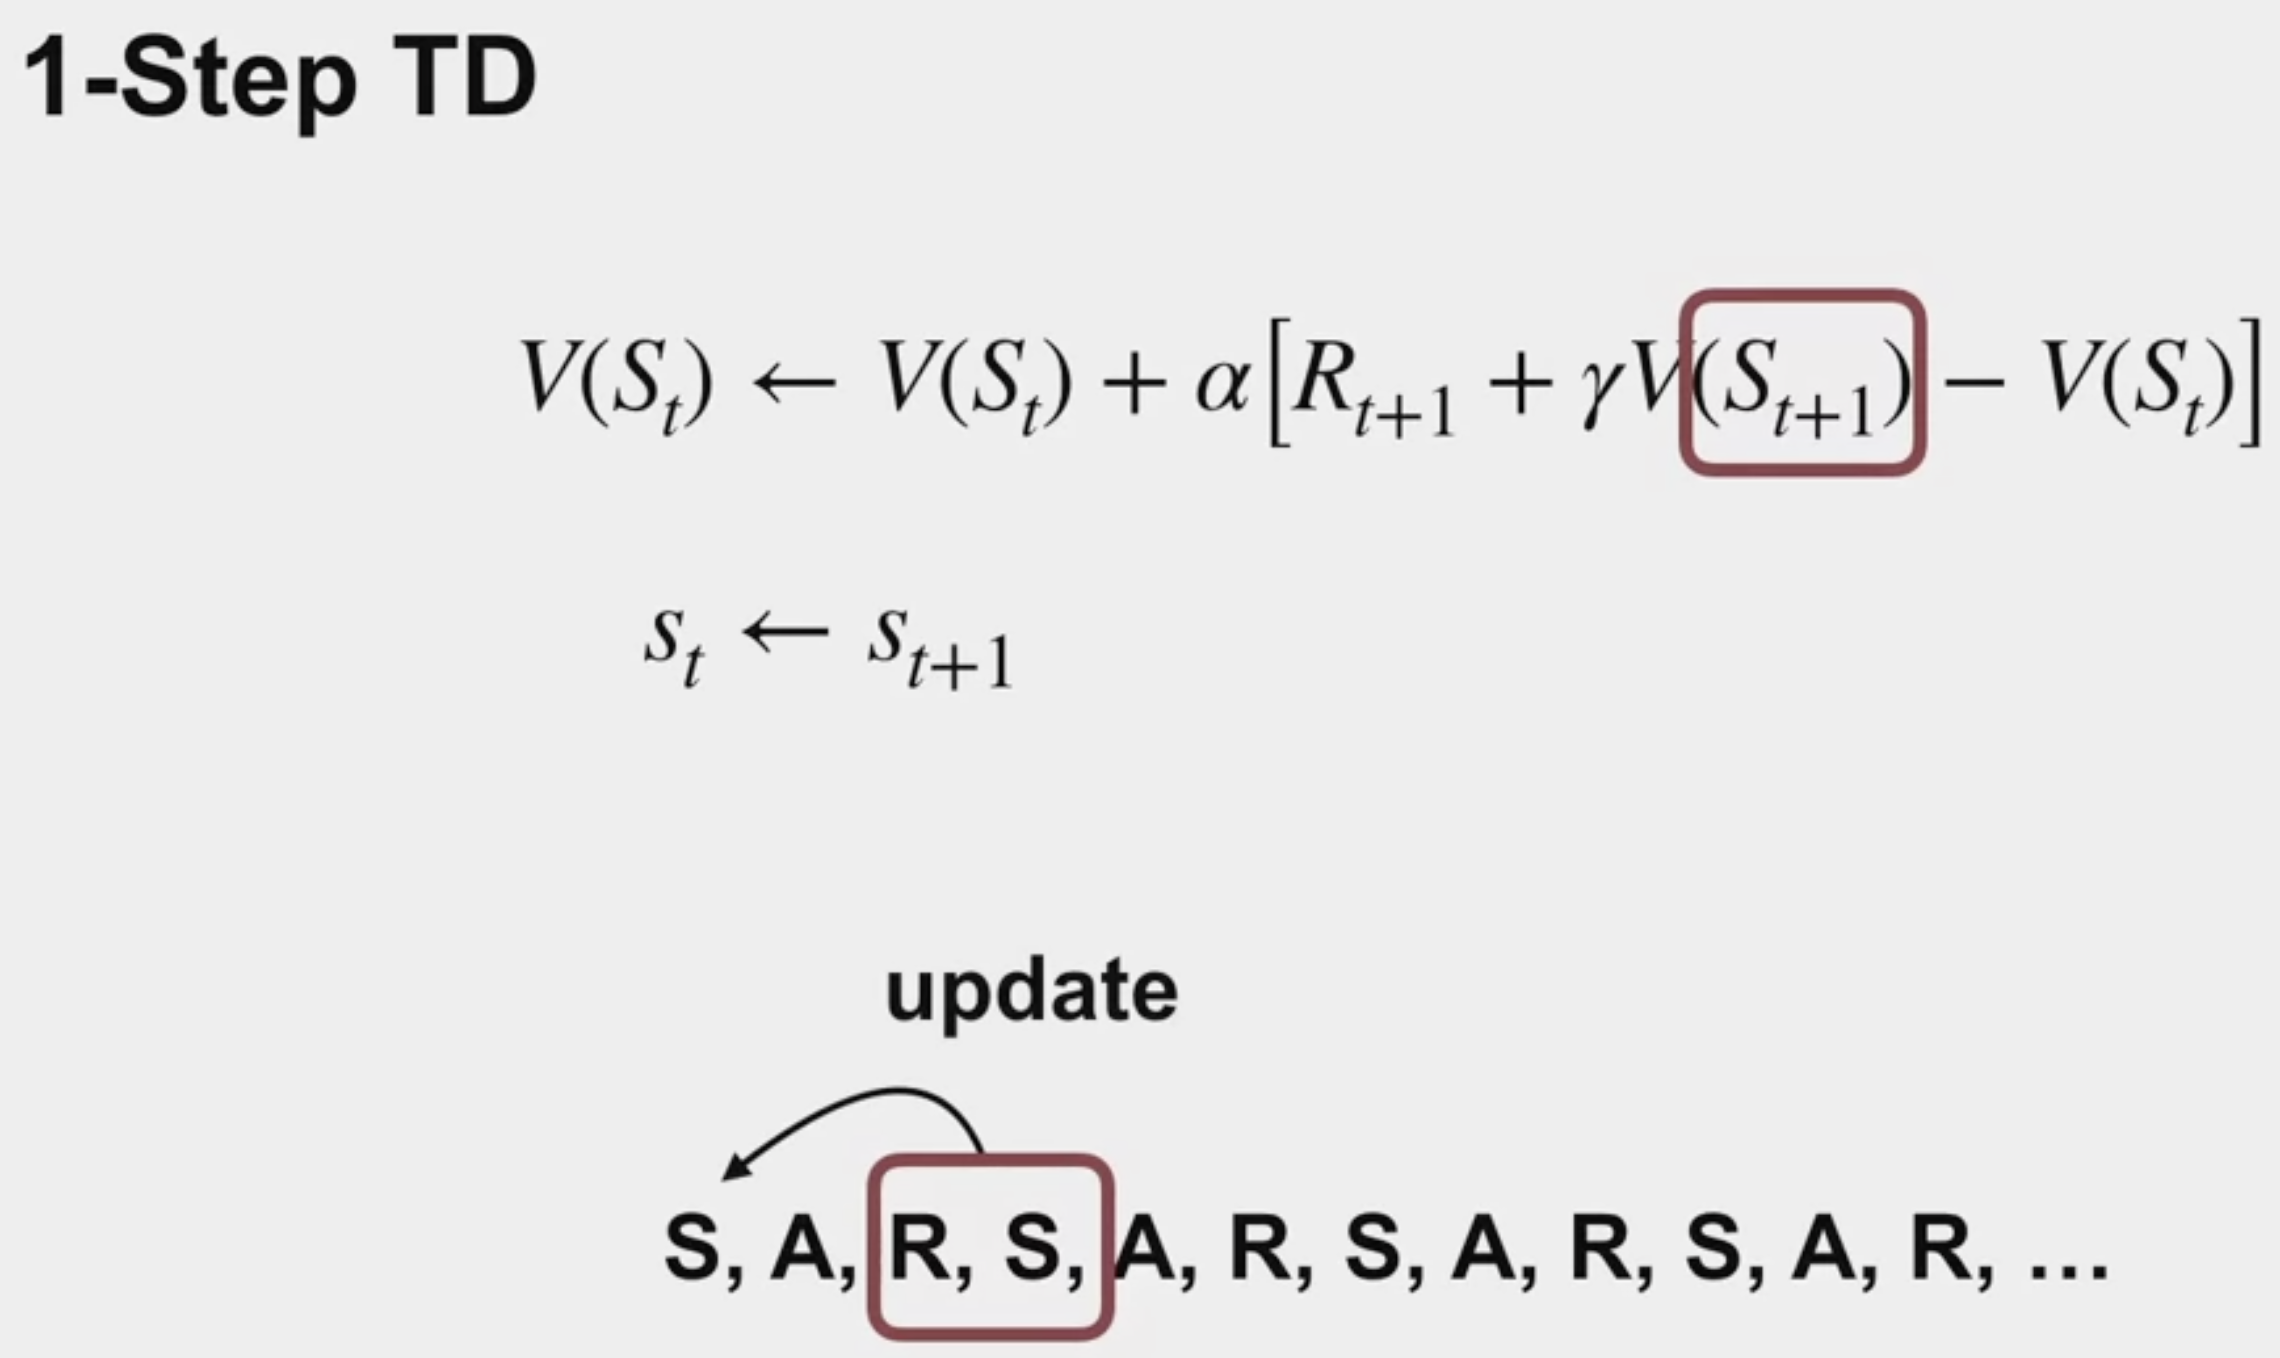
\includegraphics[width=0.7\columnwidth]{images/1-step-td.png}
        \caption{Illustration of 1-Step TD, TD(0)}
        \label{fig:1-step-td}
    \end{figure}
  \end{itemize}
\end{itemize}

\textbf{TD(0) a.k.a 1-Step TD}

So the simplest TD method (TD(0)) makes the update
$$V(S_t) \leftarrow V(S_t) + \alpha \underbrace{[\underbrace{R_{t+1} + \gamma V(S_{t+1})}_\text{t target} - V(S_t)]}_\text{TD-error $\delta_t$}$$
immediately on transition to $S_{t+1}$ and receiving $R_{t+1}$.

It is a special case of the $TD(\lambda)$ and $n$-step TD methods.

The below pseudocode specifies TD(0) completely in procedural form.



\begin{tcolorbox}[title={Tabular TD(0) for estimating $v_\pi$}]

\textbf{Input:} the policy $\pi$ to be evaluated

\textbf{Algorithm parameter:} step size $\alpha \in (0,1])$

\textbf{Initialize:} $V(s)$ for all $s \in \mathcal{S}^+$ arbitrarily except that $V (terminal) = 0$ \\

\textbf{Loop for each episode:}
\begin{description}
   \item $\;\;\;$ Initialize $S$
   \item $\;\;\;$ \textbf{Loop for each step of episode:}
   \begin{description}
     \item $\;\;\;$ $A \leftarrow$ action given by $\pi$ for $S$
     \item $\;\;\;$ Take action $A$ observe $R, S'$
     \item $\;\;\;$ $V(S) \leftarrow V(S) + \alpha [R + \gamma V(S') - V(S)]$
     \item $\;\;\;$ $S \leftarrow S'$
   \end{description}
   \item $\;\;\;$ \textbf{until $S$ is terminal}
\end{description}
\end{tcolorbox}






\subsection{Rich Sutton: The Importance of TD Learning}\label{the-importance-of-td-learning}


\textbf{\textcolor{blue}{Learning to predict (Prediction Learning}) is the single most scalable kind of learning.}

\begin{itemize}
  \item It is the \uline{unsupervised supervised learning}.
  \begin{itemize}
    \item We have a target (just by waiting)
    \item Yet no human labeling is needed!
  \end{itemize}
  \item Prediction learning is \uline{\textbf{scalable} model-free learning}.
\end{itemize}


\textbf{\textcolor{blue}{TD learning} is a method for \textcolor{blue}{learning to predict} from another, later, learned prediction.}

\begin{itemize}
  \item i.e. \textit{learnig a guess from guess}
  \item The TD error is the difference between the two predictions, the \textit{temporal difference}
  \item Otherwise TD learning is the same as supervised-learning, backpropagating the error
\end{itemize}


\textbf{\textcolor{blue}{TD learning} benefits and insights.}

\begin{itemize}
  \item Relevant only on \uline{\textit{multi-step} prediction problems} (everything other than the classical supervised learning setup)
  \begin{itemize}
    \item with information about it possibly revealed on each step
  \end{itemize}
  \item It is learning specialized for general, multi-step prediction, which may be key to perception, meaning, and modeling of the world
  \item It takes advantage of the \textbf{state property}
  \begin{itemize}
    \item which makes it \uline{fast, data efficient}
    \item which also makes it \uline{asymptotically biased}
  \end{itemize}
  \item It is \uline{computationally congenial}
  \item \textbf{Widely used in RL} to predict future rewards (value functions)
  \item \textbf{Key to} $Q$-learning, Sarsa, TD($\lambda$), Deep Q networks, TD-Gammon actor-critic methods, Samuel's checker player
  \begin{itemize}
    \item but not AlphaGo, helicopter autopilots, pure policy-based methods
  \end{itemize}
  \item Appears to be how brain reward systems work
  \item Can be used to predict any signal, not just rewards
\end{itemize}











\subsection{Advantages of TD Prediction Methods}\label{advantages-of-td-prediction-methods}


\begin{itemize}
  \item Unlike dynamic programming, TD methods \uline{do not require a model of the environment}.
  \item Unlike Monte Carlo, TD methods can \uline{learn online} (update the values on every step) without waiting to know the final outcome. Bootstrapping allows us to update the estimates based on other estimates.
  \item \uline{Converge faster than MC methods}.
\end{itemize}







\subsection{Optimality of TD(0)}\label{optimality-of-td(0)}

Under batch updating, TD(0) converges deterministically to a single answer independent of the step-size parameter, $\alpha$, as long as $\alpha$ is chosen to be sufficiently small.

The constant-$\alpha$ MC method also converges deterministically under the same conditions, but to a different answer.
\begin{itemize}
  \item Under batch training, constant-$\alpha$ MC converges to values, V(s), that are sample averages of the actual returns experienced after visiting each state s.
\end{itemize}

These are optimal estimates in the sense that they minimize the mean-squared error from the actual returns in the training set. In this sense it is surprising that the batch TD method was able to perform better according to the root mean-squared error measure shown in Figure \ref{fig:batch-training-td-vs-mc} below.

\begin{figure}[H]
  \centering
    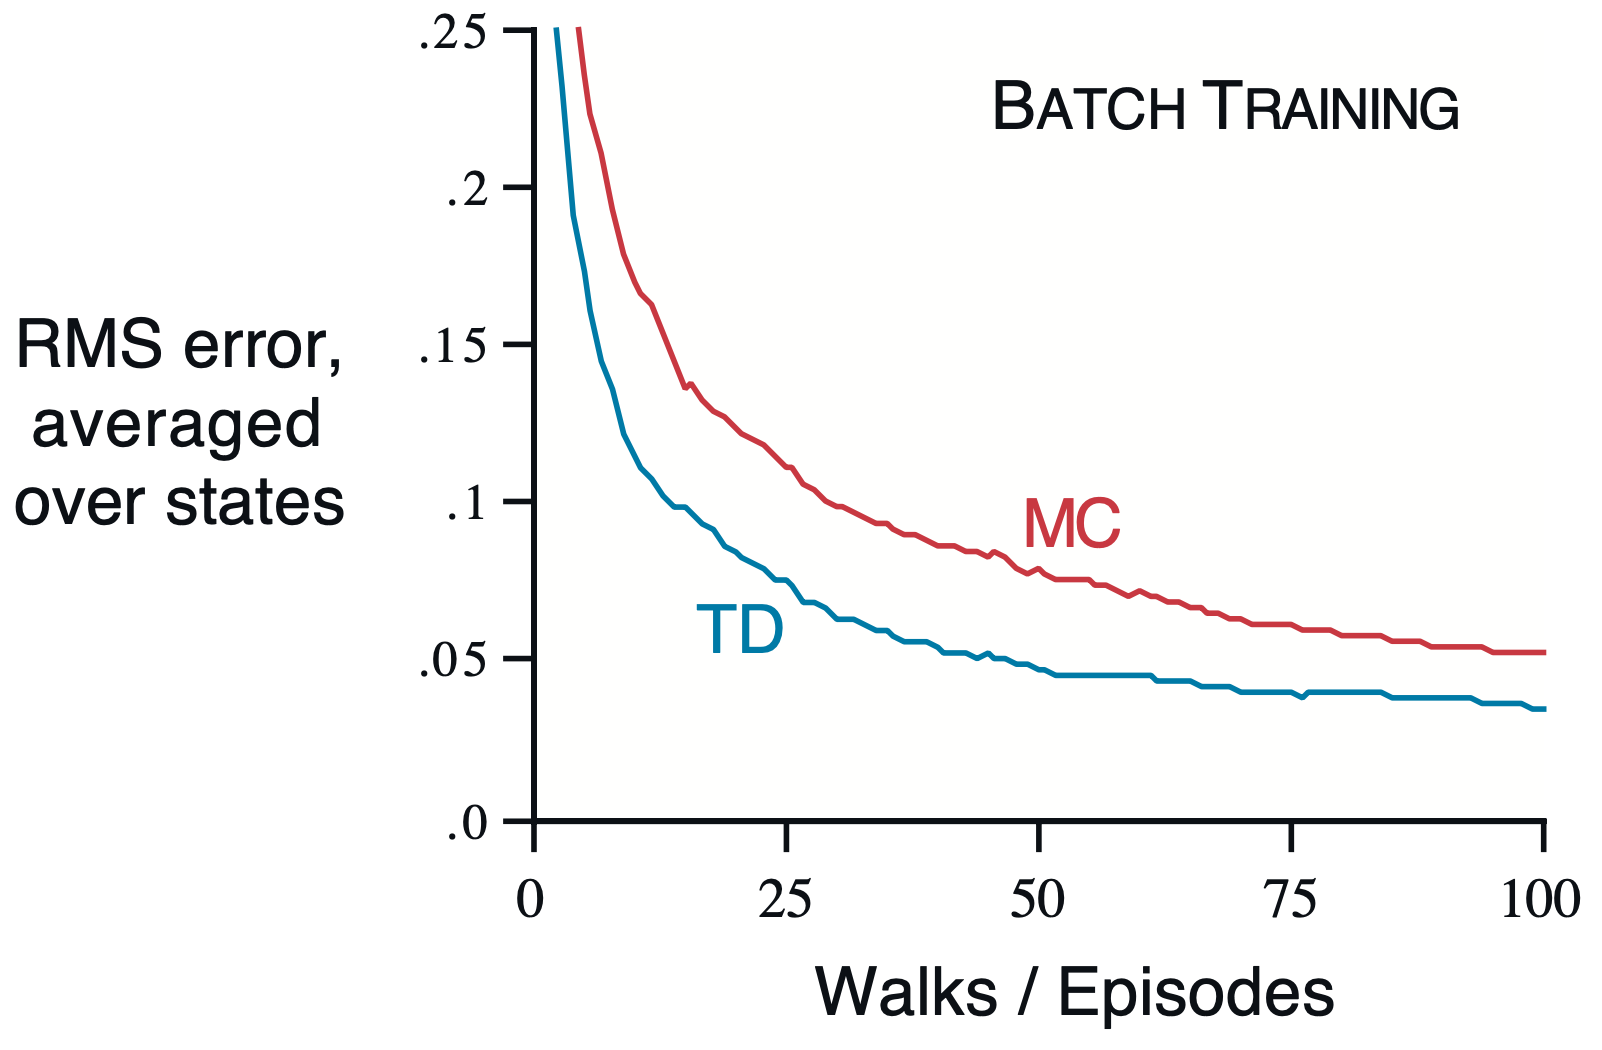
\includegraphics[width=0.6\columnwidth]{images/batch-training-td-vs-mc.png}
    \caption{Performance of TD(0) and constant-$\alpha$ MC under batch training on the random walk task}
    \label{fig:batch-training-td-vs-mc}
\end{figure}

The answer is that the Monte Carlo method is optimal only in a limited way, and
that \uline{TD is optimal in a way that is more relevant to predicting returns}.

On tasks with large state spaces, TD methods may be the only feasible way of approximating the certainty-equivalence solution.










\subsection{Sarsa: On-policy TD Control}\label{sarsa}

\textbf{What:} algorithm that perfrms on-policy TD control by learning an action-value function $q_\pi$.

The \textbf{\textcolor{blue}{SARSA}} acronym describes the data used in the updates:
\begin{itemize}
  \item \textbf{\textcolor{blue}{S}}tate, \textbf{\textcolor{blue}{A}}ction, \textbf{\textcolor{blue}{R}}eward, next \textbf{\textcolor{blue}{S}}tate, next \textbf{\textcolor{blue}{A}}ction.
  \item $S_t \;, \;\;\; A_t \;, \;\;\; R_{t+1} \;, \;\;\; S_{t+1} \;, \;\;\; A_{t+1}$
\end{itemize}


\textbf{\textcolor{blue}{Sarsa algorithm:}}

$$
Q(S_t, A_t) \leftarrow Q(S_t, A_t) + \alpha (R_{t+1} + \gamma Q(S_{t+1}, A_{t+1}) - Q(S_t, A_t))
$$

The general form of the Sarsa control algorithm is given in the box below.

\begin{tcolorbox}[title={Sarsa (on-policy TD control) for estimating $Q \approx q_*$}]

\textbf{Algorithm parameters:} $\alpha \in (0,1])$ \& small $\epsilon > 0$

\textbf{Initialize:} $Q(s, a)$ for all $s \in \mathcal{S}^+, a \in \mathcal{A}(s)$ arbitrarily except that $Q(terminal, \cdot) = 0$ \\

\textbf{Loop for each episode:}
\begin{description}
   \item $\;\;\;$ Initialize $S$
   \item $\;\;\;$ Choose $A$ from $S$ using policy derived from $Q$ (e.g. $\epsilon$-greedy)
   \item $\;\;\;$ \textbf{Loop for each step of episode:}
   \begin{description}
     \item $\;\;\;$ Take action $A$ observe $R, S'$
     \item $\;\;\;$ Choose $A'$ from $S'$ using policy derived from $Q$ (e.g. $\epsilon$-greedy)
     \item $\;\;\;$ $Q(S, A) \leftarrow Q(S, A) + \alpha [R + \gamma Q(S', A') - Q(S, A)]$
     \item $\;\;\;$ $S \leftarrow S'; A \leftarrow A'$
   \end{description}
   \item $\;\;\;$ \textbf{until $S$ is terminal}
\end{description}
\end{tcolorbox}

In Sarsa, the agent needs to know its next state action pair before updating its value estimates. That means it \uline{has to commit to its next action before the update}.

\textcolor{Green}{Sarsa converges with probability 1 to an optimal policy} and action-value function \textbf{as long as} \uline{all state-action pairs are visited an infinite number of times} and the \uline{policy converges in the limit to the greedy policy} (which can be arranged, for example, with "$\epsilon$-greedy policies by setting " = 1/t).














\subsection{Q-learning: Off-policy TD Control}\label{q-learning}

\textbf{What:} algorithm that perfrms off-policy TD control by learning an action-value function $q_\pi$.

\textbf{\textcolor{blue}{Q-learning algorithm:}}

$$
Q(S_t, A_t) \leftarrow Q(S_t, A_t) + \alpha (R_{t+1} + \gamma \max_a Q(S_{t+1}, a) - Q(S_t, A_t))
$$


\textcolor{blue}{\textbf{Sarsa}} vs. \textcolor{blue}{\textbf{Q-learning}}:

\begin{itemize}
  \item \textcolor{blue}{\textbf{Sarsa}} is a \uline{sample-based version of \textcolor{blue}{policy iteration} which uses \textcolor{blue}{Bellman equation} for action values, that each depend on a fixed policy}.
  \item \textcolor{blue}{\textbf{Q-learning}} is a \uline{sample-based version of \textcolor{blue}{value iteration} which iteratively applies the \textcolor{blue}{Bellman's Optimality Equation}}.
  \begin{figure}[H]
    \centering
      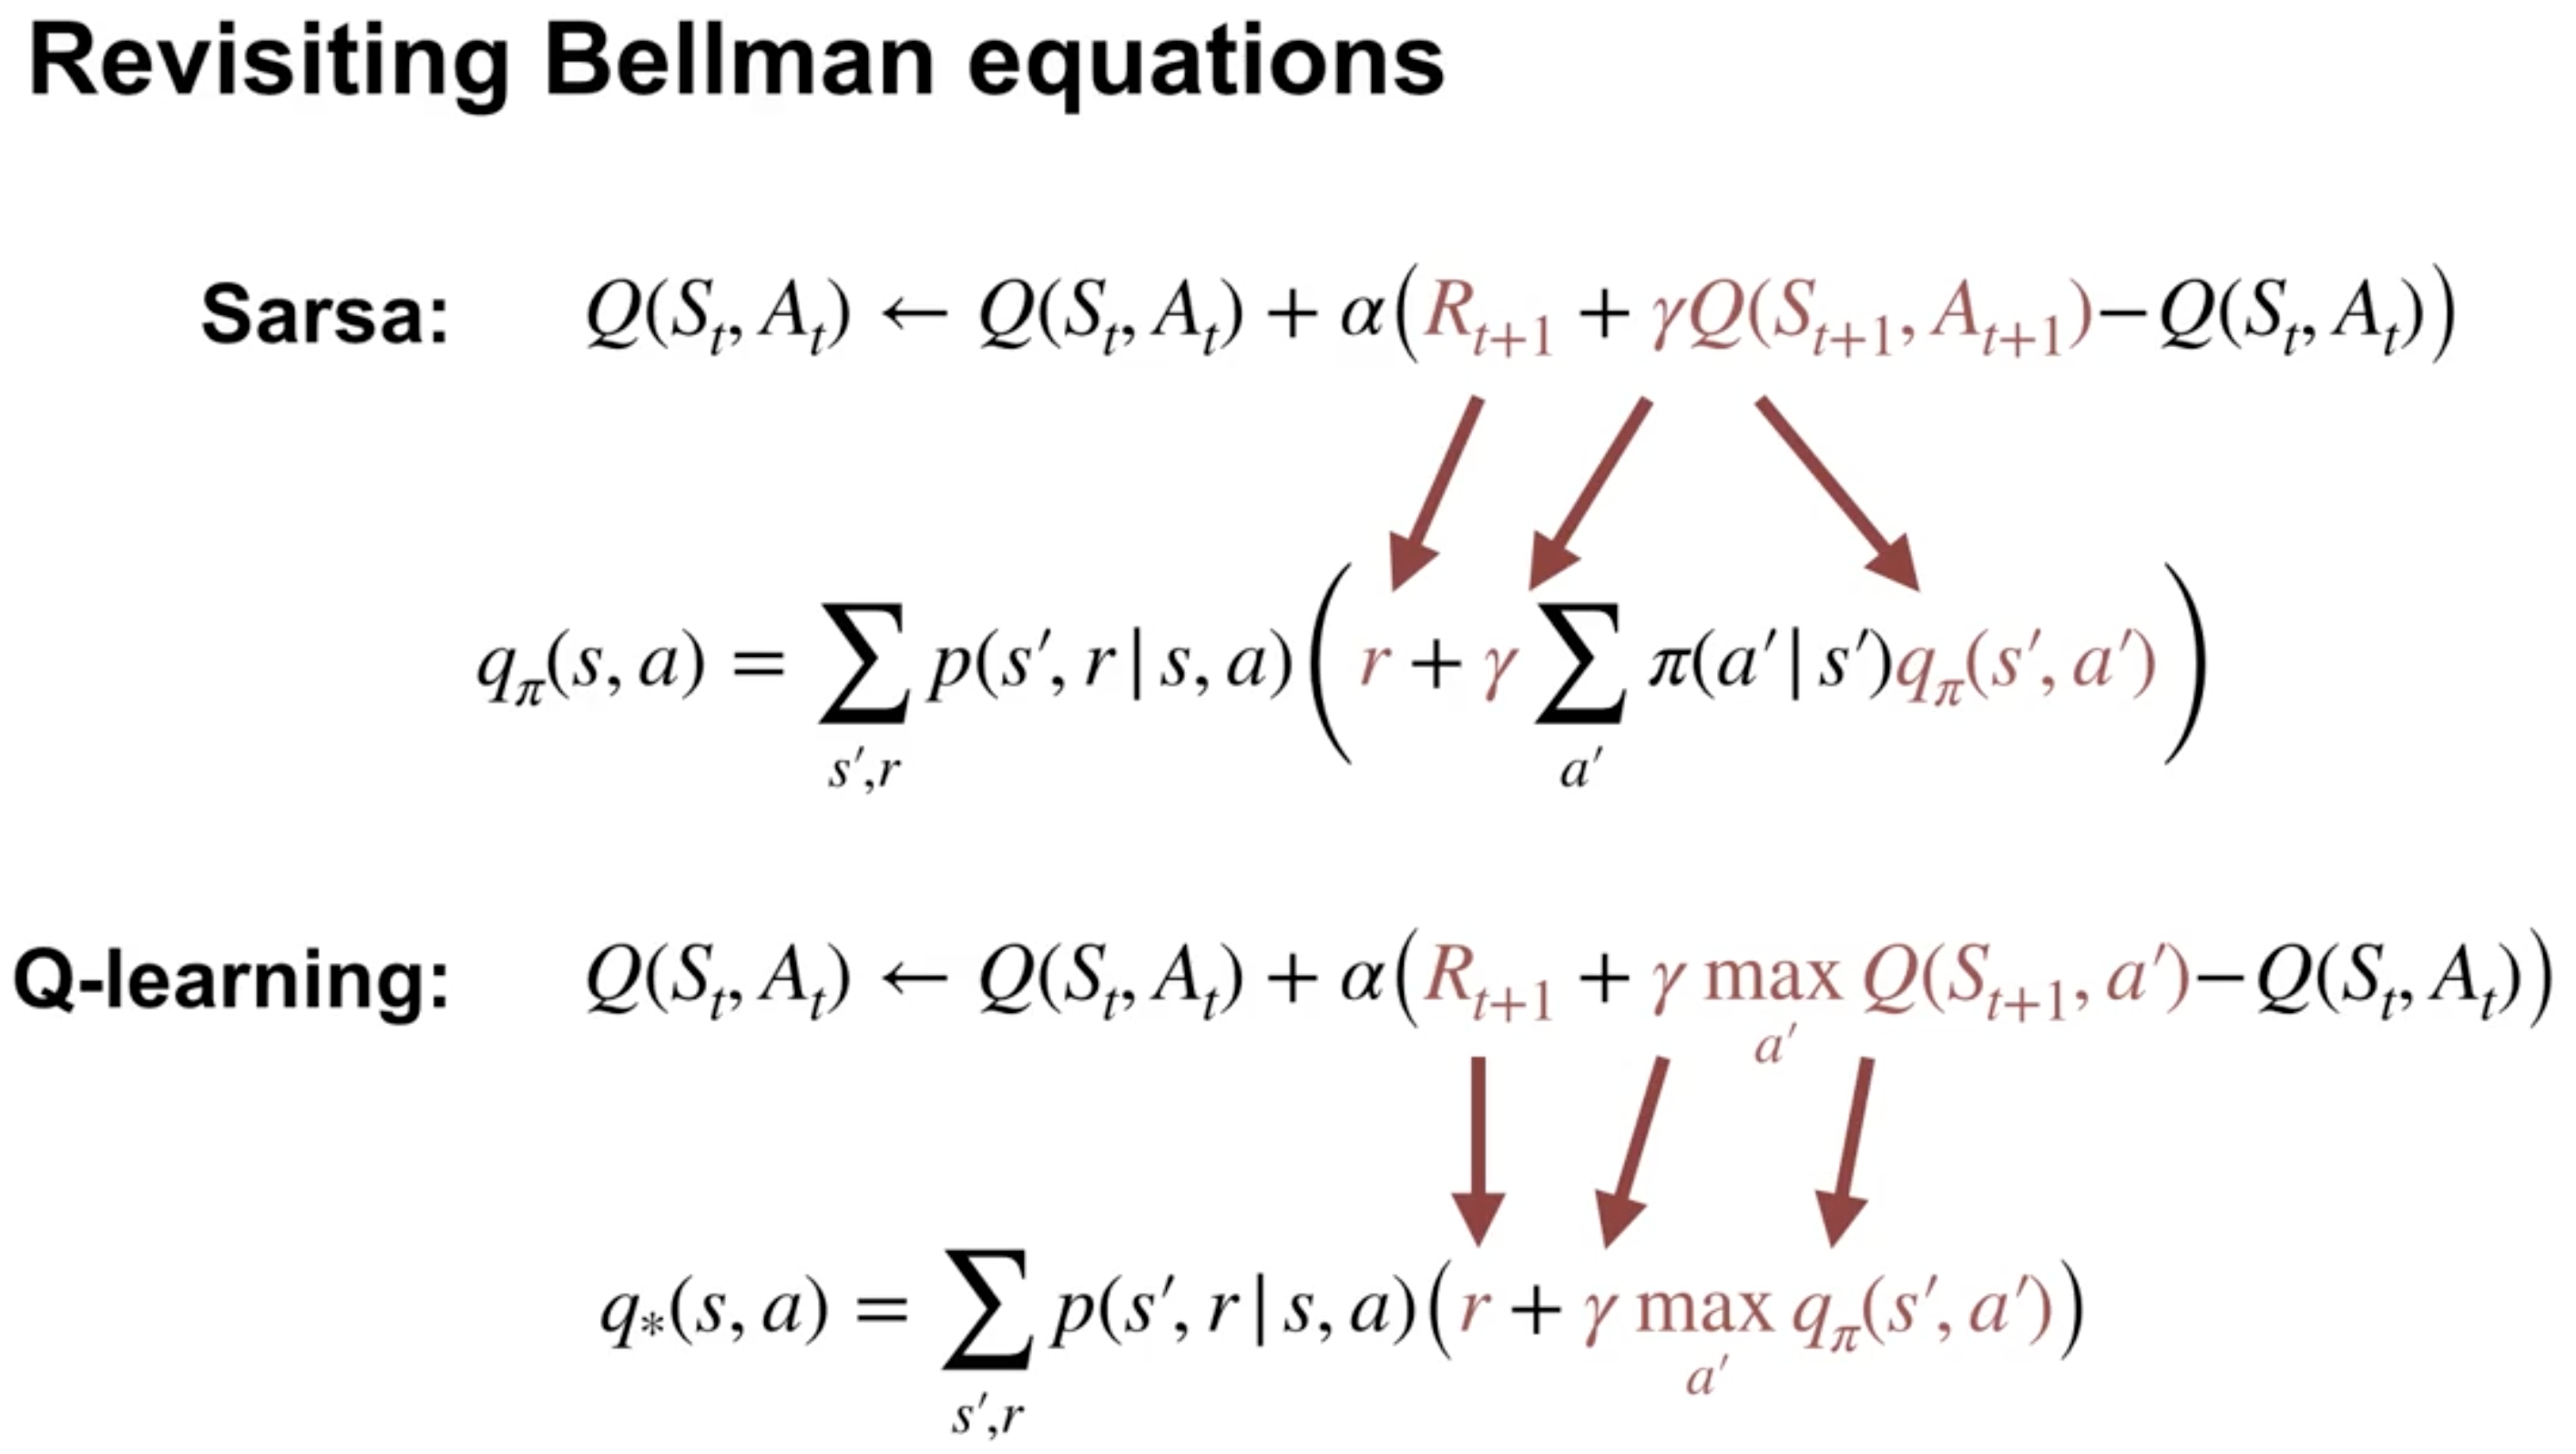
\includegraphics[width=0.8\columnwidth]{images/bellman-equation-sarsa-qlearning.png}
      \label{fig:bellman-equation-sarsa-qlearning}
  \end{figure}
  \item The optimality equations enable \textcolor{blue}{\textbf{Q-learning}} to \textcolor{Green}{directly learn Q-star instead of switching between policy improvement and policy evaluation steps}.
\end{itemize}


\begin{tcolorbox}[title={Q-learning (off-policy TD control) for estimating $\pi \approx \pi_*$}]

\textbf{Algorithm parameters:} step size $\alpha \in (0,1])$ \& small $\epsilon > 0$

\textbf{Initialize:} $Q(s, a)$ for all $s \in \mathcal{S}^+, a \in \mathcal{A}(s)$ arbitrarily except that $Q(terminal, \cdot) = 0$ \\

\textbf{Loop for each episode:}
\begin{description}
   \item $\;\;\;$ Initialize $S$
   \item $\;\;\;$ \textbf{Loop for each step of episode:}
   \begin{description}
     \item $\;\;\;$ Choose $A$ from $S$ using policy derived from $Q$ (e.g. $\epsilon$-greedy)
     \item $\;\;\;$ Take action $A$ observe $R, S'$
     \item $\;\;\;$ $Q(S, A) \leftarrow Q(S, A) + \alpha [R + \gamma \max_a Q(S', a) - Q(S, A)]$
     \item $\;\;\;$ $S \leftarrow S'$
   \end{description}
   \item $\;\;\;$ \textbf{until $S$ is terminal}
\end{description}
\end{tcolorbox}


\bigskip

\textbf{How is Q-learning off-policy?}
\begin{itemize}
  \item Since Q-learning \uline{learns about the best action it could possibly take rather than the actions it actually takes}, it is learning off-policy.
  \item \textbf{Why no important sampling ratios (with 1-step)?} Because the agent is estimating action values with unknown policy. It does not need important sampling ratios to correct for the difference in action selection. The action value function represents the returns following each action in a given state. The agents target policy represents the probability of taking each action in a given state. Putting these two elements together, the agent can calculate the expected return under its target policy from any given state, in particular, the next state, $S_{t+1}$.

\end{itemize}

\textcolor{Green}{Q-learning also converges to the optimal value function} as long as the aging continues to explore and samples all areas of the state action space.











\subsection{Expected Sarsa}\label{expected-sarsa}

The algorithm is nearly identical to Sarsa, except the TD error uses the expected estimate of the next action value instead of a sample of the next action value.
\begin{itemize}
  \item Sarsa:
  $$
  Q(S_t, A_t) \leftarrow Q(S_t, A_t) + \alpha (R_{t+1} + \gamma \textcolor{purple}{Q(S_{t+1}, A_{t+1})} - Q(S_t, A_t))
  $$
  \item Expected Sarsa:
  \begin{align*}
    Q(S_t, A_t) &\leftarrow Q(S_t, A_t) + \alpha (R_{t+1} + \gamma \textcolor{purple}{\mathbb{E}_\pi [Q(S_{t+1}, A_{t+1}) | S_{t+1}]} - Q(S_t, A_t)) \\
    &\leftarrow Q(S_t, A_t) + \alpha (R_{t+1} + \gamma \textcolor{purple}{\sum_{a'} \pi(a' | S_{t+1}) Q(S_{t+1}, a')} - Q(S_t, A_t))
  \end{align*}
\end{itemize}


\textbf{Motivation:} Sarsa estimates this expectation by sampling the next date from the environment and the next action from its policy. But the agent already knows this policy, so why should it have to sample its next action? Instead, it should just compute the expectation directly.

\textbf{Expected Sarsa vs. Sarsa (Pross \& Cons)}
\begin{itemize}
  \item There's a huge upside to calculating the expectation explicitly: Expected Sarsa has a \textcolor{Green}{more stable update target} than Sarsa.
  \item The lower variance comes with a downside though. Computing the average over next actions becomes \textcolor{red}{more expensive as the number of actions increases}. When there are many actions, computing the average might take a long time, especially since the average has to be computed every time step.
  \item Expected Sarsa is \textcolor{Green}{more robust} than Sarsa \textcolor{Green}{to large step sizes}.
\end{itemize}

Expected Sarsa can do off-policy learning without using importance sampling.

Expected Sarsa with greedy target policy $\equiv (equivalent\;to)$ Q-Learning
\begin{itemize}
  \item[$\rightarrow$] Q-Learning is a special case of Expected Sarsa.
  \item Expected Sarsa can also do off-policy learning without using importance sampling.
\end{itemize}


















\section{$n$-step Bootstrapping}\label{nstep-bootstrapping}

\begin{tcolorbox}[colback=yellow!5,colframe=yellow!75!black,title=NOTE]
  \textbf{Idea of $n$-step methods} is \textcolor{Orange}{usually used as an \uline{introduction to the algorithmic idea of \textit{eligibility traces} (Chapter 12)}}, which enable bootstrapping over multiple time intervals simultaneously. \textbf{Here} we instead consider the n-step bootstrapping idea on its own.
\end{tcolorbox}


\textbf{What:} methods that \uline{unifies \textcolor{blue}{MC} \& \textcolor{blue}{TD(0)} methods} so that one can shift from one to the other smoothly as needed to meet the demands of a particular task.

\textbf{Motivation:} Neither \textcolor{blue}{MC} methods nor \textcolor{blue}{one-step TD} methods are always the best. The \textcolor{Green}{best methods are often intermediate between the two extremes}.

\begin{figure}[H]
  \centering
    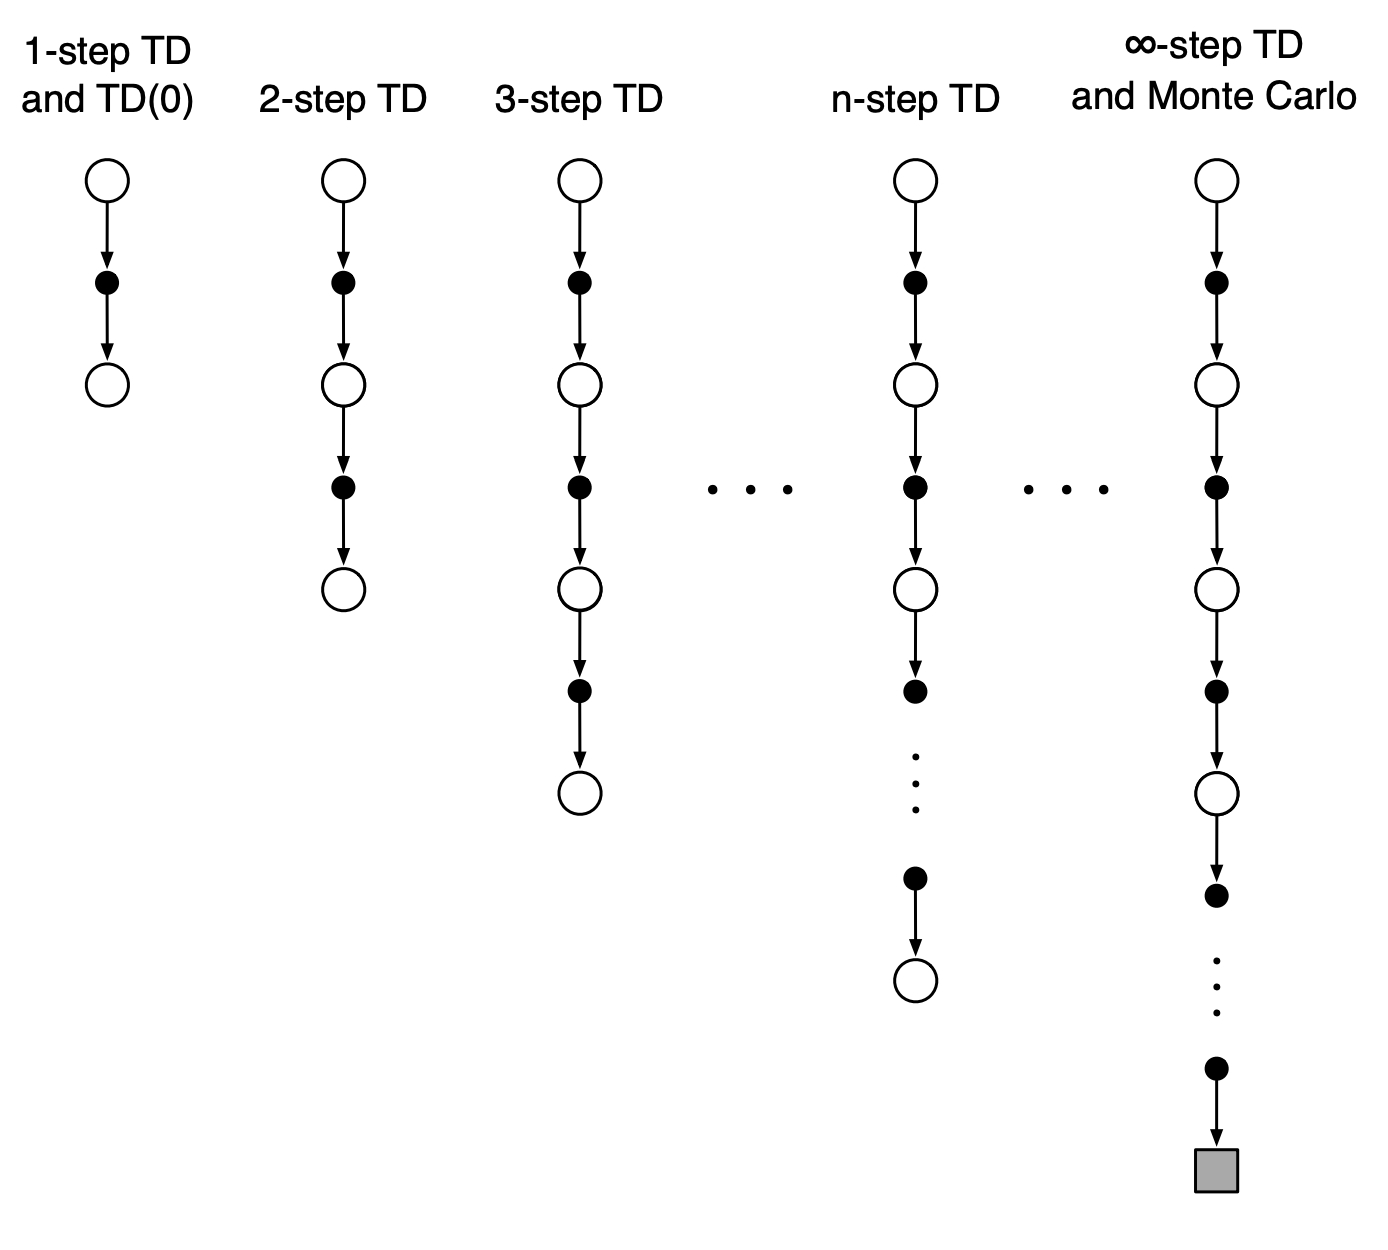
\includegraphics[width=0.9\columnwidth]{images/n-step-methods.png}
    \caption{These $n$-step methods form a spectrum ranging from one-step TD methods to Monte Carlo methods.}
    \label{fig:n-step-methods}
\end{figure}


\textbf{How they work:}
\begin{itemize}
  \item $n$-step TD will perform an update based on the next $n$ rewards, and the estimated value of the corresponding state ($n$ steps ahead).
\end{itemize}

\textbf{Returns of the method on the spectrum:}
\begin{itemize}
  \item \textbf{Monte Carlo} updates the estimate of $v_\pi(S_t)$ is updated in the direction of the \uline{complete return}:
  \begin{gather*}
    G_{t} \doteq R_{t+1} + \gamma R_{t+2} + \gamma^2 R_{t+3} + ... + \gamma^{T-t-1} R_{T} \\ \\
    \textbf{Where:} \\
    T\text{: is the last time step of the episode} \\
  \end{gather*}
  \begin{itemize}
    \item Let us call this quantity the \textit{target} of the update.
  \end{itemize}
  \item All \textbf{$n$-step returns} can be considered \uline{approximations to the full return}, truncated after n steps and then corrected for the remaining missing terms by $V_{t+n-1}(S_{t+n})$.
  \begin{itemize}
    \item Return in 1-step TD method:
    $$
    G_{t:t+1} \doteq R_{t+1} + \gamma V_{t}(S_{t+1})
    $$
    \item Return in 2-step TD method:
    $$
    G_{t:t+2} \doteq R_{t+1} + \gamma R_{t+2} + \gamma^2 V_{t+1}(S_{t+2})
    $$
    \item Return in $n$-step TD method:
    $$
    G_{t:t+n} \doteq R_{t+1} + \gamma R_{t+2} + ... + \gamma^{n-1} R_{t+n} + \gamma^{n} V_{t+n-1}(S_{t+n})
    $$
    \item If $t+n \leq T$ (if the $n$-step return extends to or beyond termination), then all the missing terms are taken as zero, and the $n$-step return defined to be equal to the ordinary full return ($G_{t:t+n} \doteq G_t \text{ if } t+n \geq T$).
  \end{itemize}
\end{itemize}


\textbf{$n$-step TD Algorithm:}
\begin{itemize}
  \item No real algorithm can use the $n$-step return until after it has seen $R_{t+n}$ and computed $V_{t+n-1}$. The first time these are available is $t+n$. The natural state-value learning algorithm for using $n$-step returns is thus
  $$
  V_{t+n}(S_t) \doteq V_{t+n-1}(S_t) + \alpha (G_{t:t+n} - V_{t+n-1}(S_t)), \;\;\;\; 0 \leq t < T,
  $$
  \item while the values of all other states remain unchanged: $V_{t+n}(s) = V_{t+n-1}(s)$, for all $s \neq S_t$.
\end{itemize}
















\section{Planning and Learning with Tabular Methods (Model based RL)}\label{planning-and-learning-with-tabular-methods}

We've seen:
\begin{itemize}
  \item sample-based methods like TD which learn only from sampled experience.
  \item dynamic programming methods which plan by using complete information about how things work, without having to make decisions.
\end{itemize}
It would be even better if we could obtain an intermediate method that can leverage the best of both extremes.

So far, we’ve used off-policy learning to facilitate exploration in a problem that has one goal. But actually you can use off-policy learning to learn how to get to many different goals.






\subsection{Models and Planning}\label{models-and-planning}


\textbf{\textcolor{blue}{Model:}} is used to \uline{store knowledge about the dynamics}. It should produce a possible next state and reward. This allows us to see an outcome of an action without having to actually take it.

\begin{figure}[H]
  \centering
    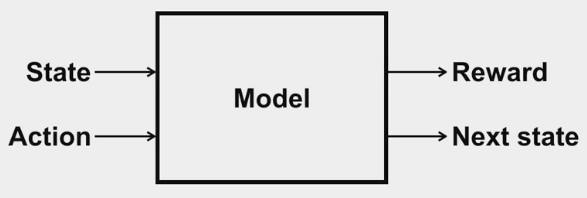
\includegraphics[width=0.6\columnwidth]{images/model.png}
    \label{fig:model}
\end{figure}

\begin{itemize}
  \item \textbf{\textcolor{blue}{Planning}} refers to the process of \uline{using a \textcolor{blue}{model} to improve a policy (with simulated experience)}. One way is to:
  \begin{enumerate}
    \item Simulate experience (sample experience from the model)
    \begin{itemize}
      \item Simulating experience improves the sample efficiency. The addition of simulated experience means the agent needs fewer interactions with the world to come up with the same policy.
    \end{itemize}
    \item Perform value function updates as if those experiences happened
    \item Behaving greedily with respect to these improved values results in improved policy.
    \begin{figure}[H]
      \centering
        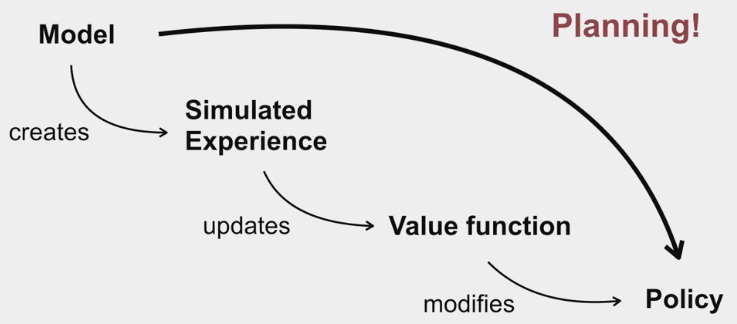
\includegraphics[width=0.8\columnwidth]{images/planning.png}
        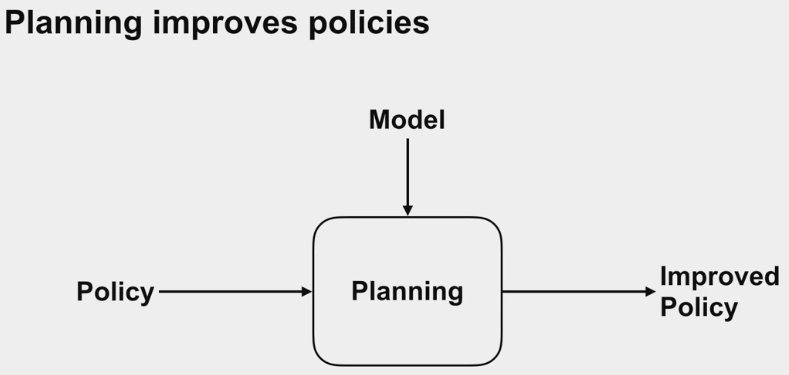
\includegraphics[width=0.8\columnwidth]{images/planning2.png}
        \label{fig:planning}
    \end{figure}
  \end{enumerate}
\end{itemize}




\textbf{\textcolor{blue}{Types of Models:}}
\begin{itemize}
  \item \textbf{\textcolor{blue}{Sample Model:}} produces an actual outcome drawn from some underlying probabilities. They generate samples without explicitly storing the probability of each outcome.
  \begin{itemize}
    \item \textbf{\textcolor{Green}{Pros} \& \textcolor{red}{Cons}:}
    \begin{itemize}
      \item[\textcolor{Green}{$+$}] require \textcolor{Green}{less memory / computationally inexpensive} (because random outcomes can be produced according to a set of rules)
      \item[\textcolor{red}{$-$}] can \textcolor{red}{only approximate expected outcome}
    \end{itemize}
  \end{itemize}
  \item \textbf{\textcolor{blue}{Distribution Model:}} completely specifies the likelihood or probability of every outcome.
  \begin{itemize}
    \item \textbf{\textcolor{Green}{Pros} \& \textcolor{red}{Cons}:}
    \begin{itemize}
      \item can \textcolor{Green}{compute the exact expected outcome} (by summing over all outcomes weighted by their probabilities). These \textcolor{Green}{can be used to assess risk}.
      \item \textcolor{red}{can be difficult to specify} and \textcolor{red}{can become very large}
    \end{itemize}
  \end{itemize}
\end{itemize}




\textbf{\textcolor{blue}{Random-sample one-step tabular Q-planning:}}

\begin{itemize}
  \item Process:
  \begin{figure}[H]
    \centering
      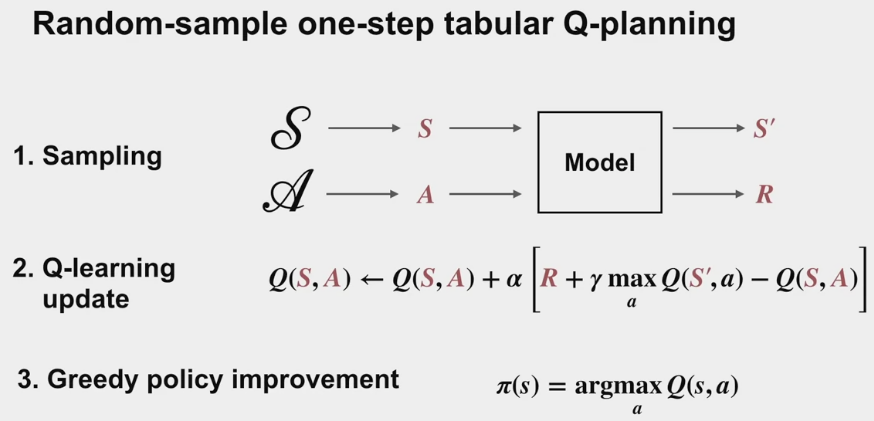
\includegraphics[width=0.8\columnwidth]{images/random-sample-one-step-tabular-q-learning.png}
      \label{fig:random-sample-one-step-tabular-q-learning}
  \end{figure}
  \item Assumptions:
  \begin{itemize}
    \item we have a sample model of the transition dynamics.
    \item we have a strategy for sampling relevant state action pairs
    \begin{figure}[H]
      \centering
        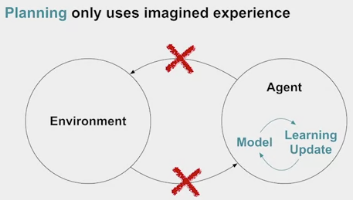
\includegraphics[width=0.5\columnwidth]{images/planning3.png}
        \label{fig:planning3}
    \end{figure}
  \end{itemize}
  \item Connection with Q-learning:
  \begin{itemize}
    \item Recall that \textbf{Q-learning} uses \uline{experienced from the environment}, they performs an update to improve a policy.
    \item In \textbf{Q-planning}, we use \uline{experience from the model} and perform a similar update to improve a policy.
  \end{itemize}
\end{itemize}












\subsection{Dyna (Architecture): Integrated Planning, Acting, and Learning}\label{dyna}

\textbf{What:} one way to \textbf{combine} \uline{direct RL updates} and \uline{planning updates}.


\textbf{\textcolor{blue}{Dyna Architecture:}}
\begin{figure}[H]
  \centering
    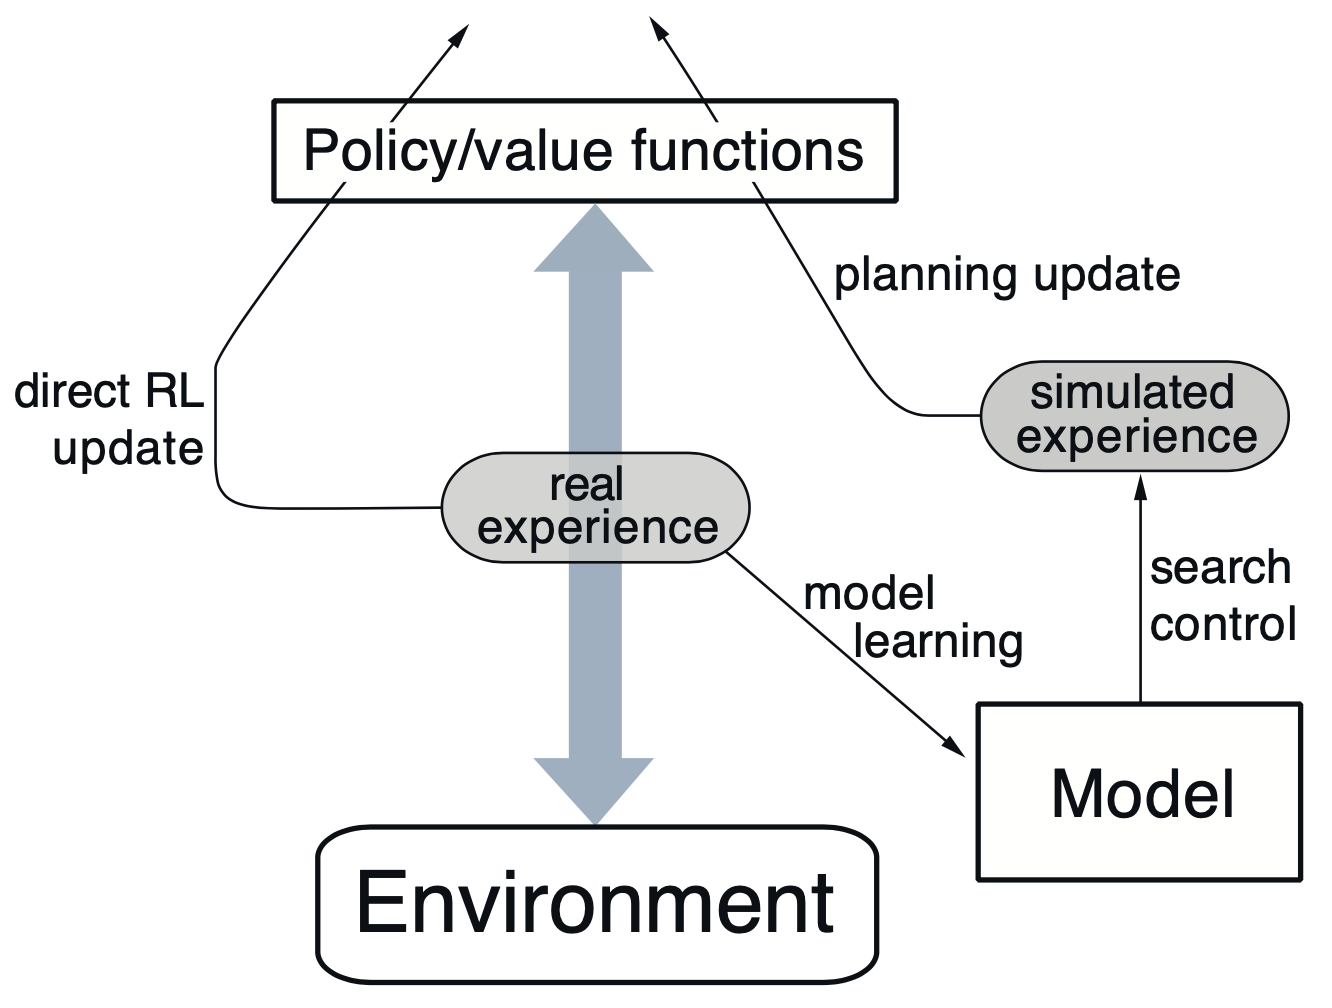
\includegraphics[width=0.8\columnwidth]{images/dyna-architecture.png}
    \label{fig:dyna-architecture}
\end{figure}
\begin{itemize}
  \item \textbf{Search control:} controlling how the model generates simulated experience, what states the agent will plan from (most be something the agent has seen before, otherwise the model wouldn't know what happens next).
\end{itemize}


\textbf{Example:} Agent learning path without vs. with (n) planning steps:
\begin{figure}[H]
  \centering
    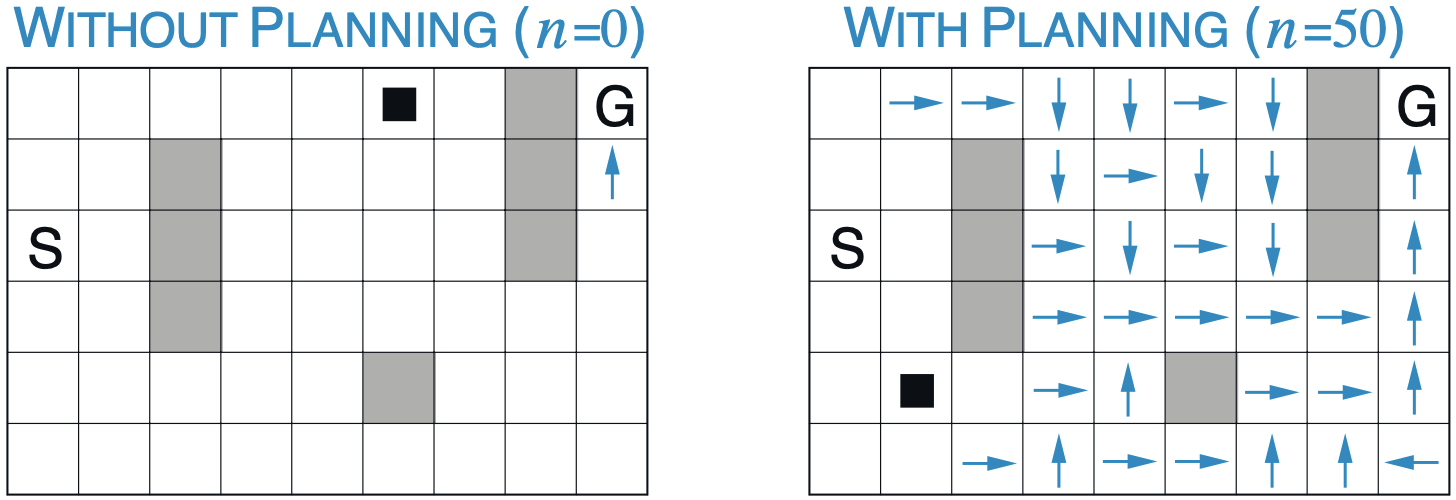
\includegraphics[width=0.8\columnwidth]{images/planning-vs-not.png}
    \caption{Policies found by planning and nonplanning Dyna-Q agents halfway through the second episode.}
    \label{fig:planning-vs-not}
\end{figure}


Pseudocode algorithm for Dyna-Q:

\begin{tcolorbox}[title={Tabular Dyna-Q}]

\textbf{Initialize:} $Q(s, a)$ and $Model(s, a)$ for all $s \in \mathcal{S}, a \in \mathcal{A}(s)$ \\

\textbf{Loop forever:}
\begin{itemize}
   \item[(a)] $\;\;\;$ $S \leftarrow$ current (nonterminal) state
   \item[(b)] $\;\;\;$ $A \leftarrow \epsilon$-greedy$(S,Q)$
   \item[(c)] $\;\;\;$ Take action $A$ observe $R, S'$
   \item[(d)] $\;\;\;$ $Q(S, A) \leftarrow Q(S, A) + \alpha [R + \gamma \max_a Q(S', a) - Q(S, A)]$
   \item[(e)] $\;\;\;$ $Model(S, A) \leftarrow R, S'$ (assuming deterministic environment)
   \item[(f)] $\;\;\;$ \textbf{Loop repeat $n$ times:}
   \begin{description}
     \item $\;\;\;$ $S \leftarrow$ random previously observed state
     \item $\;\;\;$ $A \leftarrow$ random action previously taken in $S$
     \item $\;\;\;$ $R,S' \leftarrow Model(S, A)$
     \item $\;\;\;$ $Q(S, A) \leftarrow Q(S, A) + \alpha [R + \gamma \max_a Q(S', a) - Q(S, A)]$
   \end{description}
\end{itemize}
\end{tcolorbox}

Dyna-Q is more sample efficient than Q-learning










\subsection{When the Model Is Wrong / Inaccurate}\label{wrong-model}

Models are inaccurate when transitions they store are different from transitions that happen in the environment.

\textbf{How models can be \textcolor{red}{inaccurate}:}
\begin{itemize}
  \item \textbf{\textcolor{red}{Incomplete model}:} At the beginning of learning, the agent hasn't tried most of the actions in almost all of the states. $\rightarrow$ Transitions associated with trying those actions in those states are simply missing from the model.
  \item \textbf{\textcolor{red}{Changing environment}:} Taking an action in a state could result in a different next state and reward than what the agent observed before the change.
\end{itemize}

Planning with an inaccurate model improves the policy or value function with respect to the model and not the environment.

Dyna-Q can plan with an incomplete model by only sampling state action pairs that had been previously visited.





\textbf{\textcolor{blue}{Dyna-$Q^+$ algorithm:}} uses a reward bonus in its planning updates to encourage exploration. By exploring, Dyna-$Q^+$ keeps its model up-to-date and accurate, resulting in better performance.

\begin{gather*}
\text{New reward} = r + \textcolor{blue}{\kappa + \sqrt{\tau}} \\ \\
  \textbf{Where:} \\
  r \text{: actual reward} \\
  \tau \text{: time step since transition was last tried} \\
  \kappa  \text{: small constant that controls the influence of the} \\ \text{bonus on the planning update}
\end{gather*}

\begin{figure}[H]
  \centering
    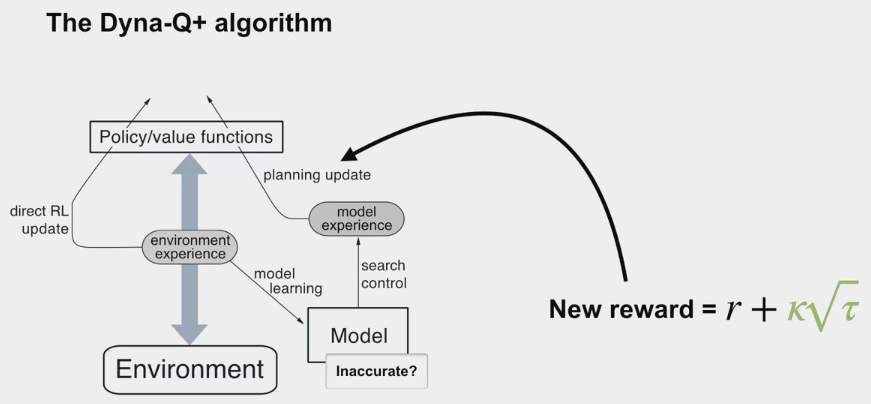
\includegraphics[width=0.9\columnwidth]{images/dyna-q-plus.png}
    \label{fig:dyna-q-plus}
\end{figure}










































\newpage
\part{Approximate Solution methods}\label{approximate-solution-methods}


In this part we describe how to \textbf{apply RL for arbitrarily large state spaces}. In many of our target tasks, almost every state encountered will never have been seen before. To make sensible decisions in such states it is necessary to \uline{\textit{generalize}} from previous encounters with different states that are in some sense similar to the current one. We can use \uline{\textit{function approximation} (instance of \textit{supervised learning}) for this task}.


In such cases we \textcolor{red}{cannot expect to find an optimal policy} or the optimal value function even in the limit of infinite time and data; our \textbf{goal instead} is to \uline{find a good approximate solution} using limited computational resources.




This involves a number of new issues that do not normally arise in conventional supervised learning, such as nonstationarity, bootstrapping, and delayed targets. We introduce these and other issues successively over the five chapters of this part



\textbf{Chapters in this section:}

\begin{itemize}
  \item Initially we restrict attention to \textbf{on-policy} training:
  \begin{itemize}
    \item[9.] On-policy \textbf{prediction} case (policy is given and only its value function is approximated)
    \item[10.] On-policy \textbf{control} case (approximation to the optimal policy is found)
  \end{itemize}
  \item[11.] \textbf{Off-policy} learning with function approximation
  \item[12.] Introducing and analyzing the algorithmic mechanism of \textbf{eligibility traces}, which \uline{dramatically improves the computational properties} of multi-step reinforcement learning methods in many cases.
  \item[13.] Exploring a \uline{different approach to control}, \textbf{policy-gradient methods}, which approximate the optimal policy directly and need never form an approximate value function (although they may be much more efficient if they do approximate a value function as well the policy).
\end{itemize}


\begin{center}\rule{0.5\linewidth}{0.5pt}\end{center}
\newpage



























\section{On-policy Prediction with Approximation}\label{on-policy-prediction-with-approximation}


Function approximation in reinforcement learning by considering its use in estimating the state-value function from on-policy data.



\subsection{Value-function Approximation}\label{value-function-approximation}


Function approximation methods expect to receive examples of the desired input–output behavior of the function they are trying to approximate. We use these methods for value prediction simply by passing to them the $s \rightarrow u$ ($s$ should be more like $u$) of each update as a training example. We then interpret the approximate function they produce as an estimated value function.


Supervised methods in value approximation:
\begin{itemize}
  \item must be able to \uline{learn online}
  \item must \uline{handle nonstationary target functions} (target functions that change over time)
\end{itemize}



\textbf{\textcolor{blue}{Generalization} in the context of policy evaluation} means that \uline{updates to the value estimate of one state influence the value of other states}.

\begin{itemize}
  \item Benefits:
  \begin{itemize}
    \item can speed learning by making better use of the experience we have $\rightarrow$ we may not have to visit every state as much to get this values correct if we can learn its value from similar states
  \end{itemize}
\end{itemize}


\textbf{\textcolor{blue}{Discrimination} in the context of policy evaluation} means the \uline{ability to make the values for two states different to distinguish between the values for these two states}.



\begin{figure}[H]
  \centering
    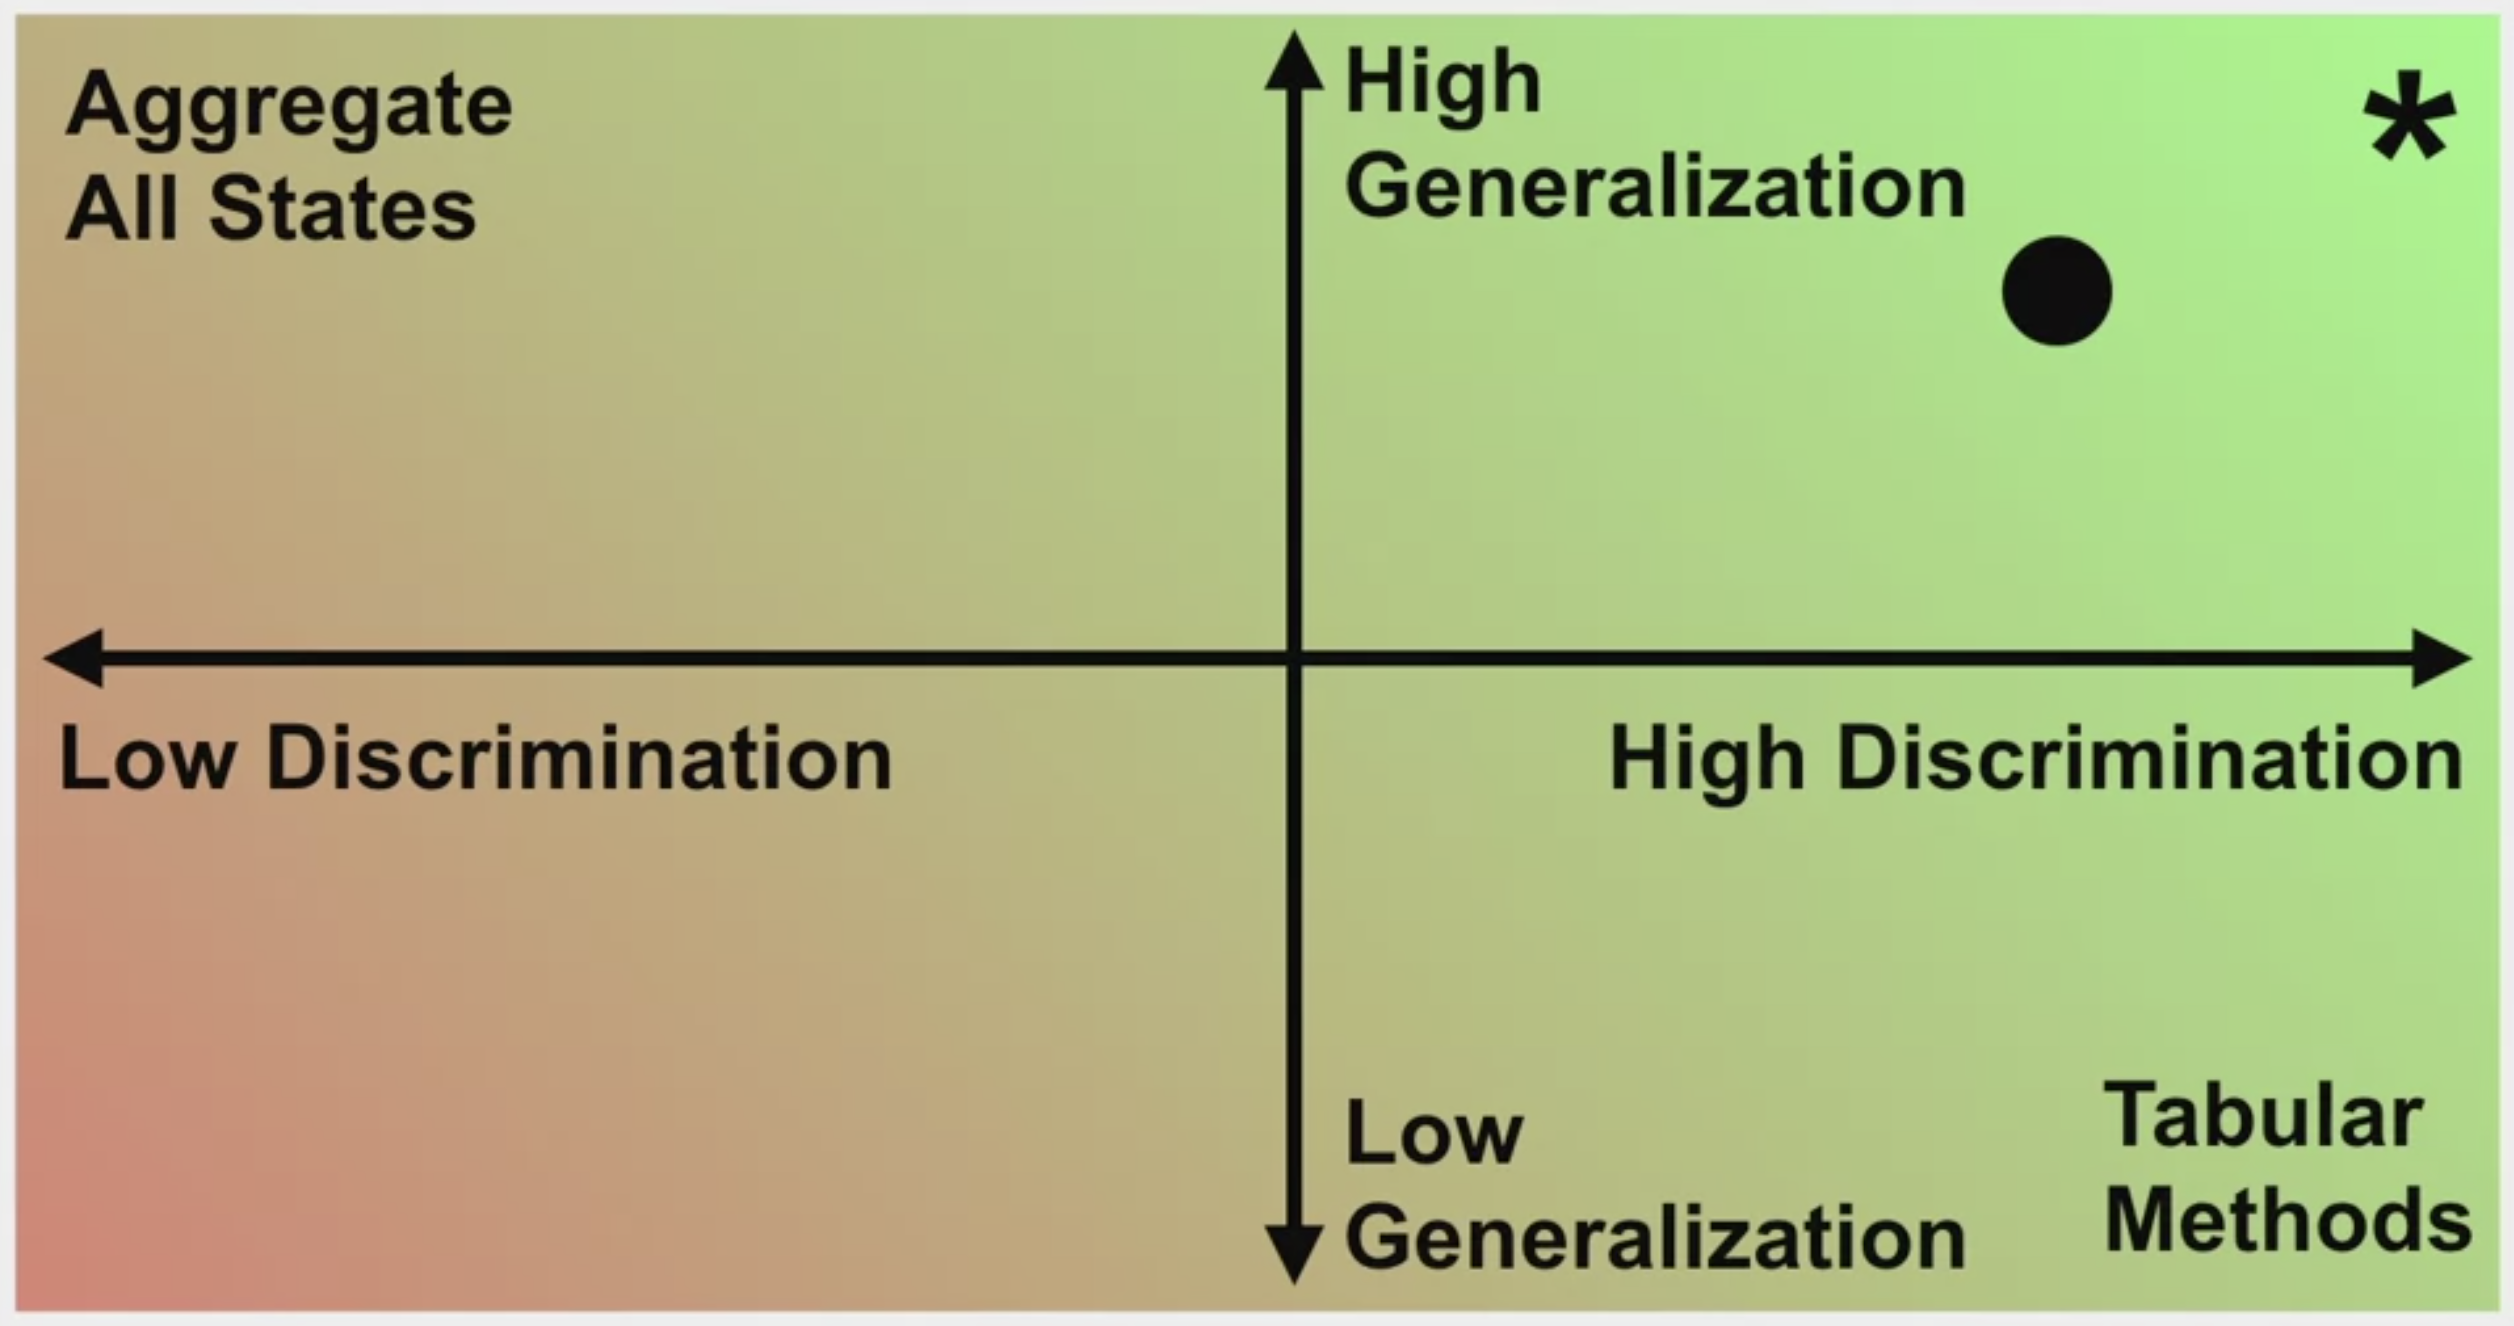
\includegraphics[width=0.8\columnwidth]{images/generalization-discrimination.png}
    \caption{Categorizing methods based on \textcolor{blue}{generalization} and \textcolor{blue}{discrimination}}
    \label{fig:generalization-discrimination}
\end{figure}
\begin{itemize}
  \item[*] = What we would really like is a learning method that achieves good generalization and a good discrimination. Such a method would generalize the learn values to similar states, allowing it to learn faster, but it could also discriminate between states. Meaning, with more data, the value function approximation can accurately represent the values.
  \item = In practice, we are more likely to get a point here, where we trade off some level of discrimination for generalization.
\end{itemize}

















\subsection{Prediction Objective $(\overline{VE})$}\label{prediction-objective}


Policy evaluation under \textit{function approximation} \textbf{requires us to specify an objective} $\rightarrow$ \textcolor{blue}{Mean Squared Value Error $(\overline{VE})$}:

$$
\overline{VE}(w) \doteq \sum_{s \in \mathcal{S}} \mu(s) (v_\pi(s) - \hat{v}(s, w))^2
$$


\textbf{Intuition:}
\begin{itemize}
  \item By assumption we have far \uline{more \textbf{states} than \textbf{weights}}, so \textcolor{Green}{making one state’s estimate more accurate} \textcolor{red}{invariably means making others' less accurate}.
  \item  We are \textcolor{Orange}{obligated then to say which states we care most about} $\rightarrow$ We must specify a \textbf{\textcolor{blue}{state distribution $\mu(s) > 0, \sum_s mu(s) = 1$}}, representing how much we care about the error in each state $s$. The \uline{states that the policy spends more time in have a higher weight in the objective}. We care less about errors in the states the policy visits less frequently.
\end{itemize}











\subsection{Stochastic-gradient and Semi-gradient Methods (for $\overline{VE}$ minimization)}\label{gradient-descent}


\subsubsection{Stochastic-gradient Methods}\label{stochastic-gradient-methods}


\textbf{Recall \textcolor{blue}{Derivative}:} tells us how to locally change $W$ to increase or decrease $f$.

\begin{figure}[H]
  \centering
    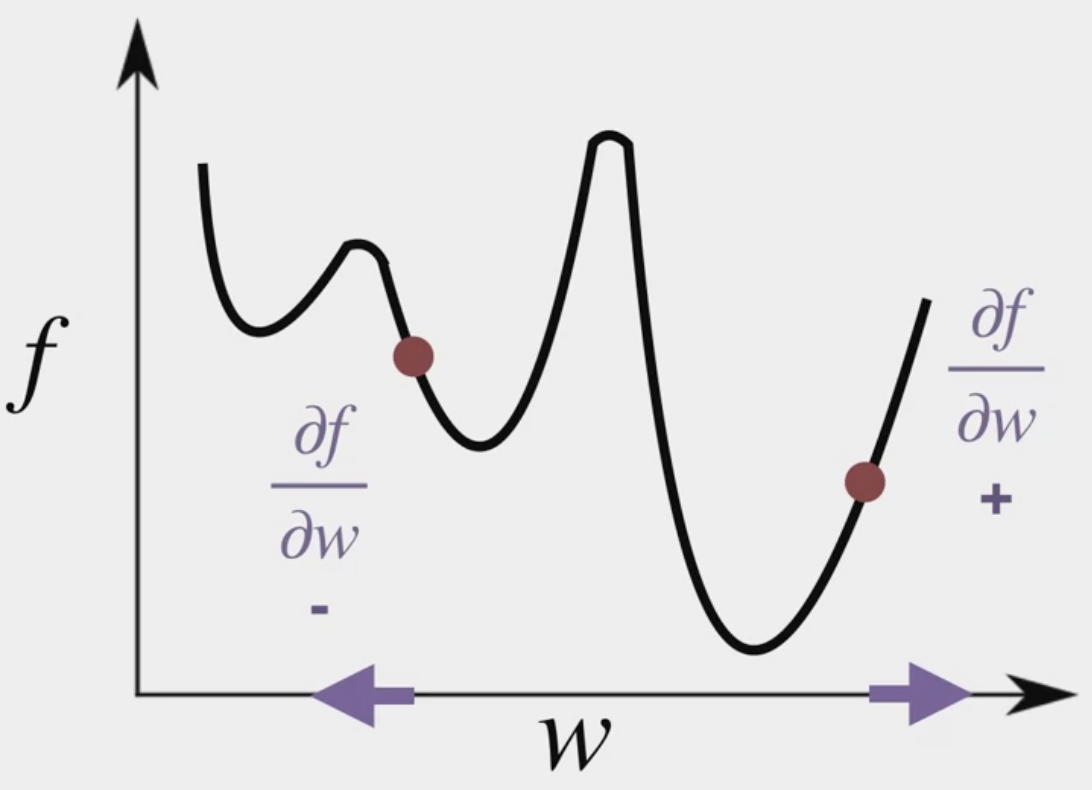
\includegraphics[width=0.8\columnwidth]{images/derivatives.png}
    \label{fig:derivatives}
\end{figure}

\begin{itemize}
  \item \textbf{Sign ($+ / -$):} indicates the direction to change $W$ to increase $f$.
  \item \textbf{Magnitude:} the slope of the function $f$ at the point $W$.
\end{itemize}

\textbf{\textcolor{blue}{Gradient}:} \textcolor{blue}{Derivative} on Multiple Dimensions. So it tells us how $f$ changes as the vector $W$ changes.
\begin{itemize}
  \item If $f$ is privatized by more than one variable, then $W$ is a vector. The gradient is a vector of partial derivatives, indicating how a local change in each component of $W$ affects the function $f$.
  $$
  w \doteq \begin{bmatrix}
                  w_{1} \\
                  w_{2} \\
                  ... \\
                  w_{d}
            \end{bmatrix} \;\;\;
  \nabla f \doteq \begin{bmatrix}
                  \frac{\partial f}{\partial w_{1}} \\
                  \frac{\partial f}{\partial w_{2}} \\
                  ... \\
                  \frac{\partial f}{\partial w_{d}}
                  \end{bmatrix}
  $$
  \begin{itemize}
    \item The sign of each component of the gradient specifies the direction to change the associated component of $W$, in order to increase $f$. The magnitude of the component specifies how quickly $f$ changes, as $W$ moves in that direction.
    \item The gradient \textcolor{Green}{\uline{gives the direction of steepest descent}. It provides the direction to change $W$, so that locally $f$ is maximally increased}.
  \end{itemize}
\end{itemize}



Mean Squared Value Error $(\overline{VE}(w))$ is a function of the weights to minimize with \textbf{\textcolor{blue}{Gradient Descent} (used to find stationary points of objectives)}.
\begin{itemize}
  \item Gradient Descent update rule:
  $$
  w_{t+1} \doteq w_t - \underbrace{\alpha}_\text{Step-Size} \underbrace{\nabla f(w_t)}_\text{Gradient}
  $$
  \begin{figure}[H]
    \centering
      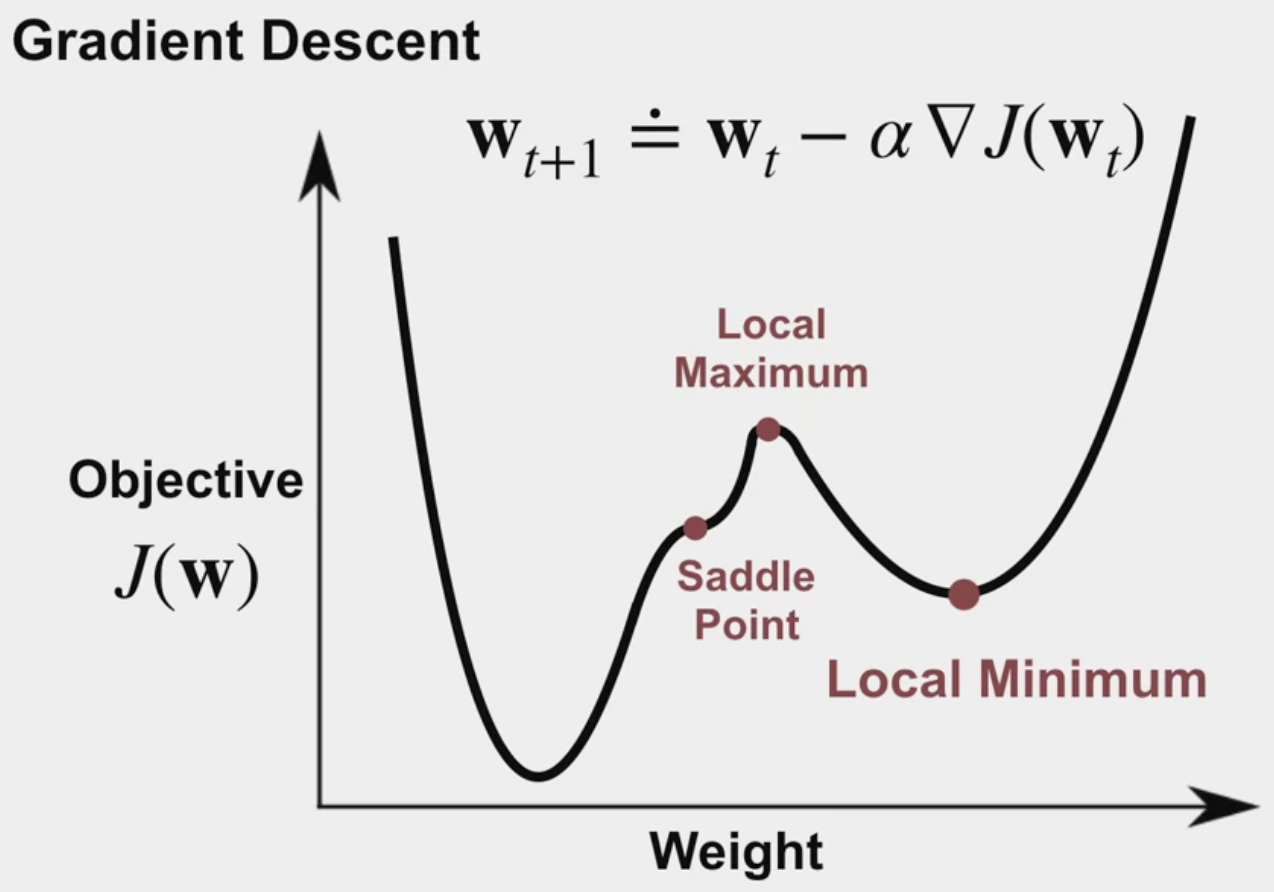
\includegraphics[width=0.8\columnwidth]{images/gradient-descent.png}
      \label{fig:gradient-descent}
  \end{figure}
  \begin{itemize}
    \item Local minima is stable, so gradient descent will tend to converge there. However, for convex functions, gradient descent is guaranteed to converge to the global minimum, which is the best possible setting of the weights for the objective.
  \end{itemize}
\end{itemize}






\textbf{\textcolor{blue}{Gradient} for Policy Evaluation:}

\begin{itemize}

  \item \textbf{\textcolor{red}{(Standard) Gradient Descent:}}
  \begin{figure}[H]
    \centering
      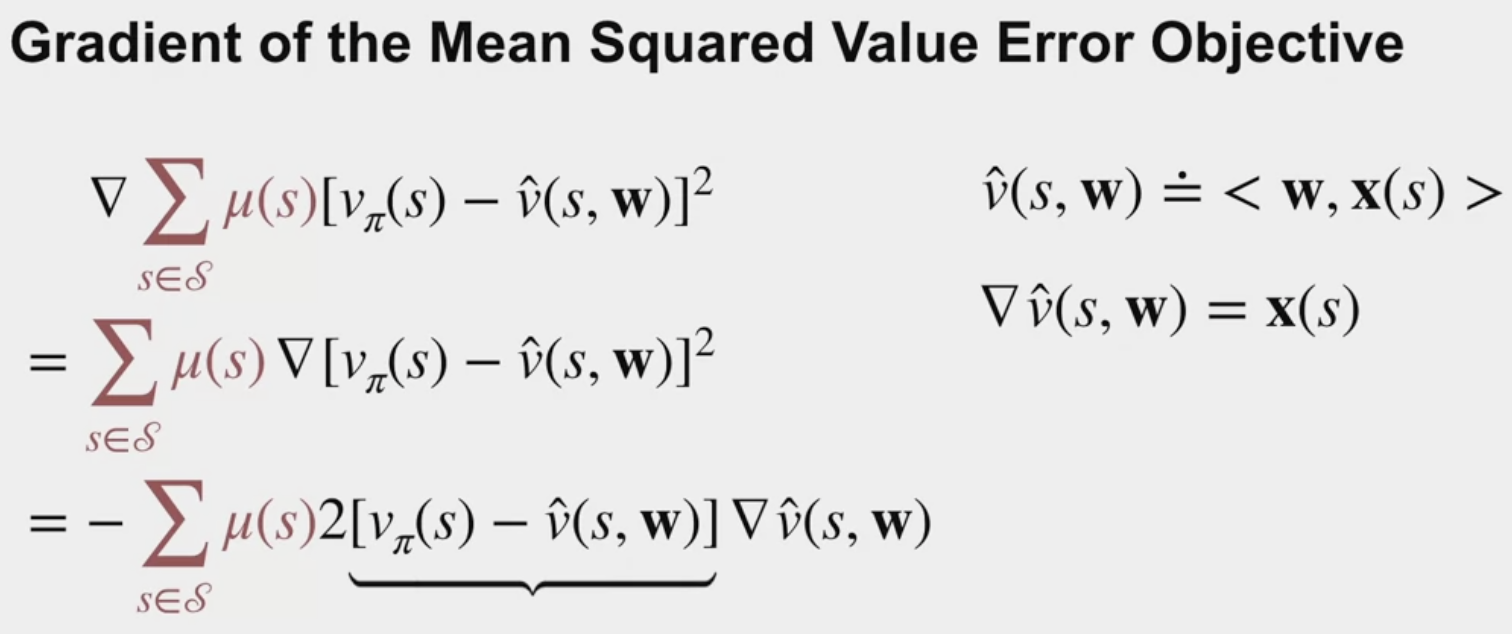
\includegraphics[width=0.8\columnwidth]{images/gradient-for-mse.png}
      \label{fig:gradient-for-mse}
  \end{figure}

  \begin{itemize}
    \item The gradient of the value function approximation indicates how to change the weights to increase the value for that state.
    \item Computing the gradient for $\overline{VE}$ \textcolor{Orange}{requires summing over all states}. This is generally \textcolor{red}{not feasible for large state spaces}. Also, we likely \textcolor{red}{do not know the distribution $\mu$}.
  \end{itemize}

  \item \textbf{\textcolor{Orange}{Stochastic Gradient Descent:} only uses a stochastic estimate of the gradient (to approximate this gradient).}

  \begin{itemize}
    \item[]
    \begin{itemize}
      \item expectation of each stochastic gradient = gradient of the objective
    \end{itemize}

    \item Though \textcolor{Orange}{we do not explicitly have $\mu$}, we can \textcolor{Green}{sample states from it simply by following the policy}. We can use the $(S, v_\pi(S))$ pairs to make an update to decrease the error on states.
    \item \textbf{By making small updates in the direction that improves error on each $(S, v_\pi(S))$ pair}, we \textcolor{Orange}{might sometimes increase the error on the full objective}. But the \textcolor{Green}{overall trend will be to make progress for the full objective}.
    \item \textcolor{red}{One remaining practical issue:} we \textcolor{red}{do not have access to $v_\pi$}.

  \end{itemize}

  \item \textbf{\textcolor{Green}{Gradient Monte Carlo} for value estimation:}

  \begin{itemize}
    \item We can get rid of $v_\pi$ from our update rule.
    \item Using samples of the return for each visited state, $S_t$, as we did for Monte Carlo methods.
    \begin{figure}[H]
      \centering
        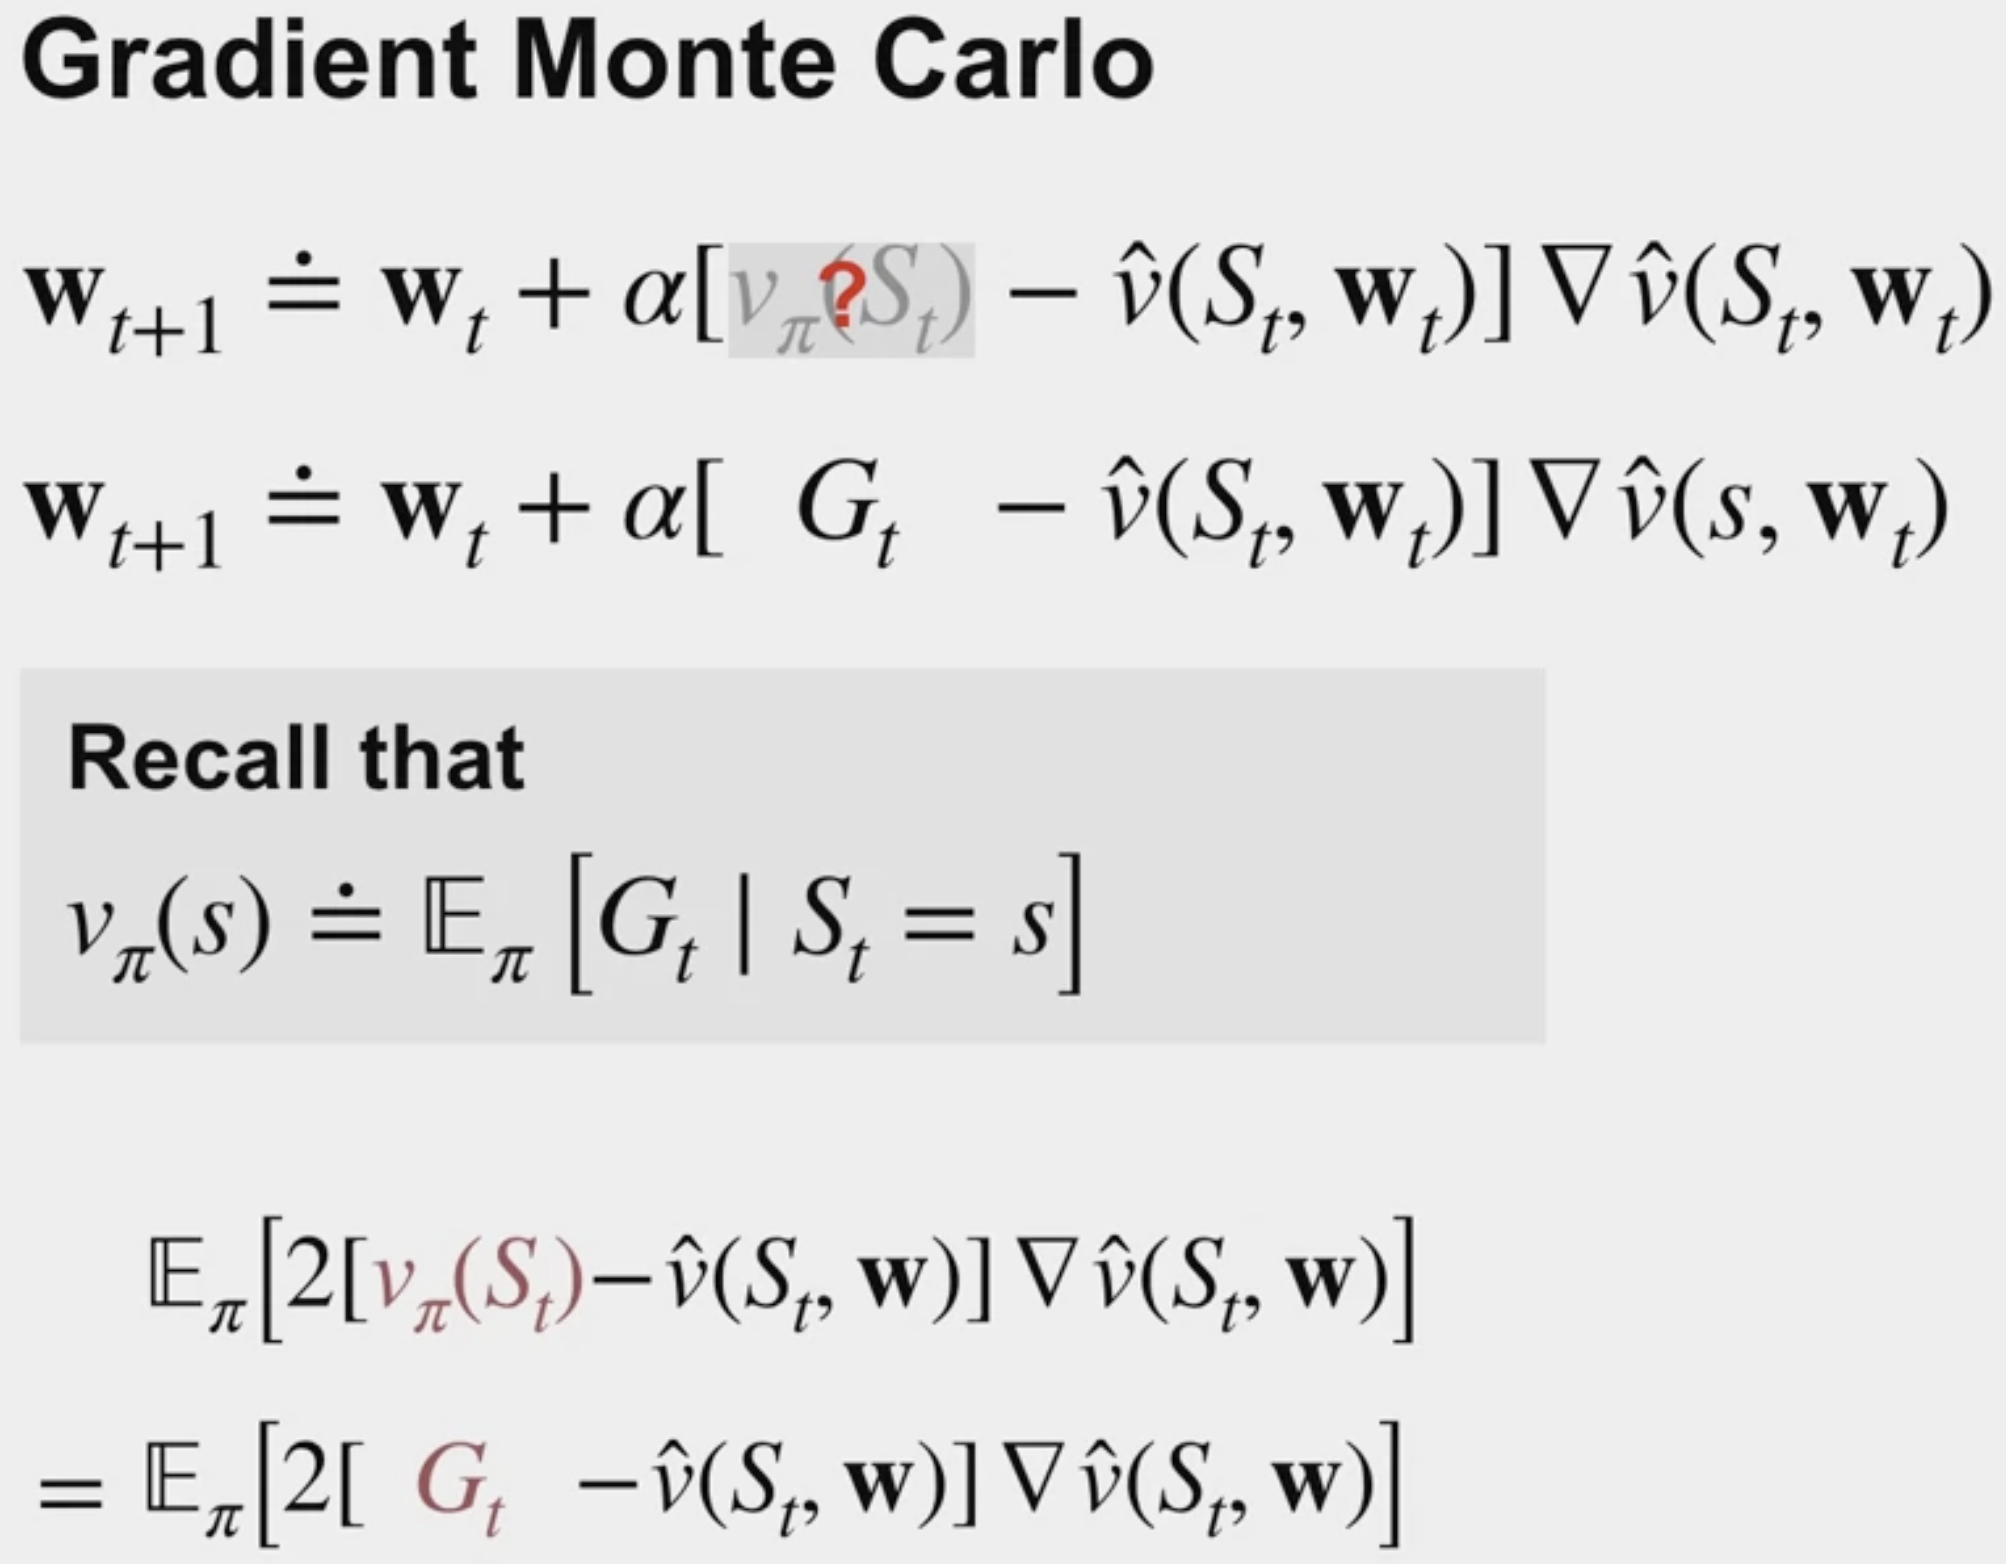
\includegraphics[width=0.6\columnwidth]{images/gradient-monte-carlo.png}
        \label{fig:gradient-monte-carlo}
    \end{figure}
  \end{itemize}

\end{itemize}




\begin{tcolorbox}[title={Gradient Monte Carlo Algorithm for Estimating $\hat{v} \approx v_\pi$}]

  \textbf{Input:} the policy $\pi$ to be evaluated

  \textbf{Input:} a differentiable function $\hat{v}: \mathcal{S} \times \mathbb{R}^d \to R$

  \textbf{Algorithm parameter:} step size $\alpha > 0$

  \textbf{Initialize:} value-function weights $w \in \mathbb{R}^d$ arbitrarily (e.g., $w=0$)

  \textbf{Loop forever (for each episode):}
  \begin{description}
      \item $\;\;\;$ Generate an episode using $\pi$
      \item $\;\;\;$ \textbf{Loop for each step of episode, $t=0,1,...,T-1$:}
      \begin{description}
        \item $\;\;\;$ $w \leftarrow w + \alpha (G_t -\hat{v}(S_t, w)) \nabla \hat{v}(S_t, w)$
      \end{description}
  \end{description}
\end{tcolorbox}


\bigskip

\textbf{Example:} Gradient Monte Carlo with State Aggregation
\begin{itemize}
  \item Random walk starting from 500, terminating in either 0 (w. return -1) or 1 (w. return +1).
  \item With state aggregation, aggregate the 1000 states to 10 weights.
  \begin{figure}[H]
    \centering
      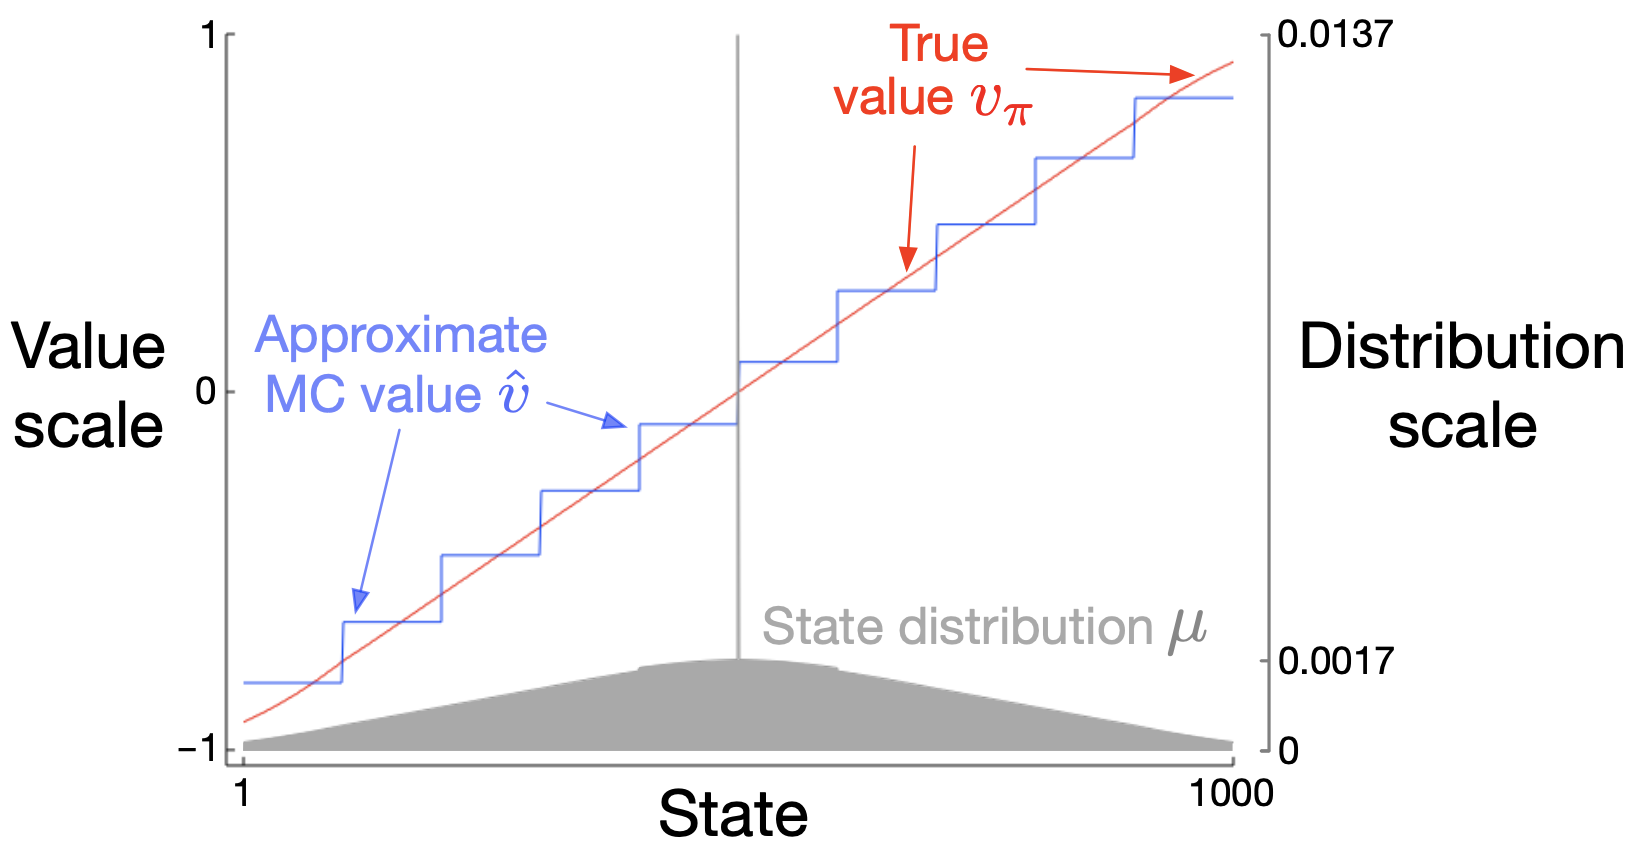
\includegraphics[width=0.8\columnwidth]{images/gradient-monte-carlo-with-state-aggregation.png}
      \label{fig:gradient-monte-carlo-with-state-aggregation}
  \end{figure}
\end{itemize}






\subsubsection{Semi-gradient TD}\label{semi-gradient-td}

\textbf{What:} TD learning with function approximation (approximation to stochastic gradient descent).

\begin{itemize}
  \item \textit{Semi-gradient method}, as TD is not performing gradient descent updates on the squared error. It's not a gradient descent algorithm.
\end{itemize}


\begin{tcolorbox}[title={Semi-gradient TD(0) for estimating $\hat{v} \approx v_\pi$}]

  \textbf{Input:} the policy $\pi$ to be evaluated

  \textbf{Input:} a differentiable function $\hat{v}: \mathcal{S}^+ \times \mathbb{R}^d \to R$ such that $\hat{v}(terminal,\cdot) = 0$

  \textbf{Algorithm parameter:} step size $\alpha > 0$

  \textbf{Initialize:} value-function weights $w \in \mathbb{R}^d$ arbitrarily (e.g., $w=0$)

  \textbf{Loop for each episode:}
  \begin{description}
      \item $\;\;\;$ Initialize $S$
      \item $\;\;\;$ \textbf{Loop for each step of episode:}
      \begin{description}
        \item $\;\;\;$ Choose $A \sim \pi(\cdot | S)$
        \item $\;\;\;$ Take action $A$, observe $R, S'$
        \item $\;\;\;$ $w \leftarrow w + \alpha ((R + \gamma \hat{v}(S',w)) -\hat{v}(S, w)) \nabla \hat{v}(S, w)$
        \item $\;\;\;$ $S \leftarrow S'$
      \end{description}
      \item $\;\;\;$ \textbf{Until $S$ is terminal}
  \end{description}
\end{tcolorbox}


We can denote approximation of $v_\pi(S_t)$ with $U_t$. This yields the following \textcolor{blue}{general SGD update} for state-value prediction:

$$
w_{t+1} \doteq w_t + \alpha (U_t - \hat{v}(S_t,w_t)) \nabla \hat{v}(S_t, w_t)
$$



\textbf{\textcolor{blue}{Semi-gradient TD} vs \textcolor{blue}{Gradient Monte Carlo}:}
\begin{itemize}
  \item \textbf{\textcolor{blue}{Semi-gradient TD}:} biased TD updates $\rightarrow$ \textcolor{red}{cannot guarantee convergence to a local minimum}. But we often prefer TD learning over Monte Carlo anyway because it can \textcolor{Green}{converge more quickly}, due to taking advantage of bootstrapping.
  \item \textbf{\textcolor{blue}{Gradient Monte Carlo}:} \textcolor{Green}{converge to a local minimum}
\end{itemize}










\subsection{Linear Methods}\label{linear-methods}

\textbf{What:} Linear value function approximation is a strict generalization of tabular value function approximation.


\textbf{Benefits:}
\begin{itemize}
  \item Linear methods are \textcolor{Green}{simpler to understand} and analyze mathematically.
  \item Linear methods are interesting because of their \textcolor{Green}{convergence guarantees}, but also because in practice they \textcolor{Green}{can be very efficient in terms of both data and computation}.
  \item Much of the theory of TD learning is for the linear setting.
\end{itemize}


\textbf{Linear methods} approximate the state-value function by the inner product between $w$ and $x(s)$:
\begin{gather*}
  \hat{v}(s,w) \doteq w^T x(s) \doteq \sum_{i=1}^d w_i x_i (s) \\ \\
  \textbf{Where:} \\
  x(s) \text{: \textit{feature vector} representing state $s$}
\end{gather*}

It is natural to use Stochastic Gradient Descent (SGD) updates with linear function approximation. The \uline{\textbf{gradient} of the approximate value function with respect to $w$} in this case is
$$
\nabla \hat{v}(s,w) = x(s)
$$

Thus, in the linear case the \textcolor{blue}{general SGD update} reduces to a particularly simple form:

$$
w_{t+1} \doteq w_t + \alpha (U_t - \hat{v}(S_t,w_t)) x(S_t)
$$



\textbf{\textcolor{blue}{Linear (Semi-gradient) TD}}
\begin{itemize}
  \item \textbf{Converges} to a well understood approximation called the \textcolor{blue}{TD fixed point $W_{TD}$}.
  \begin{itemize}
    \item It is a solution to this linear system:
    $$
    \textcolor{blue}{W_{TD}} = A^{-1} b
    $$
    \item Converged when (\textcolor{purple}{Expected TD Update $= 0$})
  \end{itemize}
  \item TD update with linear function approximation: \textcolor{purple}{Expected TD Update}. It characterizes the \uline{expected change in the weight from one time step to the next}.
  $$
  \mathbb{E}[ \Delta \textcolor{blue}{W_{TD}}] = w_t + \alpha (b - A \textcolor{blue}{W_{TD}})
  $$
  \begin{itemize}
    \item \textbf{Where:}
    \begin{itemize}
      \item \textbf{matrix $A$} is defined in terms of an \uline{expectation over the features}
      $$
      A \doteq \mathbb{E}[x_t (x_t - \gamma x_{t+1})^T]
      $$
      \item \textbf{vector $b$} vector b is defined in terms of the \uline{reward and the features}
      $$
      b \doteq \mathbb{E}[R_{t+1} x_t]
      $$
    \end{itemize}
  \end{itemize}
  \item \textbf{Key takeaway} is that even though TD does not converge to the minimum of the mean squared value error, It does \uline{converge to the minimum of a principled objective, based on Bellman equations}.
\end{itemize}












\subsection{Feature Construction for Linear Methods}\label{feature-construction-for-linear-methods}

Here we discuss different ways to construct state, and state-action features.

\textbf{Choosing features appropriate to the task} is an \uline{important way of adding prior domain knowledge} to reinforcement learning systems.

A \textbf{limitation of the linear} form is that it \textcolor{red}{cannot take into account any interactions between features}, such as the presence of feature i being good only in the absence of feature j.





\subsubsection{Polynomials}\label{polynomials}

While the basic polynomial features we discuss here \textcolor{red}{do not work as well as other types of features in RL}, they serve as a good introduction because they are simple and familiar.




\subsubsection{Fourier Basis}\label{fourier-basis}

Another linear function approximation method is based on the time-honored Fourier series, which \uline{expresses periodic functions as weighted sums of sine and cosine basis functions (features) of different frequencies}.

In RL, where the functions to be approximated are unknown, Fourier basis functions are of interest because they are \textcolor{Green}{easy to use and can perform well in a range of RL problems}.



\subsubsection{Coarse Coding}\label{coarse-coding}

Recall, \textbf{state aggregation:} is the process of aggregating states for a smaller number of weights. Similar states are aggregated together.

\begin{itemize}
  \item \textbf{Example:} represent the location of this fish that's swimming in a pond, a two-dimensional continuous state space:
  \begin{figure}[H]
    \centering
      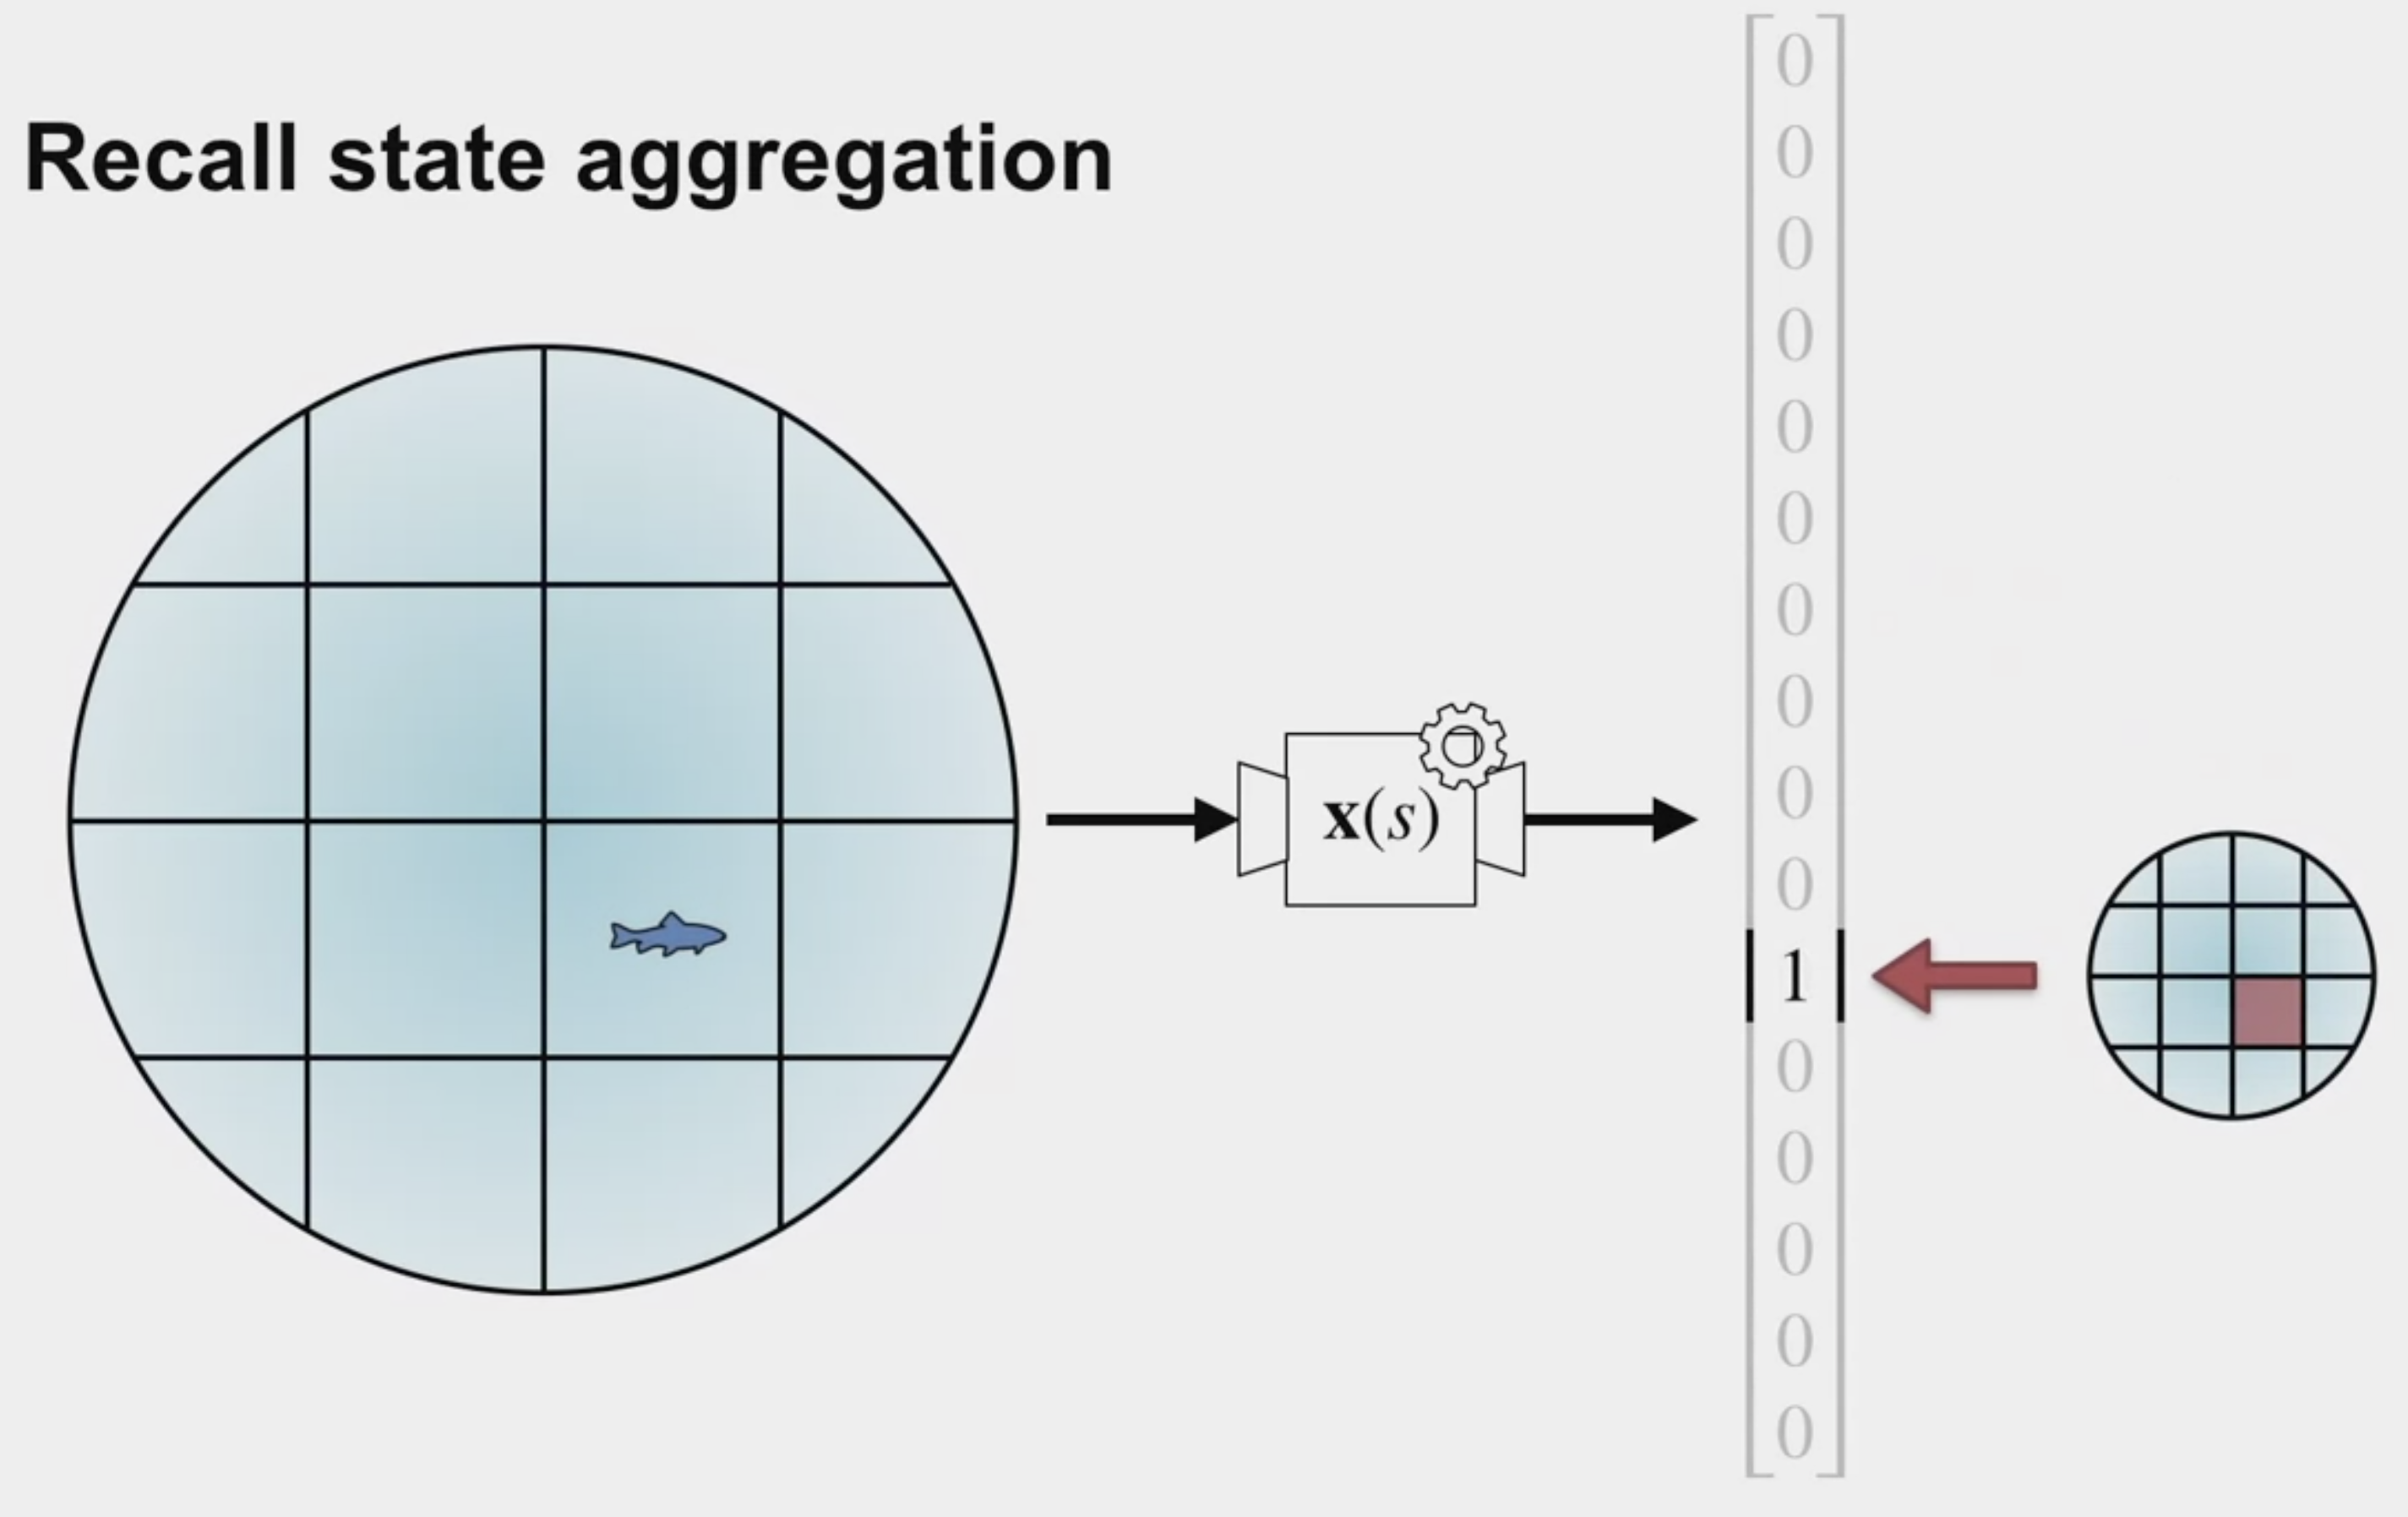
\includegraphics[width=0.7\columnwidth]{images/state-aggregation-eg.png}
      \label{fig:state-aggregation-eg}
  \end{figure}
\end{itemize}



\textbf{\textcolor{blue}{Course coding}} is a generalization of state aggregation that allows shapes to overlap. By allowing the shapes to overlap, we obtain a more \uline{flexible class of \textbf{feature representations}} called course coding.

\begin{itemize}
  \item \textbf{Example:} represent the location of this fish that's swimming in a pond, a two-dimensional continuous state space:
  \begin{figure}[H]
    \centering
      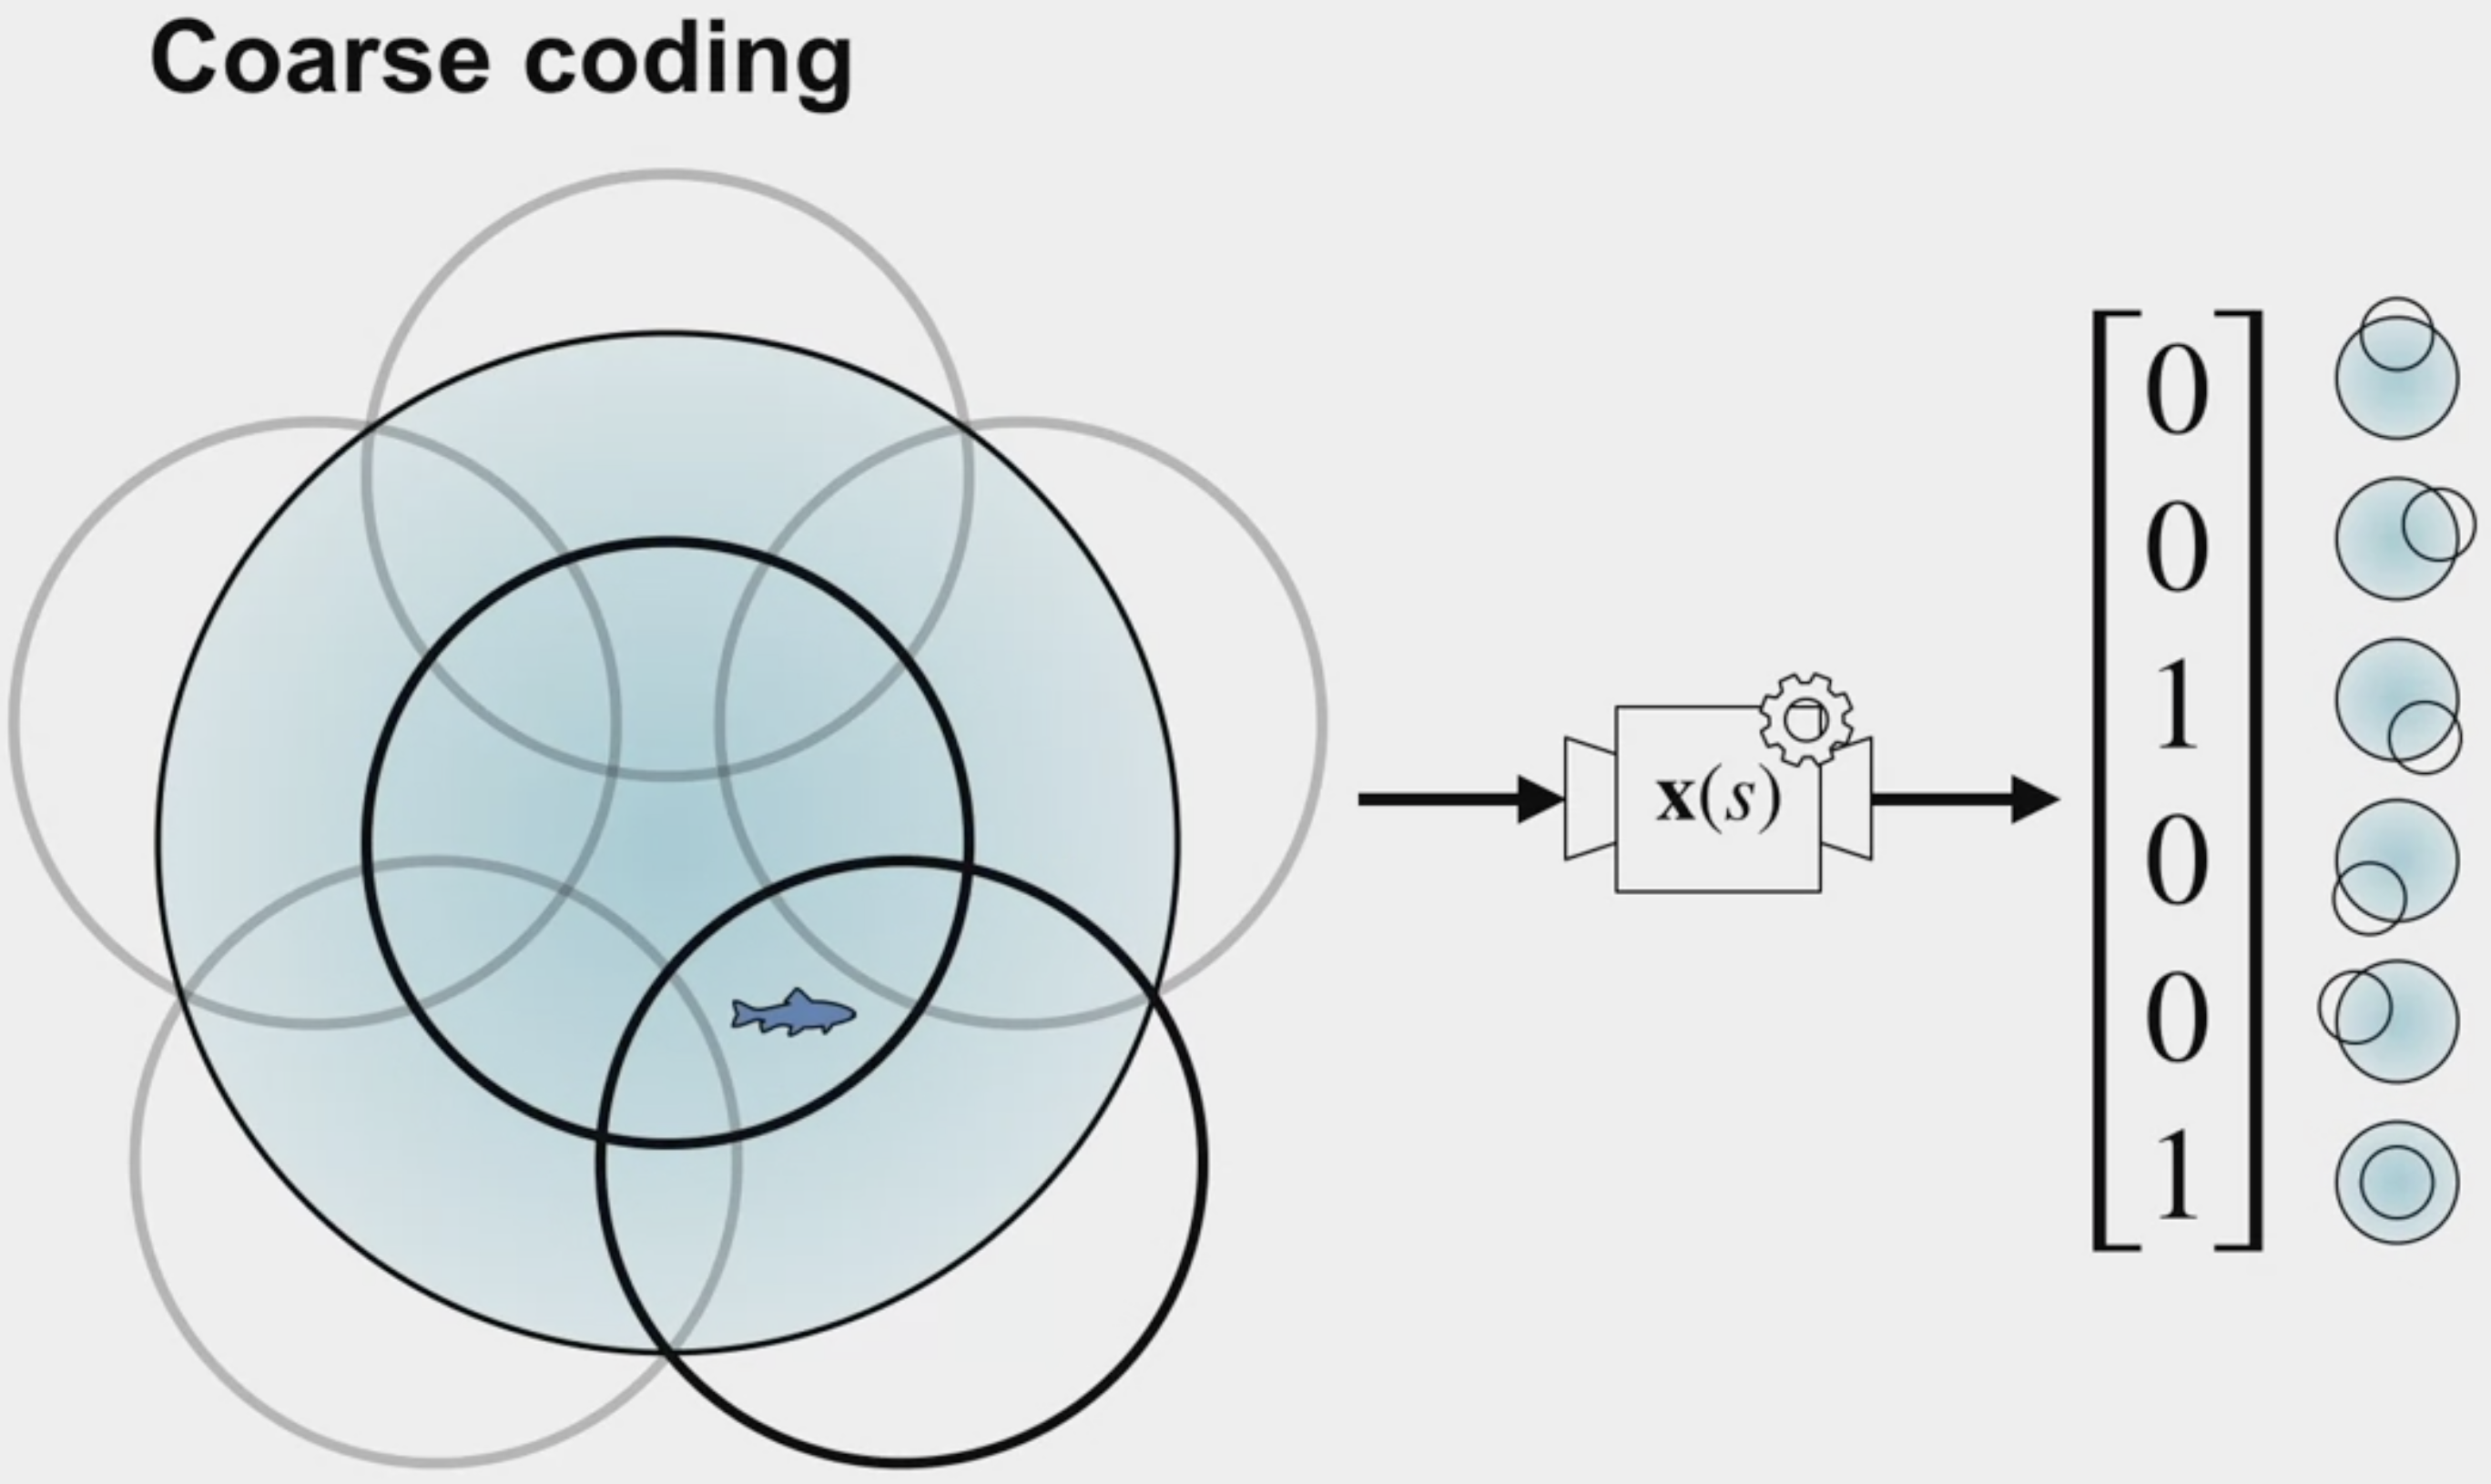
\includegraphics[width=0.7\columnwidth]{images/coarse-coding-eg.png}
      \label{fig:coarse-coding-eg}
  \end{figure}
\end{itemize}


\textbf{Generalization Properties of Coarse Coding:}
\begin{itemize}
  \item If the union of the receptive fields for the active features is large, the feature representation generalizes more.
  \item Using different shapes in coarse coding can change the direction of generalization as well.
  \item The overlap between shapes dictates the level of discrimination.
  \item Every state within the same shape will have the exact same feature vector. As a result, they must all have the same approximate value.
  \item \uline{size, number, and shape of the features} all affect the \textbf{discriminative ability} of the representation.
\end{itemize}





\subsubsection{Tile Coding}\label{tile-coding}

\textbf{What:} a \textcolor{Green}{computationally efficient} way to perform \uline{Course Coding}.

\textbf{How:} performs an exhaustive \uline{partition of the state space using overlapping grids} $\rightarrow$ many small intersections $\rightarrow$ better discrimination.

\begin{itemize}
  \item Put several tilings on top of each other, with each tiling is offset by a small amount.
  \item For:
  \begin{itemize}
    \item \textbf{one tiling}, generalization only occurs within the square
    \item \textbf{multiple tilings}, updates in a state generalize to other intersecting states
  \end{itemize}
\end{itemize}

layering squares over this squished environment is like laying rectangles over the unsquished environment. By using rectangles, we can control the broadness of the generalization across each dimension of the state-space.


Good in low dimensional environments. However, \textcolor{red}{as the number of dimensions grows, the number of required tiles grows exponentially}. As a result, it can be necessary to tile input dimension separately.

\begin{itemize}
  \item \textbf{Example:} represent the location of this fish that's swimming in a pond, a two-dimensional continuous state space:
  \begin{figure}[H]
    \centering
      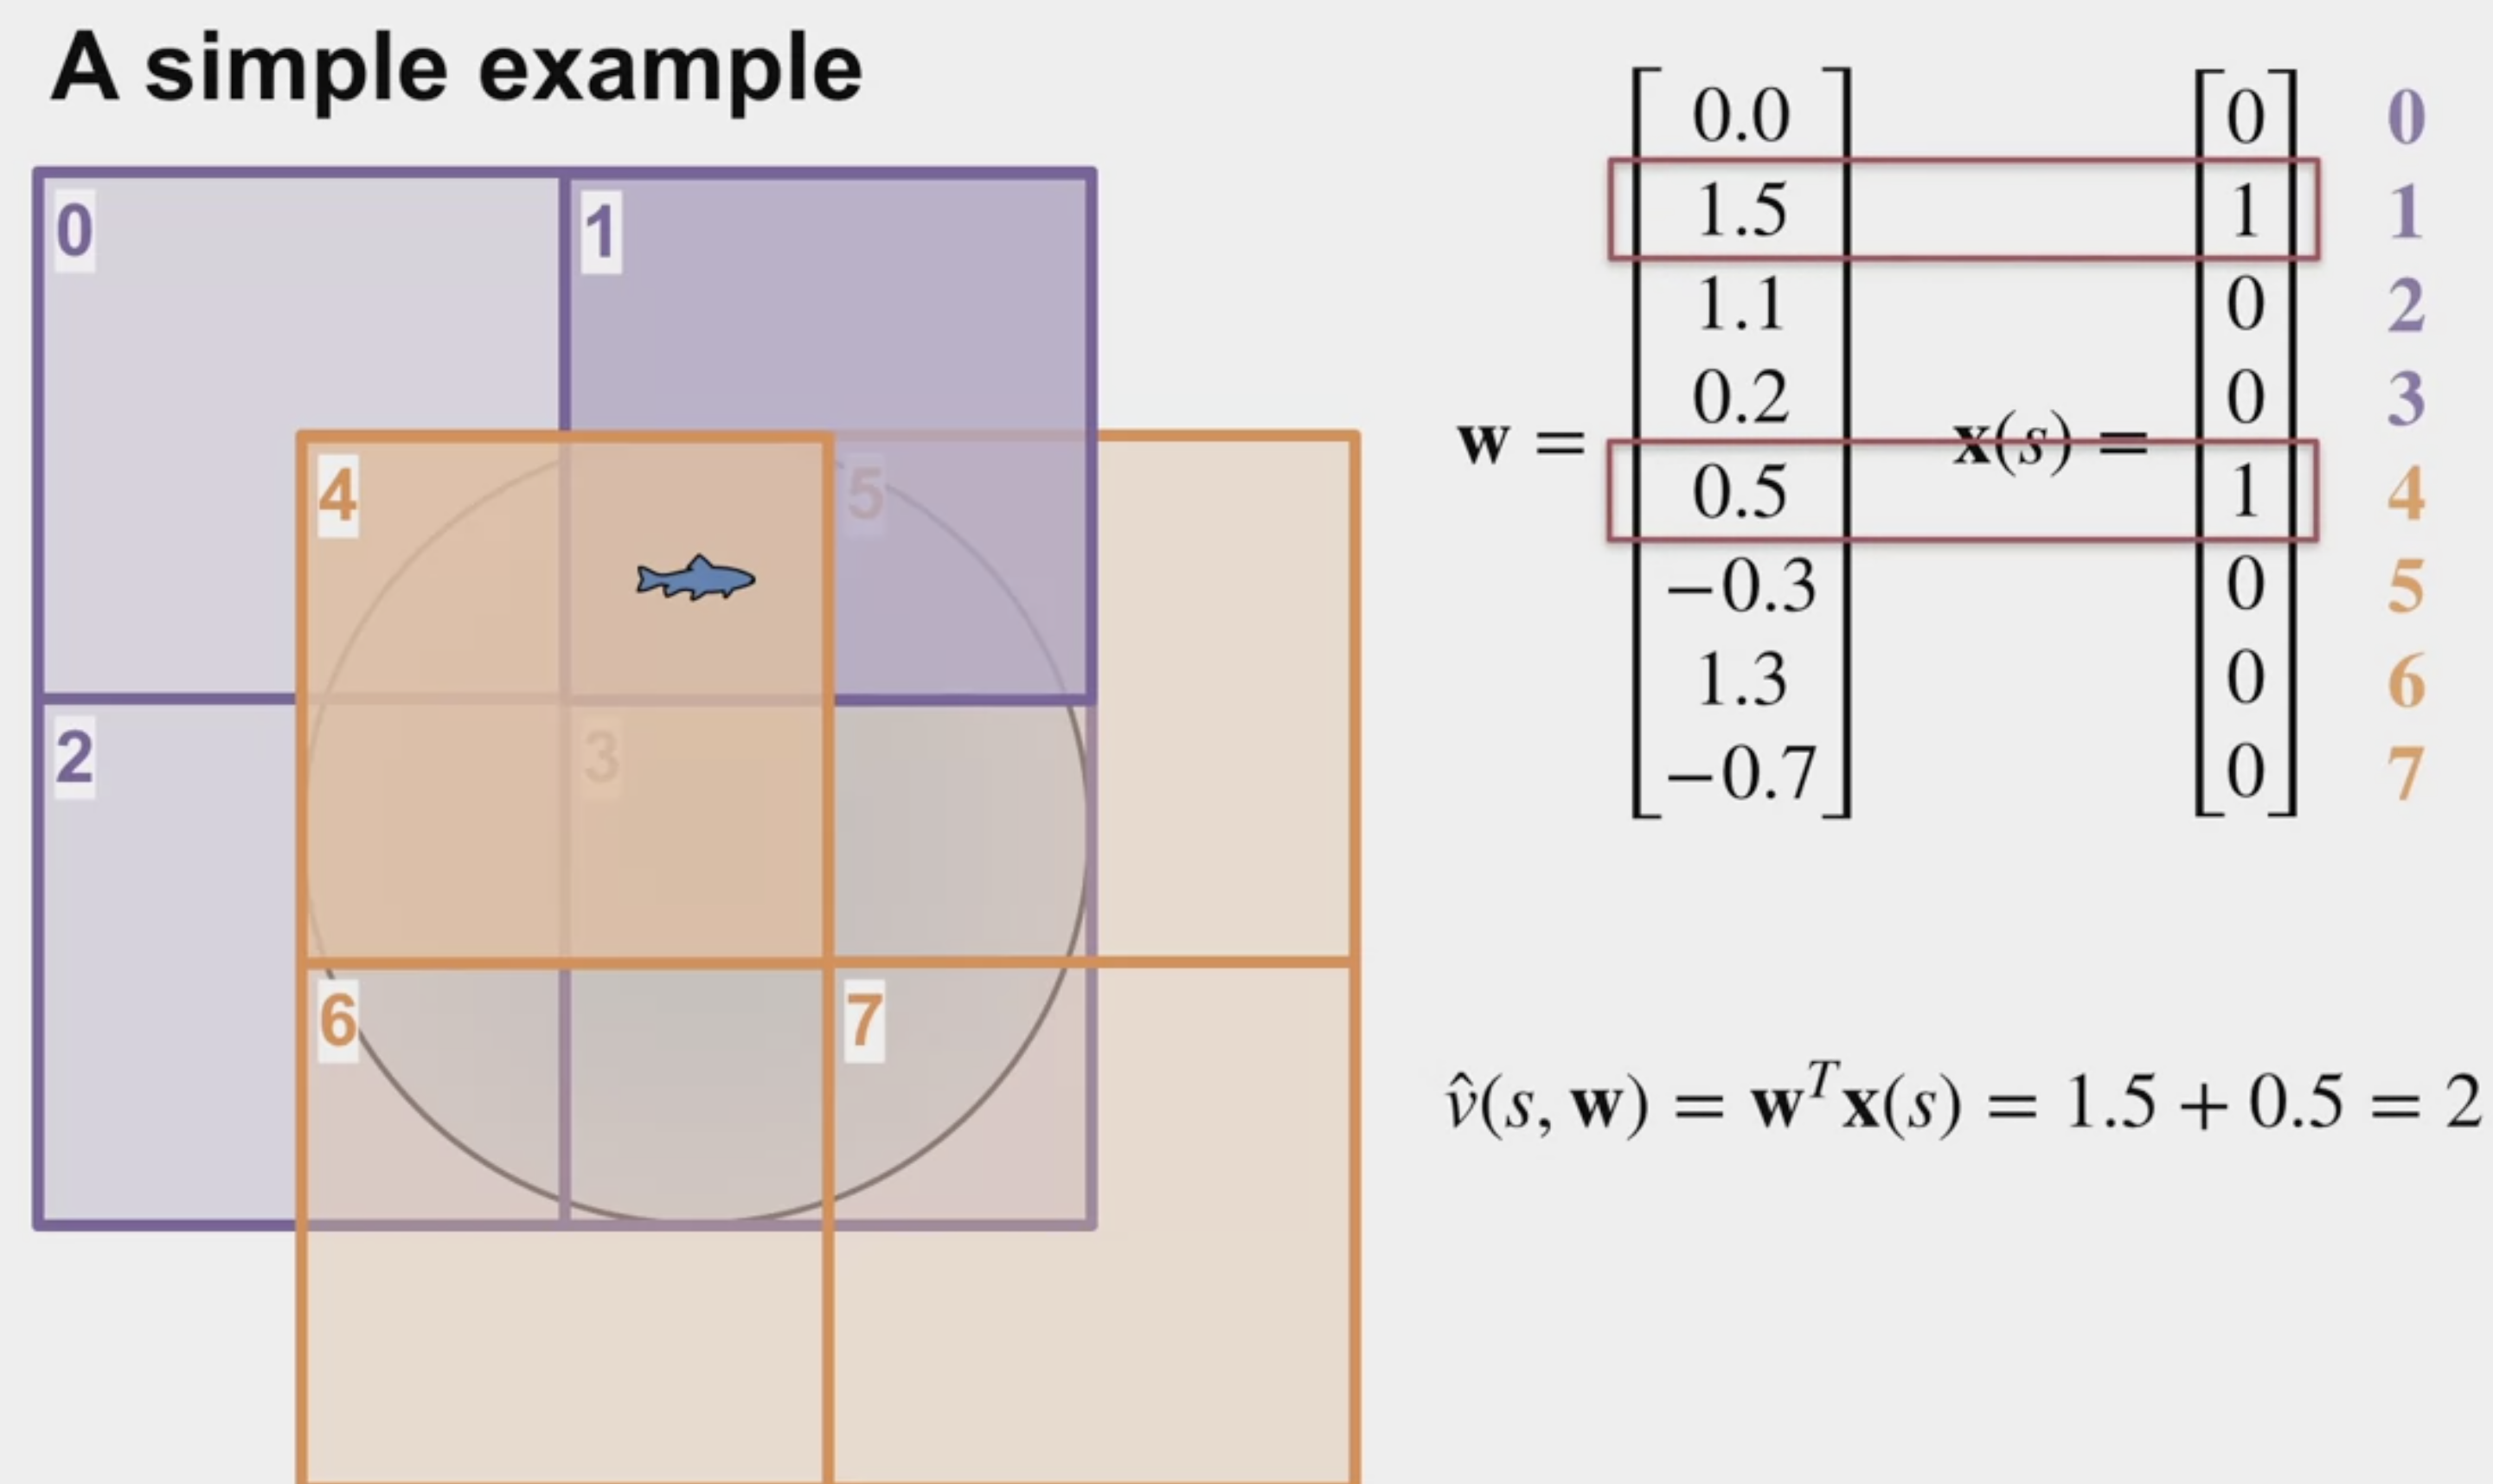
\includegraphics[width=0.7\columnwidth]{images/tile-coding-eg.png}
      \label{fig:tile-coding-eg}
  \end{figure}
\end{itemize}














\subsubsection{Radial Basis Functions (RBFs)}\label{radial-basis-functions}

\textbf{What:} natural generalization of coarse coding to continuous-valued features.


\textbf{How:} Rather than each \textbf{feature} being either 0 or 1, it \uline{can be anything in the interval [0, 1]}, reflecting various \textit{degrees} to which the feature is present.

A \textbf{typical RBF feature}, $x_i$, has a Gaussian (bell-shaped) response $x_i(s)$ dependent only on the distance between the state, $s$, and the feature’s prototypical or center state, $c_i$, and relative to the feature’s width, $\sigma_i$:

$$
x_i(s) \doteq \exp{\left(-\frac{||s-c_i||^2}{2\sigma_i^2}\right)}
$$

The \textbf{norm} or \textbf{distance metric} of course can be chosen in whatever way seems most appropriate to the states and task at hand. The figure below shows a one-dimensional example with a Euclidean distance metric.

\begin{figure}[H]
  \centering
    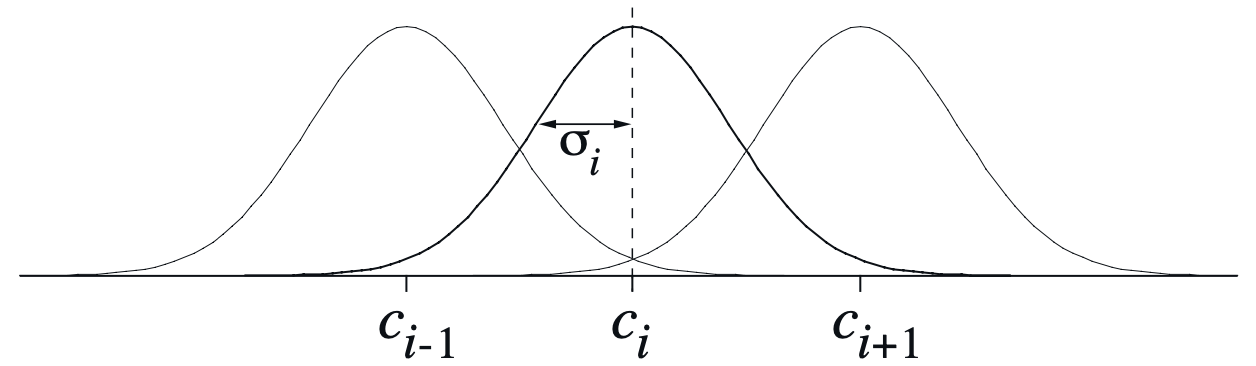
\includegraphics[width=0.7\columnwidth]{images/radial-basis-functions.png}
    \caption{One-dimensional radial basis functions.}
    \label{fig:radial-basis-functions}
\end{figure}


The primary advantage of RBFs over binary features is that they produce \textcolor{Green}{approximate functions that vary smoothly and are differentiable}. Although this is appealing, \textcolor{red}{in most cases it has no practical significance}.











\subsection{Selecting Step-Size Parameters Manually}\label{selecting-stepsize-parameters-manually}

Most SGD methods require the designer to select an appropriate step-size parameter $\alpha$. Ideally selecting the step-size parameter $\alpha$ would be automated, and in some cases it has been, but for most cases it is still common practice to set it manually.

The classical choice:

$$
\alpha_t = 1/t
$$
\begin{itemize}
  \item produces sample averages in tabular MC methods
  \item \textcolor{red}{not appropriate for} \uline{TD methods}, for \uline{nonstationary problems}, or for \uline{any method using function approximation}.
\end{itemize}

In tabular case
\begin{itemize}
  \item $\alpha = 1$ will result in a complete elimination of the sample error after one target (we usually want to learn slower than this).
  \item a step size of $\alpha = \frac{1}{10}$ would take about 10 experiences to converge approximately to their mean target, and if we wanted to learn in 100 experiences we would use $\alpha = \frac{1}{100}$.
  \item In general, if $\alpha = \frac{1}{\tau}$, then the tabular estimate for a state will approach the mean of its targets, with the most recent targets having the greatest effect, after about $\tau$ experiences with the state.
\end{itemize}

With general function approximation there is not such a clear notion of number of experiences with a state, as each state may be similar to and dissimilar from all the others to various degrees. However, there is a similar rule that gives similar behavior in the case of linear function approximation. Suppose you wanted to learn in about $\tau$ experiences with substantially the same feature vector. A good rule of thumb for setting the step-size parameter of linear SGD methods is then

$$
\alpha \doteq (\tau \mathbb{E}[x^Tx])^{-1}
$$

where x is a random feature vector chosen from the same distribution as input vectors will be in the SGD. This method works best if the feature vectors do not vary greatly in length; ideally $x^Tx$ is a constant.










\subsection{Nonlinear Function Approximation: Artificial Neural Networks}\label{neural-networks}

\textbf{What:} a flexible and powerful class of nonlinear function approximators.

\textbf{Why:} Neural networks provide a strategy \textcolor{Green}{for learning a useful set of features}.

\textbf{Feed forward pass of a neural network mathematically (e.g.):}
\begin{figure}[H]
  \centering
    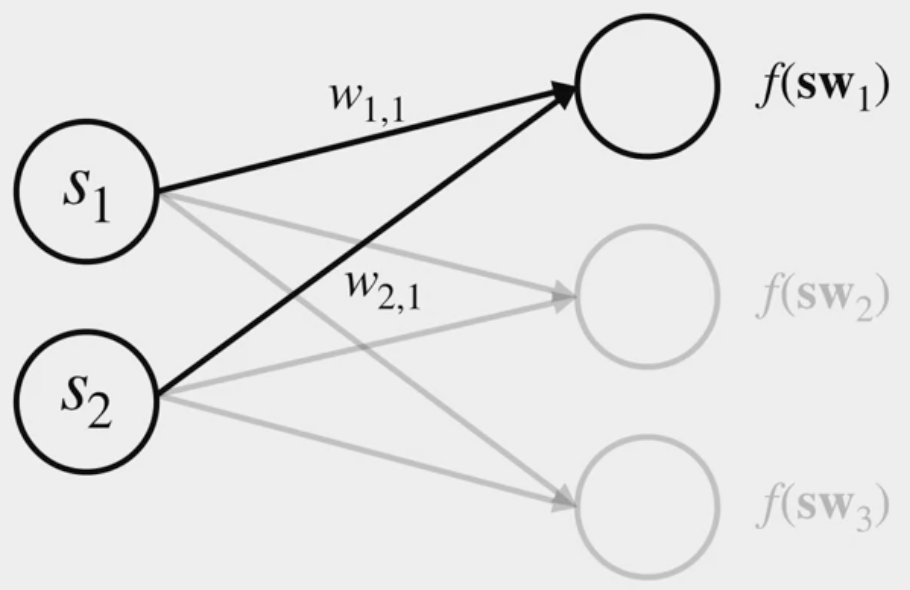
\includegraphics[width=0.7\columnwidth]{images/ann-feed-forward.png}
    \label{fig:ann-feed-forward}
\end{figure}
\begin{itemize}
  \item At \textbf{each node} we have \uline{two vectors}:
  \begin{itemize}
    \item Inputs: $s = [s_1, s_2]$
    \item Weights for each input: $w_1 = [w_{1,1}, w_{2,1}]^T$
  \end{itemize}
  \item At \textbf{each node} we \uline{dot product} the weights $w_1$ with the input $s$ and pass the result through the \uline{activation function} $f(s \times w_t)$.
  \item \textbf{Each node} has a \uline{different set of weights} $\rightarrow$ produce a \uline{different output}, (which we call a \textit{feature}).
\end{itemize}

So neural networks can be viewed as a \uline{way to construct features}, and that neural networks are \uline{non-linear functions of state}.


\textbf{Deep Neural Networks:}
\begin{itemize}
  \item \textbf{Why:} depth can \textcolor{Green}{facilitate learning features} \textbf{through} \uline{composition} and \uline{abstraction}.
  \item \textbf{Challenge:} In practice, \textcolor{Orange}{picking the right architecture can be difficult and can significantly impact performance}.
  \item \textbf{Universal Approximation Property:} in theory, a neural network need not be deep. A neural network with a \uline{single hidden layer can approximate any continuous function given that is sufficiently wide}.
  \item \textbf{Depth =} \# of hiddel layers in the network
  \begin{itemize}
    \item \textcolor{Green}{allows \uline{composition of features}} $\rightarrow$ \textcolor{Green}{can produce \uline{more specialized features} by combining modular components.}
    \item can also be \textcolor{Green}{helpful for obtaining abstractions}. Deep neural networks \uline{compose many layers of lower-level abstractions with each successive layer} contributing to increasingly abstract representations.
    \begin{itemize}
      \item For example, a network can be designed with a \textbf{bottleneck layer}. The idea is simple. \uline{Each successive layer contains less nodes than the layer before}. The representation is the layer with the fewest nodes and contains the key details needed for prediction.
    \end{itemize}
  \end{itemize}
\end{itemize}



\textbf{Backpropagation:} (Gradient Descent for Training Neural Networks)
\begin{itemize}

  \item \textbf{In a nutshell:}
  \begin{figure}[H]
    \centering
      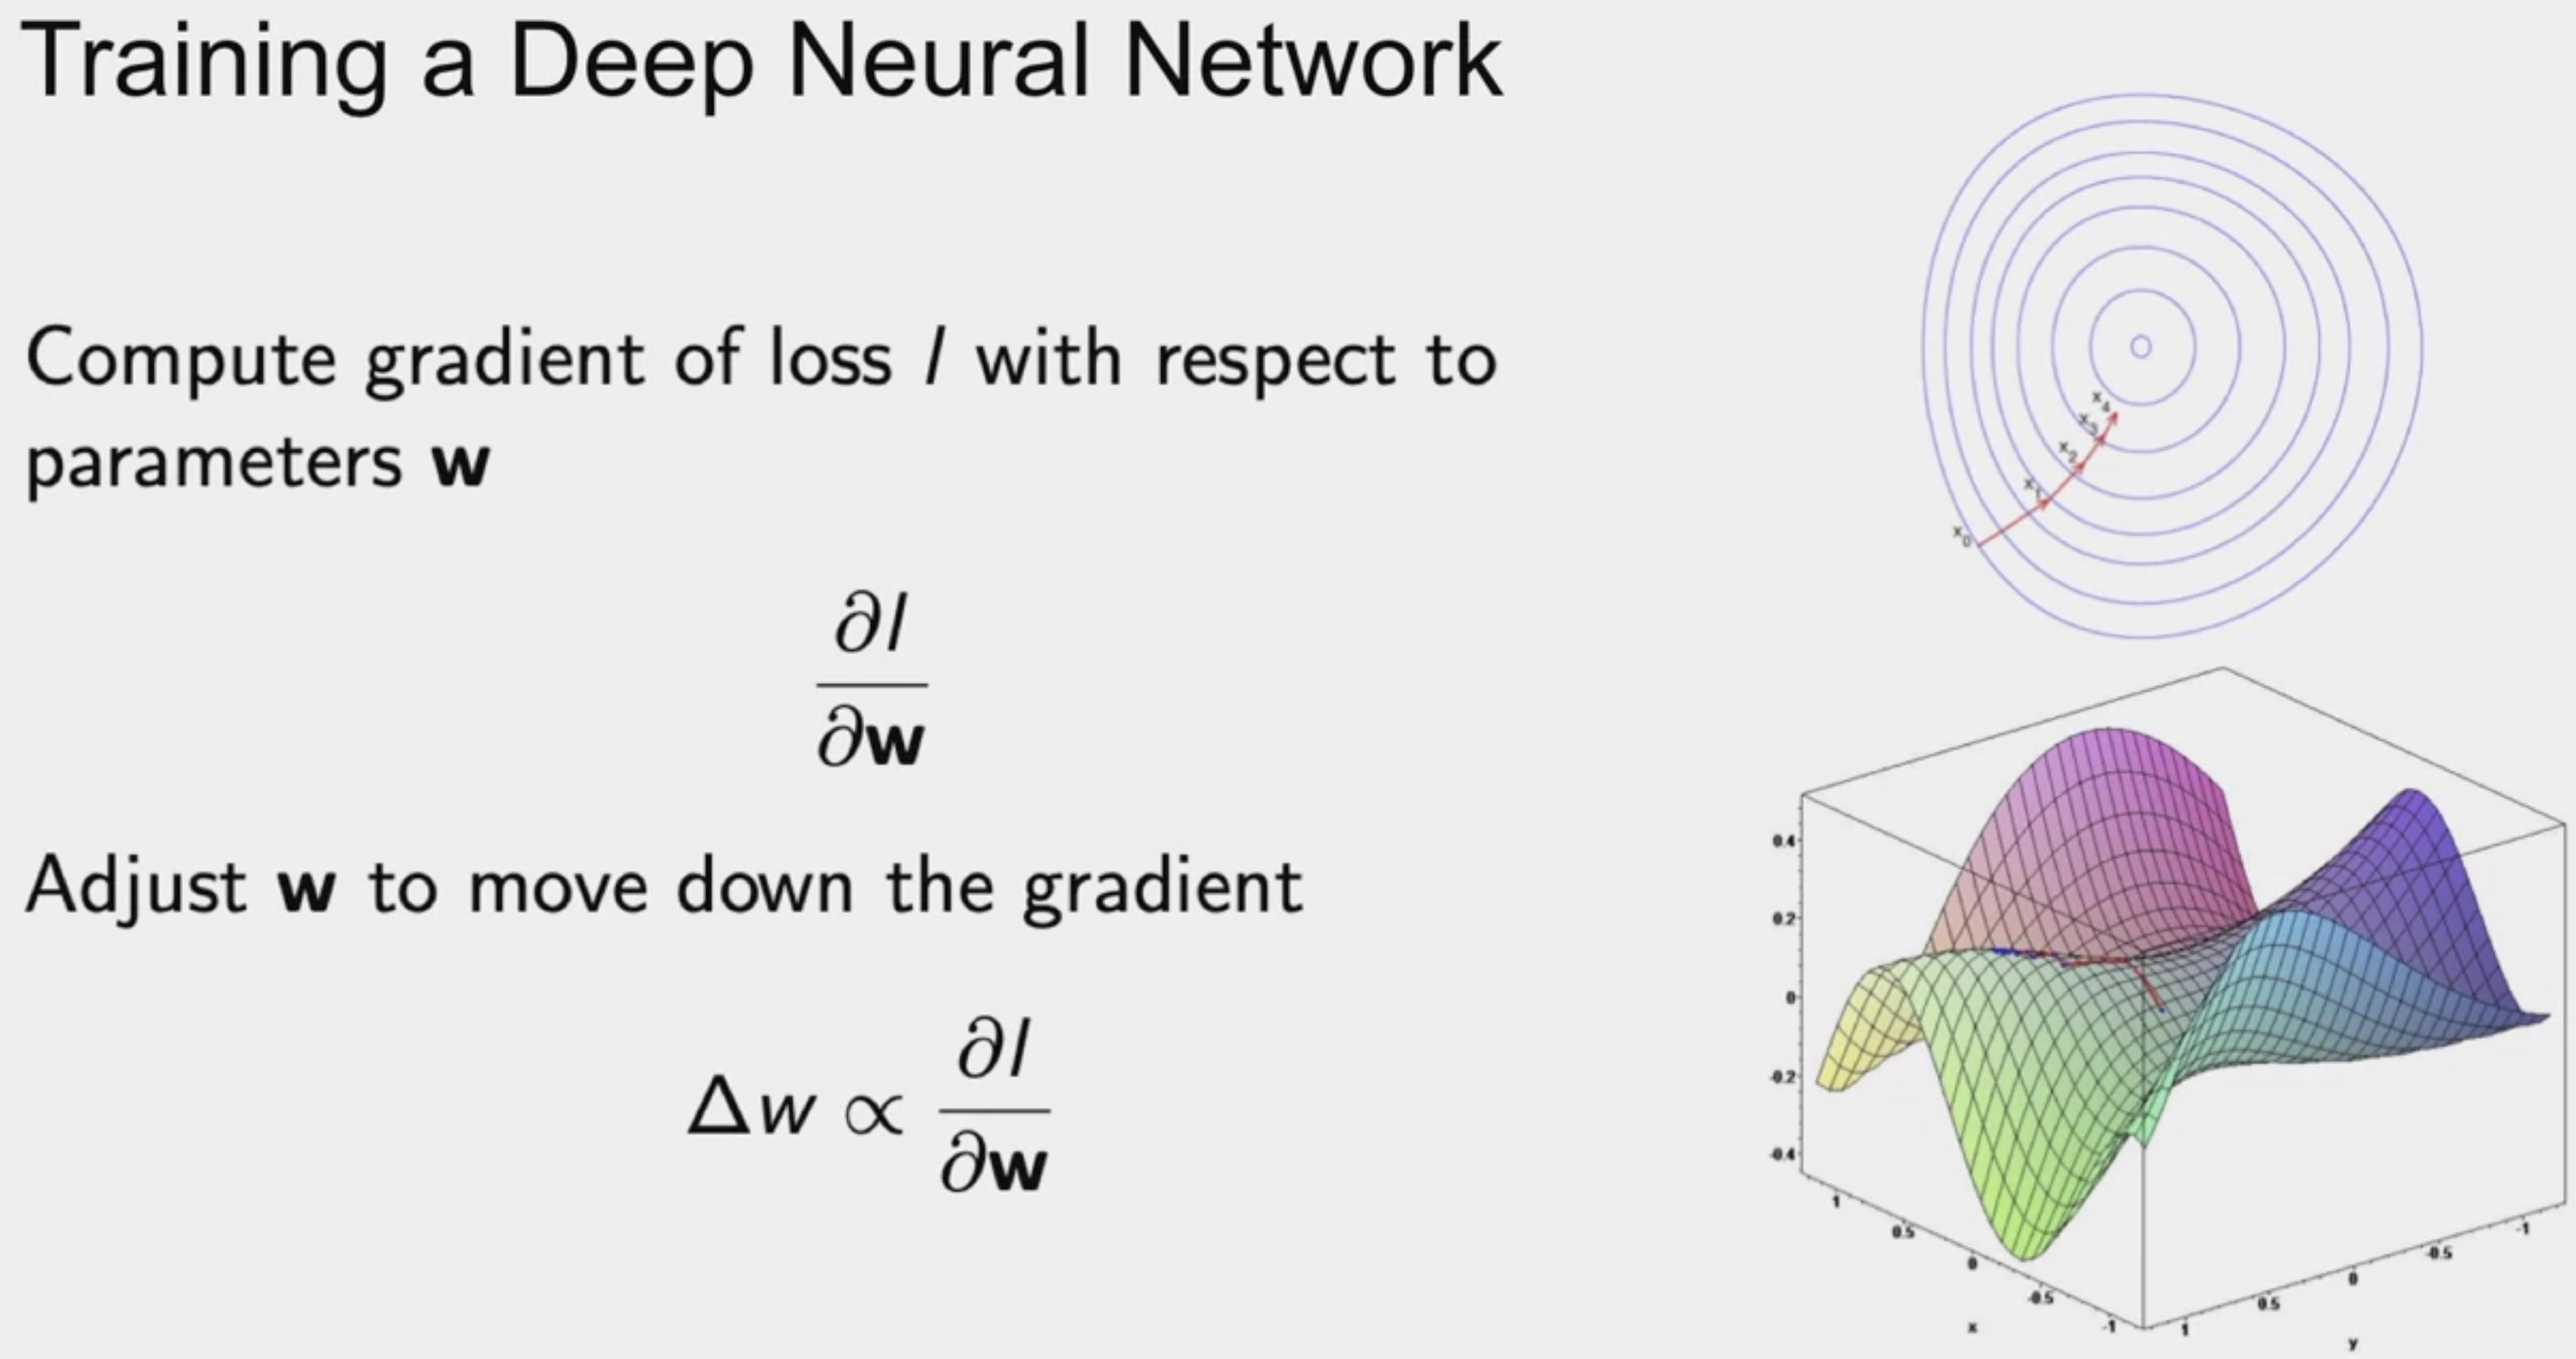
\includegraphics[width=0.9\columnwidth]{images/training-nn.png}
      \label{fig:training-nn}
  \end{figure}

  \item \textbf{Notation:}
  \begin{figure}[H]
    \centering
      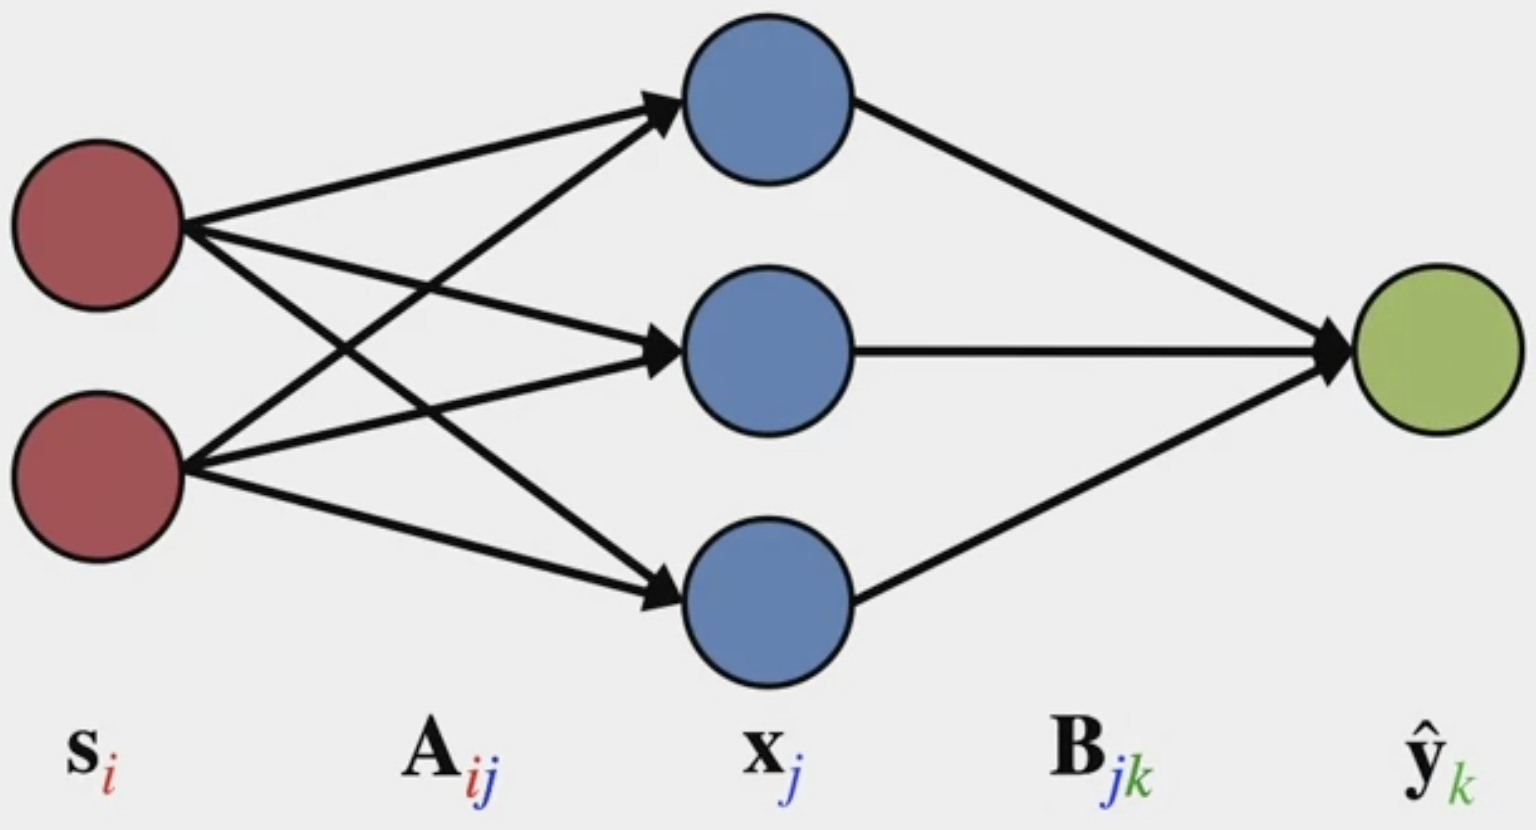
\includegraphics[width=0.5\columnwidth]{images/ann-notation.png}
      \label{fig:ann-notation}
  \end{figure}
  \begin{itemize}
    \item \textbf{weights (matrix) $A$} linearly weight $s$ to produce the features $x$
    \item \textbf{weights (matrix) $B$} linearly weight $x$ to produce the output $\hat{y}$
    \item \textbf{(output of hidden layer) $x$}$ \doteq f_A(\psi)$
    \begin{itemize}
      \item $\psi \doteq sA$
    \end{itemize}
    \item \textbf{(final output) $\hat{y}$} $\doteq f_B(\theta)$
    \begin{itemize}
      \item $\theta \doteq xB$
    \end{itemize}
  \end{itemize}


  \item The errors $\delta B$ from the output of the network are propagated backwards to this earlier layer to help determine the role $A$ had in producing that error ($\delta A$).


  \item \textbf{Full derivation (deriving the gradient):}
  \begin{itemize}


    \item \textbf{Gradient for $B$:}
    \begin{enumerate}
      \item Take the \textcolor{Purple}{partial derivative} \uline{\textbf{of} the \textbf{loss function $L(\hat{y}_k, y_k)$}} \uline{\textbf{with respect to} the first set of \textbf{weights $B$}}: $\frac{\partial L(\hat{y}_k, y_k)}{\partial B_{jk}}$
      \begin{itemize}
        \item We use the \textcolor{Purple}{chain rule} given the \uline{derivative of $L$ with respect to $\hat{y}$} \textbf{times} the \uline{derivative of $\hat{y}$ with respect to $B$}:
        $$
        \frac{\partial L(\hat{y}_k, y_k)}{\partial B_{jk}} = \frac{\partial L(\hat{y}_k, y_k)}{\partial \hat{y}_k} \cdot \textcolor{Blue}{\frac{\partial \hat{y}_k}{\partial B_{jk}}}
        $$
      \end{itemize}
      \item Use the \textcolor{Purple}{chain rule} again for this: \textcolor{Blue}{$\frac{\partial \hat{y}_k}{\partial B_{jk}}$} derivative:
      $$
      \frac{\partial L(\hat{y}_k, y_k)}{\partial B_{jk}} = \frac{\partial L(\hat{y}_k, y_k)}{\partial \hat{y}_k} \cdot \textcolor{Blue}{\frac{\partial f_B(\theta_k)}{\partial \theta_k} \cdot \frac{\partial \theta_k}{\partial B_{jk}}}
      $$
      \begin{itemize}
        \item Because $\theta$ is a linear function of $B$, and because $x$ does not depend on $B$:
        $$
        \frac{\partial \theta_k}{\partial B_{jk}} = x_j
        $$
        \item So general equation for $B$:
        $$
        \frac{\partial L(\hat{y}_k, y_k)}{\partial B_{jk}} = \frac{\partial L(\hat{y}_k, y_k)}{\partial \hat{y}_k} \cdot \textcolor{Blue}{\frac{\partial f_B(\theta_k)}{\partial \theta_k} \cdot x_j}
        $$
        \item To ease notation while computing the gradient with respect to $A$, let's define a new term $\delta^B$:
        $$
        \delta_k^B \doteq \frac{\partial L(\hat{y}_k, y_k)}{\partial \hat{y}_k} \cdot \frac{\partial f_B(\theta_k)}{\partial \theta_k}
        $$
      \end{itemize}
    \end{enumerate}
  \end{itemize}


  \item \textbf{Gradient for $A$:} The main difference is that we have one extra chain rule step because the weights $A$ also affect $x$.
  \begin{enumerate}
    \item Take the \textcolor{Purple}{partial derivative} \uline{\textbf{of} the \textbf{loss function $L(\hat{y}_k, y_k)$}} \uline{\textbf{with respect to} the second set of \textbf{weights $A$}}, combined with the previous chain rule step $\delta_k^B$: $\frac{\partial L(\hat{y}_k, y_k)}{\partial A_{ij}}$
    \begin{itemize}
      \item We use the \textcolor{Purple}{chain rule}:
      $$
      \frac{\partial L(\hat{y}_k, y_k)}{\partial A_{ij}} = \delta_k^B \cdot \textcolor{Blue}{\frac{\partial \theta_k}{\partial A_{ij}}}
      $$
    \end{itemize}
    \item Use the \textcolor{Purple}{chain rule} again for this: \textcolor{Blue}{$\frac{\partial \theta_k}{\partial A_{ij}}$} derivative:
    $$
    \frac{\partial L(\hat{y}_k, y_k)}{\partial A_{ij}} = \delta_k^B \cdot \textcolor{Blue}{B_{jk} \cdot \frac{\partial x_j}{\partial A_{ij}}}
    $$
    \item Using the \textcolor{Purple}{chain rule} again for \textcolor{Blue}{$\frac{\partial x_j}{\partial A_{ij}}$}, we get the derivative of \uline{$f_A(\psi)$ with respect to $\psi$} \textbf{times} the \uline{derivative of $\psi$ with respect to $A$}.
    $$
    \frac{\partial L(\hat{y}_k, y_k)}{\partial A_{ij}} = \delta_k^B \cdot B_{jk} \cdot \textcolor{Blue}{\frac{\partial f_A(\psi_j)}{\partial \psi_j} \cdot \frac{\partial \psi_j}{\partial A_{ij}}}
    $$
    \begin{itemize}
      \item Because $\psi = sA$, we get:
      $$
      \frac{\partial \psi_j}{\partial A_{ij}} = s_i
      $$
      \item So general equation for $A$:
      $$
      \frac{\partial L(\hat{y}_k, y_k)}{\partial A_{ij}} = \delta_k^B \cdot B_{jk} \cdot \textcolor{Blue}{\frac{\partial f_A(\psi_j)}{\partial \psi_j} \cdot s_i}
      $$
      \item We can clean up this derivative by again, defining a term $\delta^A$.
      $$
      \delta_j^A = (B_{jk} \delta_k^B) \frac{\partial f_A(\psi_j)}{\partial \psi_j}
      $$
    \end{itemize}
  \end{enumerate}

  \item \textbf{Both gradients $A$ and $B$ can now be rewritten in a similar form:}
  $$
  \frac{\partial L(\hat{y}_k, y_k)}{\partial A_{ij}} = \delta_j^A s_i
  $$
  $$
  \frac{\partial L(\hat{y}_k, y_k)}{\partial B_{jk}} = \delta_k^B x_j
  $$
  \begin{itemize}
    \item They have a term $\delta$ that contains an \uline{error signal times their input}.
  \end{itemize}
\end{itemize}





\begin{tcolorbox}[title={Backpropagation Algorithm (w. SGD)}]

\textbf{Gor each datapoint $(s,y)$ in dataset $D$:}
\begin{description}
    \item $\;\;\;$ Compute delta for $B$: $\delta_k^B \doteq \frac{\partial L(\hat{y}_k, y_k)}{\partial \hat{y}_k} \cdot \frac{\partial f_B(\theta_k)}{\partial \theta_k}$
    \item $\;\;\;$ Compute gradient for $B$: $\nabla_B^{jk} = \delta_k^B x_j$
    \item $\;\;\;$ $B \leftarrow B - \alpha_B \nabla_B$
\end{description}
\tcblower
\begin{description}
    \item $\;\;\;$ Compute delta for $A$: $\delta_j^A = (B_{jk} \delta_k^B) \frac{\partial f_A(\psi_j)}{\partial \psi_j}$
    \item $\;\;\;$ Compute gradient for $A$: $\nabla_A^{ij} = \delta_j^A s_i$
    \item $\;\;\;$ $A \leftarrow A - \alpha_A \nabla_A$
\end{description}
\end{tcolorbox}

Here we compute $\delta^A$ using $\delta^B$. Notice, that by computing the gradients of the end of the network first, we avoid recomputing the same terms for $A$, that were already computed for $\delta^B$. In fact, this is the main idea behind back propagation. It is simply gradient descent with this efficient strategy to compute gradients.

This derivation and algorithm easily extend to deeper networks. The $\delta$ for the earlier layer is similarly computed recursively using the $\delta$ in the next layer.

\bigskip

\textbf{Optimization Strategies for NNs}
\begin{itemize}
  \item \textbf{Weight Initialization:}
  \begin{itemize}
    \item \textbf{Motivation:} Choice of $w$ starting points can play a big role in the performance of the neural network.
    \item \textbf{Common Strategies:}
    \begin{itemize}
      \item \textbf{Random Sample}: One simple yet effective initialization strategy, is to randomly sample the initial weights from a normal distribution with small variance.
      $$
      w_{init} \sim \mathcal{N}(0,1)
      $$
      \begin{itemize}
        \item This way, each neuron has a different output from other neurons within its layer. This provides a more diverse set of potential features. By keeping the variants small, we ensure that the output of each neuron is within the same range as its neighbors.
        \item One downside to this strategy is that, \textcolor{red}{as we add more inputs to a neuron, the variance of the output grows}.
      \end{itemize}
      \item \textbf{Scaled Random Sample}: gets around the variance issue of 'Random Sample' by scaling the variance of the weights, by one over the square root of the number of inputs.
      $$
      w_{init} \sim \frac{\mathcal{N}(0,1)}{\sqrt{n_{inputs}}}
      $$
    \end{itemize}
  \end{itemize}
  \item \textbf{More sophisticated update mechanisms:}
  \begin{itemize}
    \item \textbf{Motivation:} More sophisticated update mechanisms can speed up neural network optimization.
    \item \textbf{Common Strategies:}
    \begin{itemize}
      \item \textbf{Momentum (heavy-ball method)}: similar to the regular stochastic gradient descent update plus an extra term called the momentum $M$.
      \begin{gather}
        w_{t+1} \leftarrow w_t - a \nabla_w L(w_t) + \textcolor{blue}{\lambda M_t} \\
        \textcolor{blue}{M_{t+1}} \leftarrow \textcolor{blue}{\lambda M_t} - \alpha \nabla_w L
      \end{gather}
      \begin{itemize}
        \item The momentum term summarizes the history of the gradients using a decaying sum of gradients with decay rate Lambda.
          \item[] $\;\;\; *$ If recent gradients have all been in similar directions, then we gained momentum in that direction. This means, we make a large step in that direction.
          \item[] $\;\;\; *$ If recent updates have conflicting directions, then it kills the momentum. The momentum term will have little impact on the update and we will make a regular gradient descent step.
      \end{itemize}
      \item \textbf{Vector step-size adaption}: uses a separate step size for each weight in the network.
      \begin{itemize}
        \item Global scalar step size is problematic because it can result in updates that are too big for some weights and too small for other weights.
      \end{itemize}
    \end{itemize}
  \end{itemize}
\end{itemize}

























\section{On-policy Control with Approximation}\label{on-policy-control-with-approximation}

In this chapter we return to the control problem, now with parametric approximation of the action-value function $\hat{q}(s,a,w) \approx q_*(s,a)$, where $w \in \mathbb{R}^d$ is a finite-dimensional weight vector. So the feature representation has to represent actions as well.



With \textbf{discrete action spaces} we can \uline{make feature representation to represent actions as well} by have a separate function approximator for each action. This can be accomplished by stacking the features.

\begin{figure}[H]
  \centering
    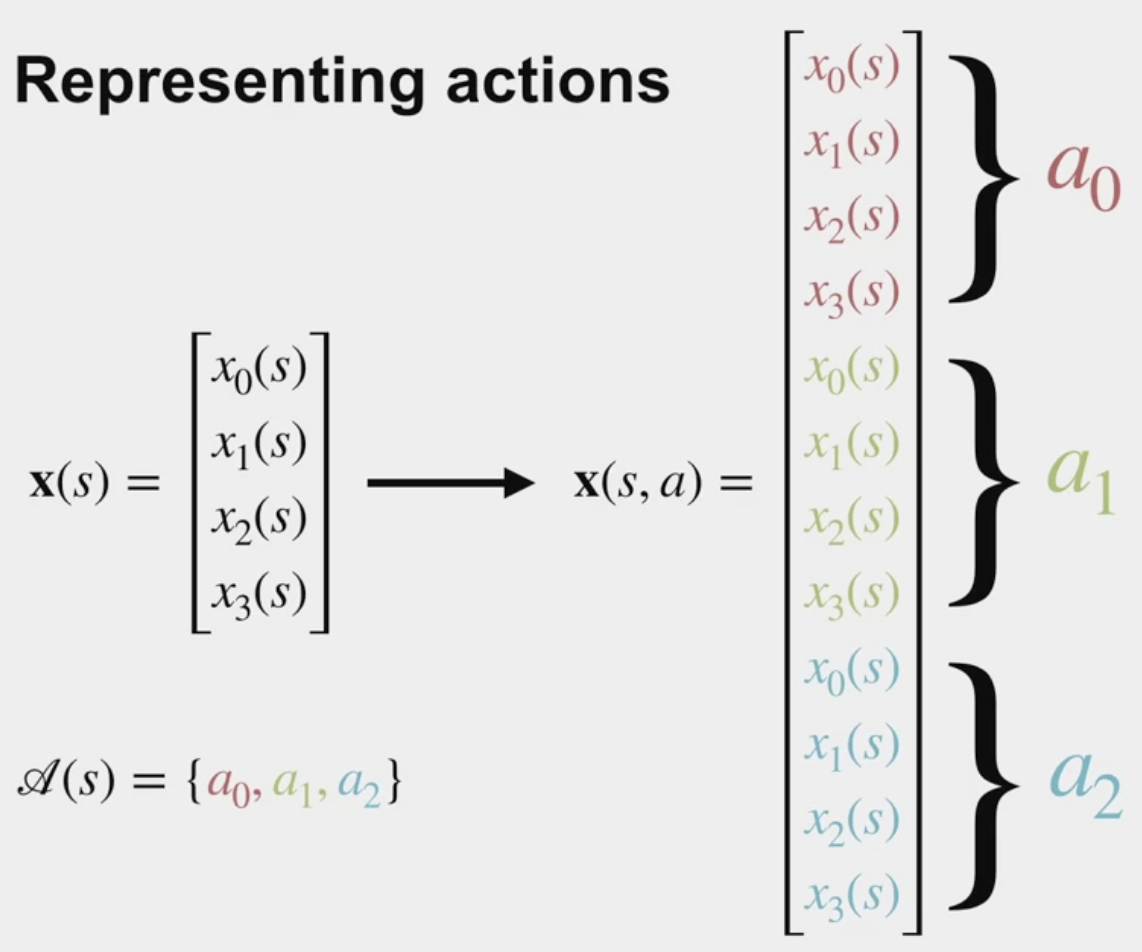
\includegraphics[width=0.8\columnwidth]{images/stacked-feature-representation-eg.png}
    \caption{Example stacked feature representation for 4 features (representing states), and 3 actions.}
    \label{fig:stacked-feature-representation-eg}
\end{figure}

The action values are then the dot products between each segment of the weight vector and the feature vector.

\begin{figure}[H]
  \centering
    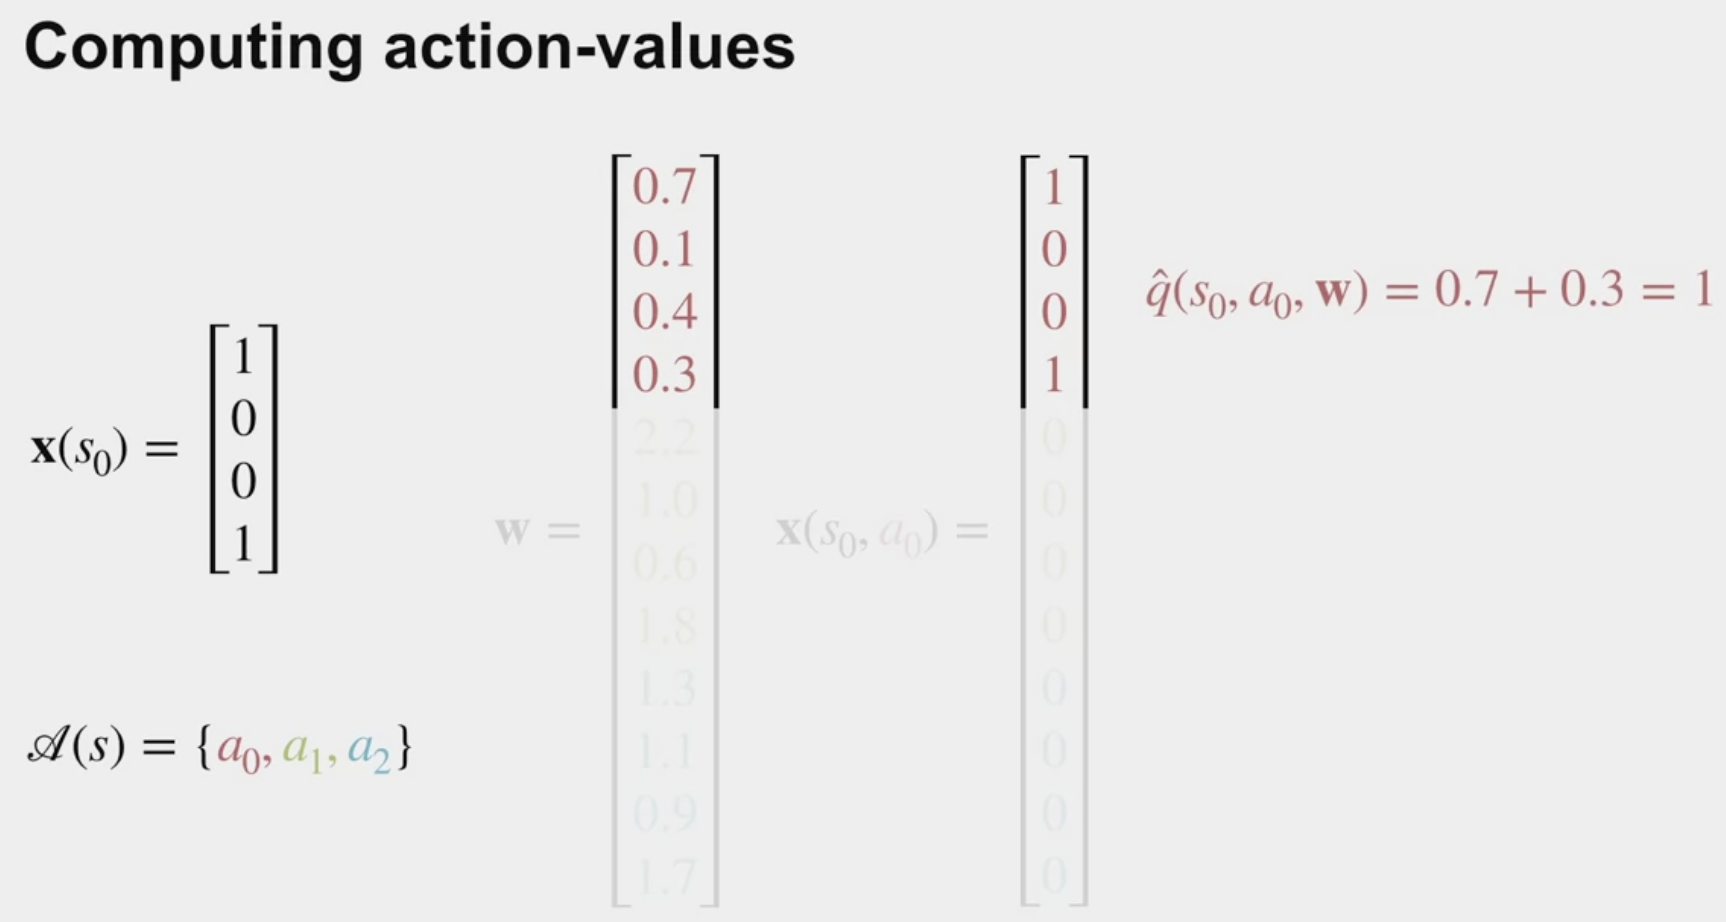
\includegraphics[width=0.9\columnwidth]{images/stacked-feature-representation-eg2.png}
    \caption{Example of calculating action-value for $s_0$ and $a_0$.}
    \label{fig:stacked-feature-representation-eg2}
\end{figure}

For \textbf{continuous action spaces} or if you want to \textbf{generalize over actions}, the \uline{action can be passed as an input} like any other state variable.

For NNs we would input both the state and the action to the network. There would only be one output. The approximate action value for that state and action.

\begin{figure}[H]
  \centering
    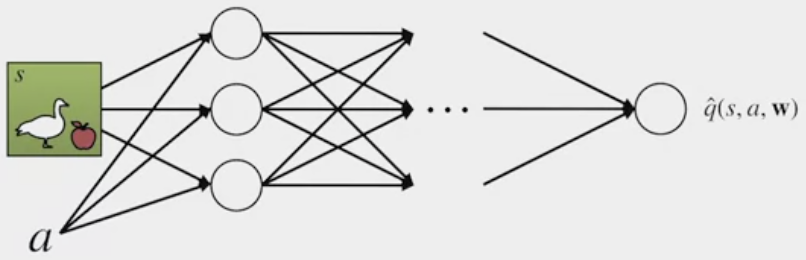
\includegraphics[width=0.6\columnwidth]{images/action-values-with-ann.png}
    \label{fig:action-values-with-ann}
\end{figure}









\subsection{Episodic Sarsa with Function Approximation}\label{episodic-sarsa-with-function-approximation}

\textbf{Difference to tabular SARSA:}
We \textbf{use} \uline{parameterized action value functions $\hat{q}(s,a,w)$} \textbf{for} the \uline{action-value estimates}. The update also changes to use the gradient to update the weights similar to semi-gradient TD.


\begin{tcolorbox}[title={Episodic Semi-gradient Sarsa for Estimating $\hat{q} \approx q_*$}]

\textbf{Input:} a differentiable action-value function parameterization $ \;\;\;\;\;\;\;\;\;\;\;\;\;\;\;\; \hat{q}: \mathcal{S} \times \mathcal{A} \times \mathbb{R}^d \rightarrow \mathbb{R}$

\textbf{Algorithm parameters:} $\alpha > 0$ \& small $\epsilon > 0$

\textbf{Initialize:} value-function weights $w \in \mathbb{R}^d$ arbitrarily (e.g., $w=0$) \\

\textbf{Loop for each episode:}
\begin{description}
   \item $\;\;\;$ $S, A \leftarrow$ initial state and action of episode (e.g., $\epsilon$-greedy)
   \item $\;\;\;$ \textbf{Loop for each step of episode:}
   \begin{description}
     \item $\;\;\;$ Take action $A$ observe $R, S'$
     \item $\;\;\;$ If $S'$ is terminal:
     \begin{description}
       \item $\;\;\;$ $w \leftarrow w + \alpha (R - \hat{q}(S,A,w))\nabla \hat{q}(S,A,w)$
       \item $\;\;\;$ Go to next episode
     \end{description}
     \item $\;\;\;$ Choose $A'$ as a function of $\hat{q}(S',\cdot,w)$ (e.g. $\epsilon$-greedy)
     \item $\;\;\;$ $w \leftarrow w + \alpha (R + \gamma \hat{q}(S',A',w) - \hat{q}(S,A,w))\nabla \hat{q}(S,A,w)$
     \item $\;\;\;$ $S \leftarrow S'; A \leftarrow A'$
   \end{description}
\end{description}
\end{tcolorbox}







\subsection{Expected Sarsa with Function Approximation}\label{episodic-sarsa-with-function-approximation}


\textbf{Sarsa into expected Sarsa:}

\begin{itemize}
  \item Recall Sarsa with function approximation:
  $$
  w \leftarrow w + \alpha (R_{t+1} + \gamma \hat{q}(S_{t+1},A_{t+1},w)- \hat{q}(S_t,A_t,w)) \nabla \hat{q}(S_t,A_t,w)
  $$
  \item Expected Sarsa with function approximation:
  $$
  w \leftarrow w + \alpha (R_{t+1} + \gamma \textcolor{blue}{\sum_{a'} \pi(a' | S_{t+1}) \hat{q}(S_{t+1}, a',w)} - \hat{q}(S_t,A_t,w)) \nabla \hat{q}(S_t,A_t,w)
  $$
  \begin{itemize}
    \item We compute the action values from our weight vector for every action in the next state. Then we compute this expectation under the target policy.
  \end{itemize}
\end{itemize}









\subsection{Exploration under Function Approximation}\label{exploration-under-function-approximation}

\textbf{Optimistic initial values} $\rightarrow$ initializing the weights such that the resulting values are optimistic (largest possible return).
\begin{itemize}
  \item Can be \textcolor{red}{difficult in complicated functions} like neural networks.
  \item Depending on how our features generalize, optimistic initial values \textcolor{red}{may not result in the same kind of systematic exploration we see in the tabular case}.
\end{itemize}

\textbf{$\epsilon$-greedy} is generally applicable and easy to use even in cases with non-linear function approximation.The only thing Epsilon greedy needs are the action value estimates, independent of how they are initialized or approximated.
\begin{itemize}
  \item However, Epsilon greedy is not a directed exploration method. It \uline{relies on randomness} to discover better actions near states followed by the current policy. It is therefore \textcolor{red}{not as systematic as exploration methods that rely on optimism}.
\end{itemize}








\subsection{Average Reward: A New Problem Setting for Continuing Tasks}\label{awerage-reward-problem-setting-for-continuing-tasks}


\textbf{What:} Average Reward Formulation, a new way of formulating continuing problems.

\textbf{Why:} In continuing tasks, we might be interested in \uline{extremely long horizon performance}.

\textbf{How:} it cares equally about nearby and distant rewards.


\begin{itemize}
  \item \textbf{Average Reward Objective:}
  $$
  r(\pi) \doteq \lim_{h\to\infty} \frac{1}{h} \sum_{t=1}^h \mathbb{E}[R_t | S_0, A_{0:t-1} \sim \pi]
  $$
  \item More generally using the state visitation, $\mu$:
  $$
  r(\pi) = \sum_s \mu_\pi(s) \sum_a \pi(a | s) \sum_{s',r} p(s',r|s,a)r
  $$
  \begin{itemize}
    \item This inner term is the expected reward in a state under policy $\pi$. The outer sum takes the expectation over how frequently the policy is in that state. Together, we get the expected reward across states (average reward for a policy).
  \end{itemize}
\end{itemize}



Deciding which actions from a state are better? What we need are action values for this new setting?
\begin{itemize}
  \item \textbf{\textcolor{blue}{Differential Returns}:} In the average reward setting, returns are \textbf{defined} in terms of \uline{differences between \textcolor{blue}{rewards $R$} and the \textcolor{blue}{average reward $r(\pi)$}}.
  \begin{gather*}
  G_t = R_{t+1} - r(\pi) + R_{t+2} - r(\pi) + R_{t+3} - r(\pi) + ...
  \end{gather*}
  \item \textbf{represents} how much more reward the agent will receive from the current state and action compared to the average reward of the policy.
  \item The differential return can only be used to compare actions if the same policy is followed on subsequent time steps. To compare policies, their average reward should be used instead.
  \item Here $q_\pi(s,a) = \mathbb{E}_\pi[G_t | S_t = s, A_t = a]$ captures \uline{how much more reward the agent will get by starting in a particular state} than it would get on average over all states if it followed a fixed policy.
  $$
  q_\pi(s,a) = \sum_{s',r} p(s',r | s,a) (r-r(\pi) + \sum_{a'} \pi(a'|s') q_\pi(s',a'))
  $$
\end{itemize}
































\section{*Off-policy Methods with Approximation}\label{off-policy-methods-with-approximation}

The extension to function approximation turns out to be significantly different and harder for off-policy learning than it is for on-policy learning.

In this chapter we explore the convergence problems, take a closer look at the theory of linear function approximation, introduce a notion of learnability, and then discuss new algorithms with stronger convergence guarantees for the off-policy case. In the end we will have improved methods, but the \textcolor{red}{theoretical results will not be as strong, nor the empirical results as satisfying, as they are for on-policy learning}.




\subsection{Q-learning with Function Approximation}\label{qlearning-with-function-approximation}



Q-learning is a special case of expected Sarsa


\begin{itemize}
  \item Recall, Expected Sarsa with function approximation:
  $$
  w \leftarrow w + \alpha (R_{t+1} + \gamma \textcolor{blue}{\sum_{a'} \pi(a' | S_{t+1}) \hat{q}(S_{t+1}, a',w)} - \hat{q}(S_t,A_t,w)) \nabla \hat{q}(S_t,A_t,w)
  $$
  \item Q-learning with function approximation:
  $$
  w \leftarrow w + \alpha (R_{t+1} + \gamma \textcolor{blue}{\max_{a'} \hat{q}(S_{t+1}, a',w)} - \hat{q}(S_t,A_t,w)) \nabla \hat{q}(S_t,A_t,w)
  $$
  \begin{itemize}
    \item In Q-learning, the target policy is greedy with respect to the approximate action values. Computing the expectation under greedy policy is the same as computing the maximum action value.
  \end{itemize}
\end{itemize}








\end{document}
